%%%%%%%%%%%%%%%%%%%%%%%%%%%%%%%%%%%%%%%%%
% Beamer Presentation
% LaTeX Template
% Version 1.0 (10/11/12)
%
% This template has been downloaded from:
% http://www.LaTeXTemplates.com
%
% License:
% CC BY-NC-SA 3.0 (http://creativecommons.org/licenses/by-nc-sa/3.0/)
%
%%%%%%%%%%%%%%%%%%%%%%%%%%%%%%%%%%%%%%%%%

%----------------------------------------------------------------------------------------
%	PACKAGES AND THEMES
%----------------------------------------------------------------------------------------

\documentclass{beamer}

\mode<presentation> {

% The Beamer class comes with a number of default slide themes
% which change the colors and layouts of slides. Below this is a list
% of all the themes, uncomment each in turn to see what they look like.

%\usetheme{default}
%\usetheme{AnnArbor}
%\usetheme{Antibes}
%\usetheme{Bergen}
%\usetheme{Berkeley}
%\usetheme{Berlin}
%\usetheme{Boadilla}
%\usetheme{CambridgeUS}
%\usetheme{Copenhagen}
%\usetheme{Darmstadt}
%\usetheme{Dresden}
%\usetheme{Frankfurt}
%\usetheme{Goettingen}
%\usetheme{Hannover}
%\usetheme{Ilmenau}
%\usetheme{JuanLesPins}
%\usetheme{Luebeck}
%\usetheme{Madrid}
%\usetheme{Malmoe}
%\usetheme{Marburg}
%\usetheme{Montpellier}
%\usetheme{PaloAlto}
%\usetheme{Pittsburgh}
%\usetheme{Rochester}
%\usetheme{Singapore}
\usetheme{Szeged}
%\usetheme{Warsaw}

% As well as themes, the Beamer class has a number of color themes
% for any slide theme. Uncomment each of these in turn to see how it
% changes the colors of your current slide theme.

%\usecolortheme{albatross}
\usecolortheme{beaver}
%\usecolortheme{beetle}
%\usecolortheme{crane}
%\usecolortheme{dolphin}
%\usecolortheme{dove}
%\usecolortheme{fly}
%\usecolortheme{lily}
%\usecolortheme{orchid}
%\usecolortheme{rose}
%\usecolortheme{seagull}
%\usecolortheme{seahorse}
%\usecolortheme{whale}
%\usecolortheme{wolverine}

%\setbeamertemplate{footline} % To remove the footer line in all slides uncomment this line
%\setbeamertemplate{footline}[page number] % To replace the footer line in all slides with a simple slide count uncomment this line

%\setbeamertemplate{navigation symbols}{} % To remove the navigation symbols from the bottom of all slides uncomment this line
}

\usepackage{graphicx} % Allows including images
\usepackage{booktabs} % Allows the use of \toprule, \midrule and \bottomrule in tables
\usepackage{hyperref}
\usepackage{xcolor}

%----------------------------------------------------------------------------------------
%	TITLE PAGE
%----------------------------------------------------------------------------------------

\title[L0 Upgrade]{Layer 0 Upgrade Detector} % The short title appears at the bottom of every slide, the full title is only on the title page

\author{Matt Solt} % Your name
\institute[Stanford] % Your institution as it will appear on the bottom of every slide, may be shorthand to save space
{
SLAC National Accelerator Laboratory \\ % Your institution for the title page
\medskip
\textit{mrsolt@slac.stanford.edu} % Your email address
}
\date{\today} % Date, can be changed to a custom date

\begin{document}

\begin{frame}
\titlepage % Print the title page as the first slide
\end{frame}

%----------------------------------------------------------------------------------------
%	PRESENTATION SLIDES
%----------------------------------------------------------------------------------------

%------------------------------------------------
%\section{First Section} % Sections can be created in order to organize your presentation into discrete blocks, all sections and subsections are automatically printed in the table of contents as an overview of the talk
%------------------------------------------------

%\subsection{Subsection Example} % A subsection can be created just before a set of slides with a common theme to further break down your presentation into chunks

\begin{frame}
\frametitle{Introduction}
\begin{itemize}
\item HPS is \textcolor{darkgray}{\textbf{planning on upgrading the existing SVT by adding another tracking layer}} between the target and current 1st layer
\item This should drastically \textcolor{darkgray}{\textbf{improve our vertexing reach}}
\item Tracking layers 2 and 3 are also being moved towards the beam for increased long-lived A' acceptance
\item \textcolor{darkgray}{\textbf{Reach comparison}} for the first layer hit requirements as well as other relevant simulations are presented
\item Increased backgrounds studies due to upgrade are also presented
\end{itemize}

\end{frame}

%------------------------------------------------

%\begin{frame}
%\frametitle{L0 Upgrade Description}
%\begin{itemize}
%\item L0 upgrade includes \textcolor{darkgray}{\textbf{adding 7th tracking layer}} between the target and current first layer
%\begin{itemize}
%\item \textcolor{darkgray}{\textbf{Improves vertex resolution}} (and hence vertexing reach), mass resolution, and n-hit tracking for the recoil electron
%\end{itemize}
%\end{itemize}
%\begin{figure}
%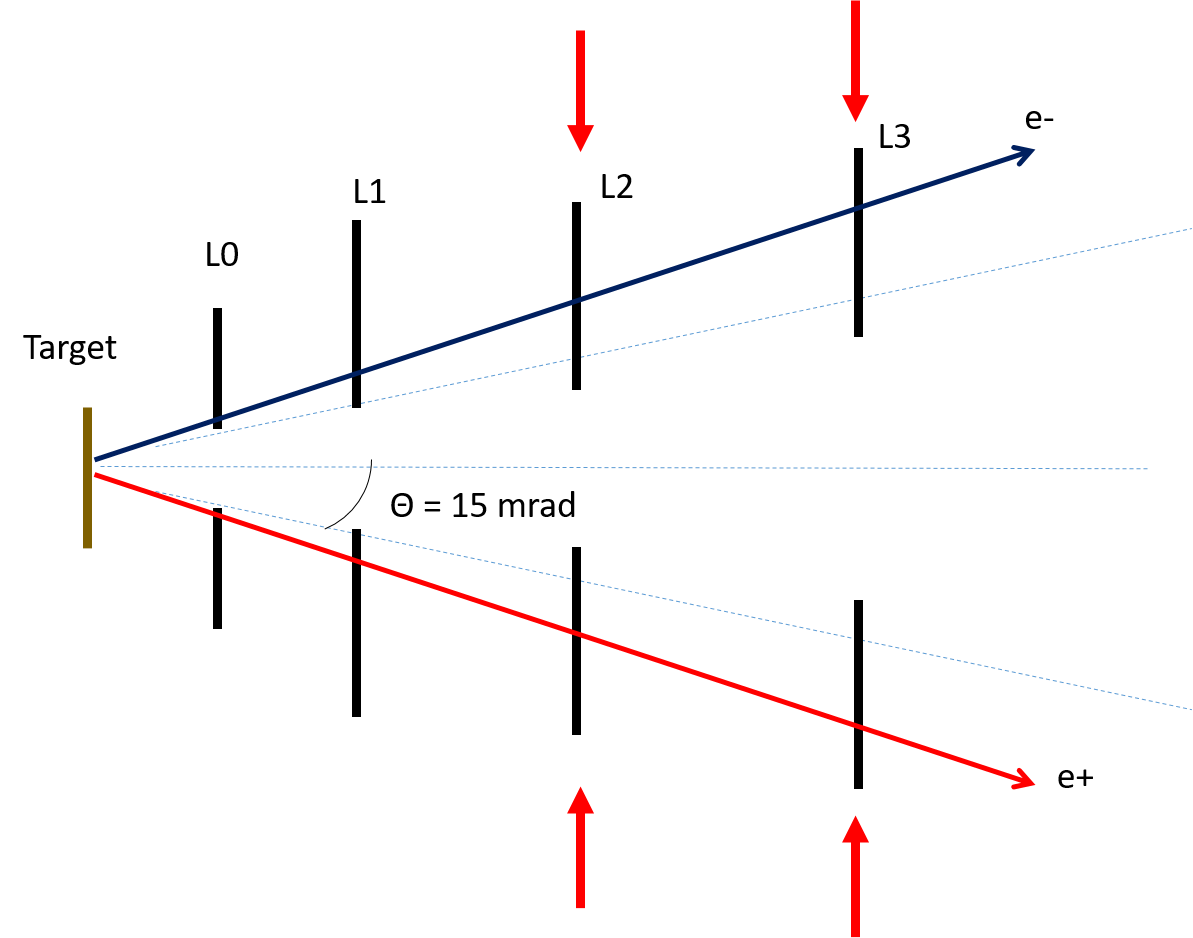
\includegraphics[width=0.6\linewidth]{figs/L0_schematic1.png}
%\end{figure}

%\end{frame}

%------------------------------------------------

%\begin{frame}
%\frametitle{L0 Upgrade Description (cont.)}
%\begin{itemize}
%\item L0 upgrade also includes moving tracking \textcolor{darkgray}{\textbf{layers 2 and 3 towards the beam by $0.8$ mm}}
%\begin{itemize}
%\item \textcolor{darkgray}{\textbf{Improves acceptance for long-lived A's}} (and hence the vertexing reach)
%\end{itemize}
%\end{itemize}
%\begin{figure}
%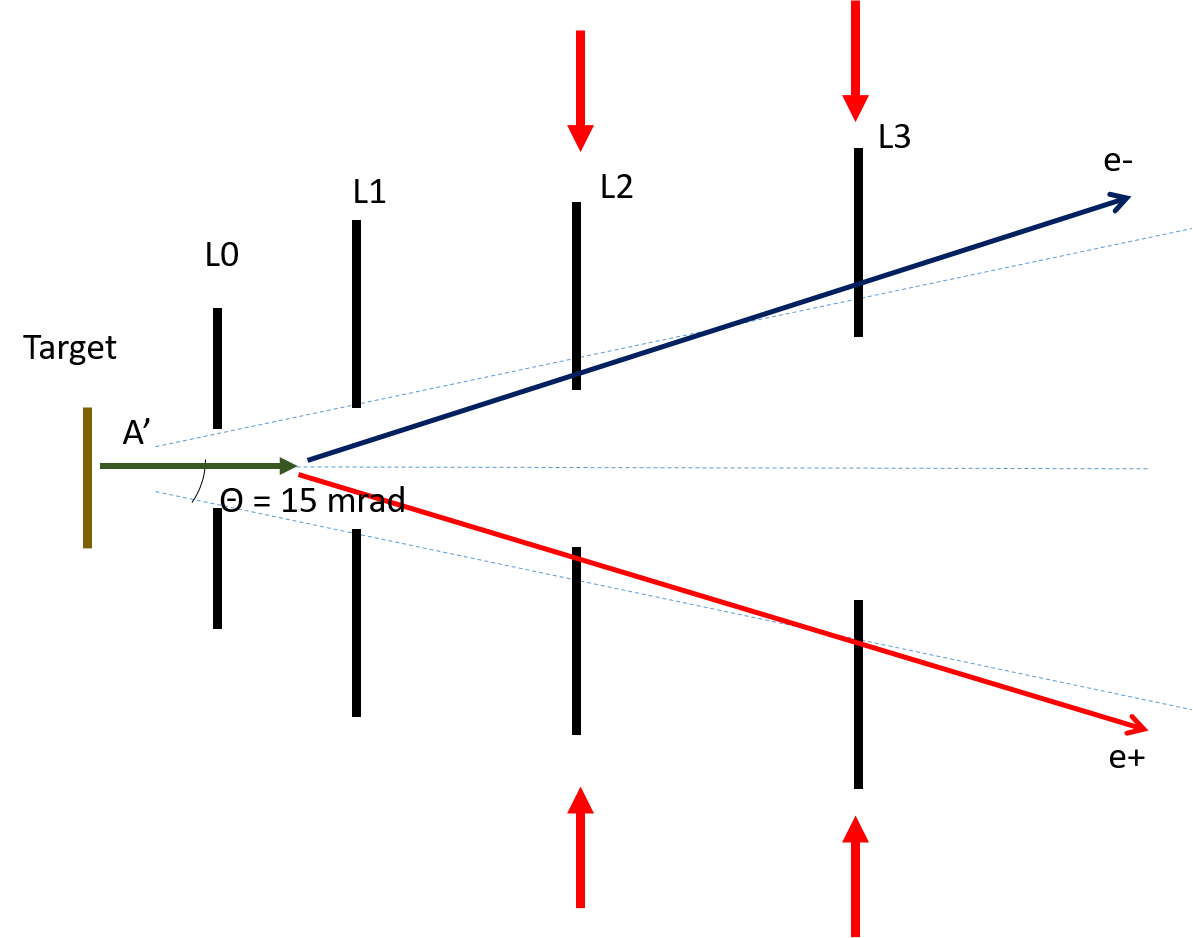
\includegraphics[width=0.6\linewidth]{figs/L0_schematic2.png}
%\end{figure}

%\end{frame}

%------------------------------------------------

\begin{frame}
\frametitle{L0 Upgrade Simulation Dimensions}
\begin{itemize}
\item Layer 0 sensor will contain 256 channels per sensor (no intermediate strip), an axial and stereo sensor on top/bottom and positron/electron side. Each sensor is 10 x 14.08 mm and strips are 200 microns in simulation (aiming for 150 microns)
\item Nominal has 640 readout channels (with intermediate strip), an axial stereo sensor on top/bottom and positron/electron side for layers 4-6. Each sensor is 100 x 38.4 mm and strips are 250 microns
\end{itemize}
\begin{figure}
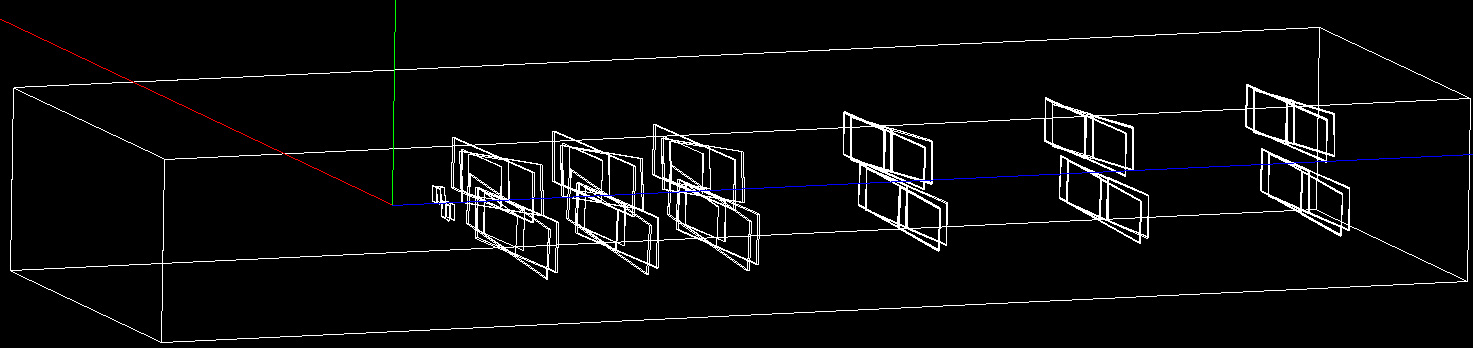
\includegraphics[width=0.8\linewidth]{figs/L0_schematic.PNG}
\end{figure}

\end{frame}

%------------------------------------------------

\begin{frame}
\frametitle{L0 Monte Carlo}
\begin{itemize}
\item A lot of computing time spent on L0 MC (thanks Brad), lots of troubleshooting, and still a few issues to be solved
\item \textcolor{darkgray}{\textbf{tritrig-wab-beam}} - wabs with beam background combined with tridents with beam background at enhanced rate
\begin{itemize}
\item Normalized by trident rate $155 \frac{1}{nb}$ (about 13\% of 2015 total luminosity at 0.5 mm) for both nominal and L0 (direct comparison)
\item wabs are NOT enhanced, so these are underestimated. Eventually will have the correct proportions
\item Skeptical of this normalization (probably about 75\% luminosity over-estimate) based on rates compared to tritrig + wab and wab-beam-tri and data
\item Goal is to obtain total 2015 luminosity at 0.5 mm
\item Used to fit vertex tails to compute zcut, rate is used for reach plots
\end{itemize}
\end{itemize}

\end{frame}

%------------------------------------------------

\begin{frame}
\frametitle{L0 Monte Carlo (cont.)}
\begin{itemize}
\item \textcolor{darkgray}{\textbf{Pure wabs, radiatives, and tridents (tritrig)}}
\begin{itemize}
\item Used to compute radiative fraction ($\frac{radiatives}{wabs + tridents}$)
\item MG5 radiatives for L0 are on the way
\end{itemize}
\item \textcolor{darkgray}{\textbf{wab-beam-tri}} - closest MC we have to beam
\begin{itemize}
\item 30 s of beam for L0; 10 s of beam for nominal
\item Used for backround studies - trigger rates, occupancies, wab conversion rates, and beam background rates
\end{itemize}
\item \textcolor{darkgray}{\textbf{Prompt and displaced A's}}
\begin{itemize}
\item Used for acceptance and efficiency studies and mass resolution
\end{itemize}
\end{itemize}

\end{frame}

%------------------------------------------------

\begin{frame}
\frametitle{L0 Studies}
\begin{itemize}
\item Acceptance (prompt A's)
\item Invariant Mass (Displaced A's)
\item Displaced Efficiency $\frac{A's \ Detectable \ after \ cuts}{A' \ truth}$ (Displaced A's)
\item Vertex Tail Fitting and Z Cuts
\item Reach Plots for First Layer Hit Requirements
\item Future Plans for Reach Plots Using Other Layer Requirements
\item Backgrounds
\begin{itemize}
\item Increased converted wabs due to L0 and moving L2/L3
\item Occupancies (in the near future)
\end{itemize}
\item Detailed plots here: \href{https://confluence.slac.stanford.edu/display/hpsg/Layer+0+Studies}{\textcolor{red}{\textbf{L0 Plots}}}
\end{itemize}

\end{frame}

%------------------------------------------------

\begin{frame}
\frametitle{Acceptance}
\begin{itemize}
\item \textcolor{darkgray}{\textbf{Geometrical acceptance}} for prompt A's as a function of mass for 1.05 GeV, 2.3 GeV, and 4.4 GeV beam energies
\item The comparison is 5 hits in the nominal detector compared to 6 hits in L0 detector
\end{itemize}
\begin{figure}
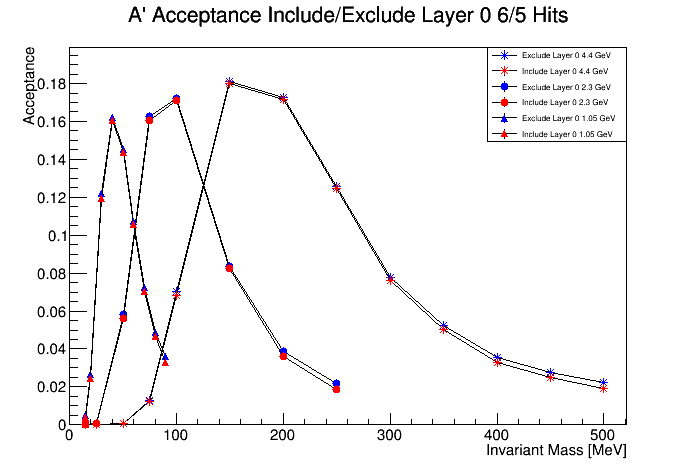
\includegraphics[width=0.6\linewidth]{figs/TridentAcceptanceInL0ExL05hit.png}
\end{figure}

\end{frame}

%------------------------------------------------

\begin{frame}
\frametitle{Cuts}
\begin{itemize}
\item Analysis divided into \textcolor{darkgray}{\textbf{mutually exclusive layer requirement}} categories
\begin{itemize}
\item Nominal total reach = L1L1 + L1L2 + L2L2
\item Upgrade total reach = L0L0 + L0L1 + L1L1 + L1L2 + L2L2 + L0L2
\end{itemize}
\item L0 Track $\chi^2<35$ and shared hits must be less than 4
\item Current \textcolor{darkgray}{\textbf{cuts eliminate about 20\% more A' and background in L0}}
\end{itemize}
\begin{figure}
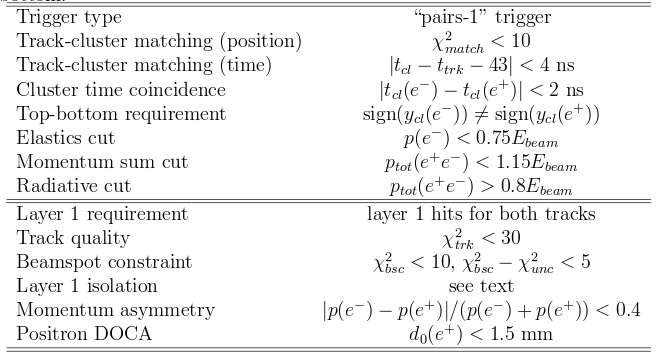
\includegraphics[width=0.6\linewidth]{figs/cuts.png}
\end{figure}

\end{frame}

%------------------------------------------------

\begin{frame}
\frametitle{Mass Vertex Resolution Improvement} %+ Radiative Fraction}
\begin{itemize}
\item \textcolor{darkgray}{\textbf{Displaced A' mass resolution}} for unconstrained V0s %(left) and radiative fraction (right)
\end{itemize}
\begin{figure}
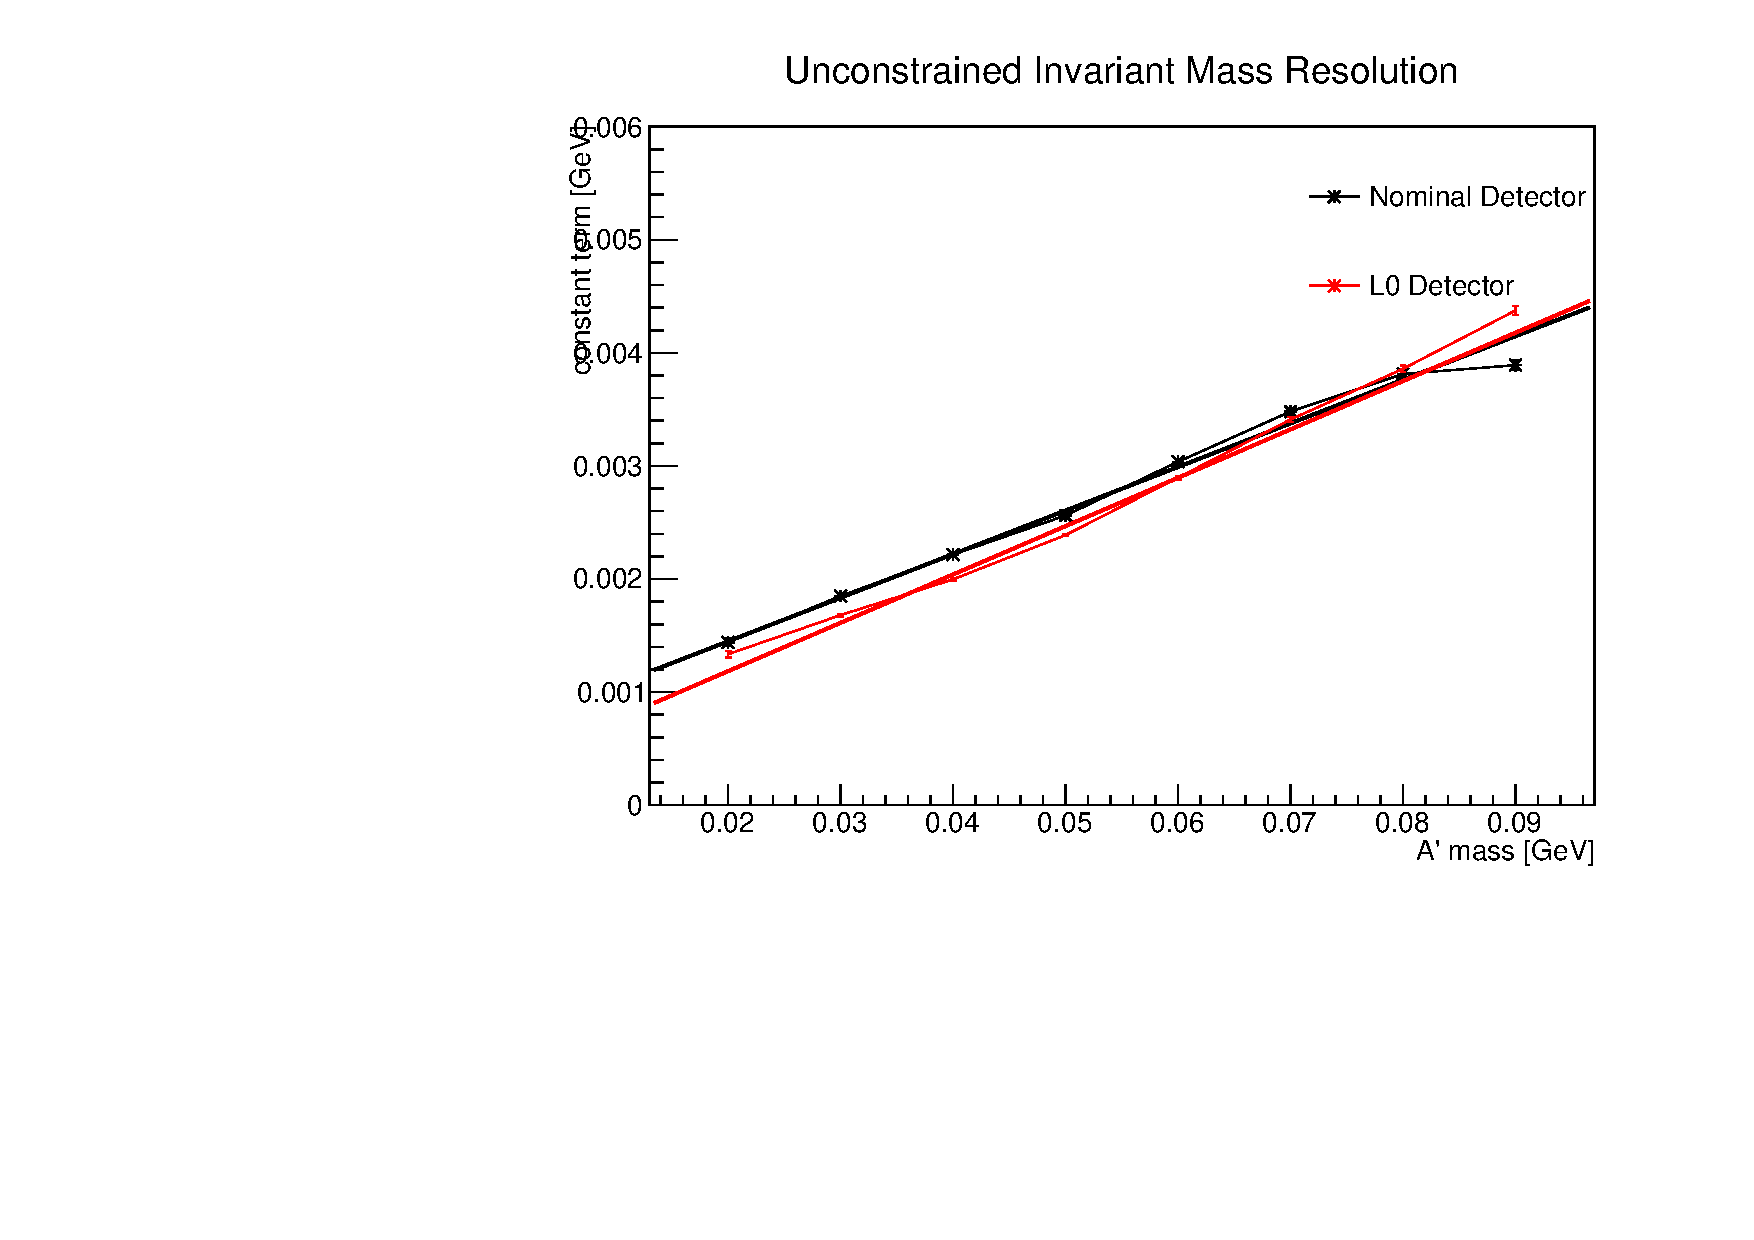
\includegraphics[width=0.55\linewidth]{figs/mass_res.pdf}
%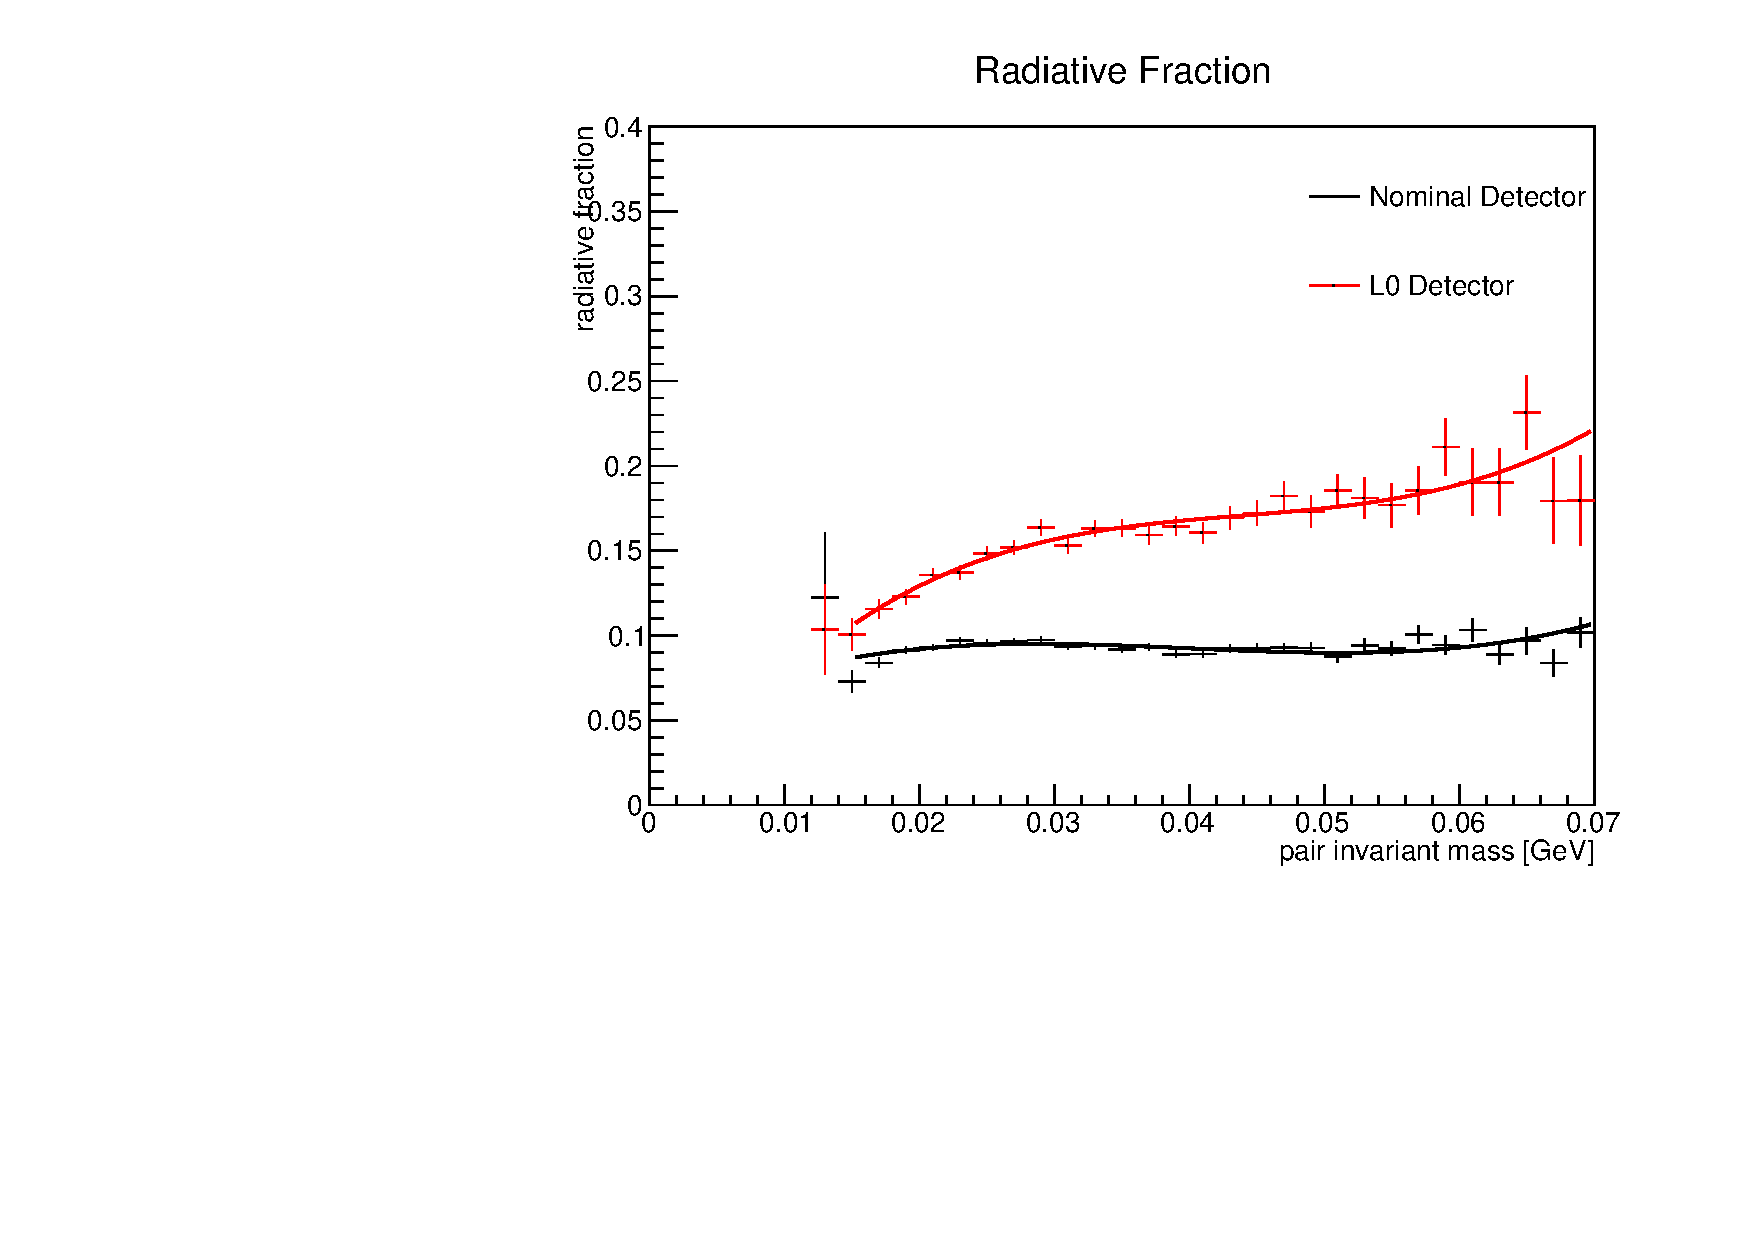
\includegraphics[width=0.55\linewidth]{figs/frac.pdf}
\end{figure}

\end{frame}

%------------------------------------------------

\begin{frame}
\frametitle{Long-lived A' Efficiency Improvement}
\begin{itemize}
\item Moving in L2 and L3 \textcolor{darkgray}{\textbf{improves efficiency for long-lived A's}} (only visible in L1L2 and L2L2 layer requirements)
\item Ultimately improves reach for low $\epsilon^2$ A's (after enough statistics)
\end{itemize}
\begin{figure}
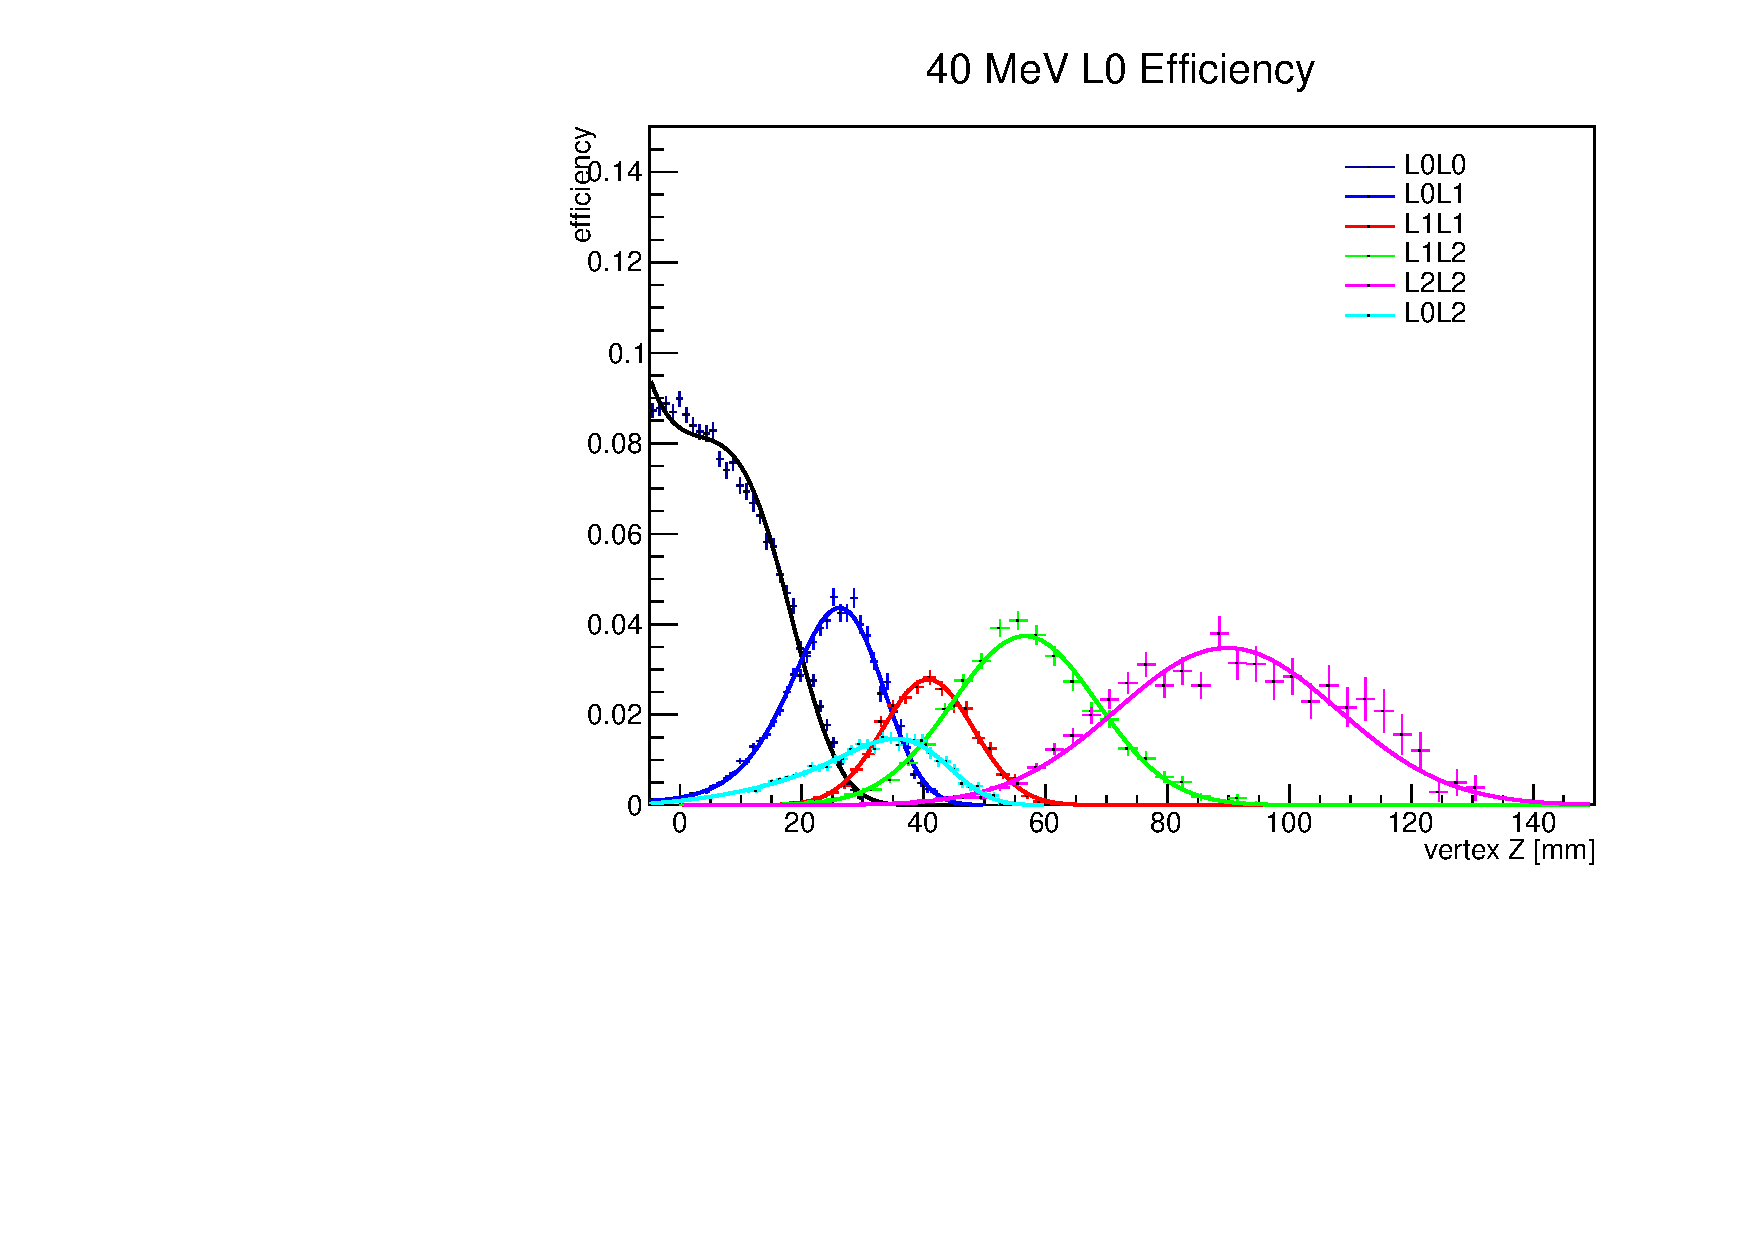
\includegraphics[width=0.55\linewidth]{figs/L0_eff_40.pdf}
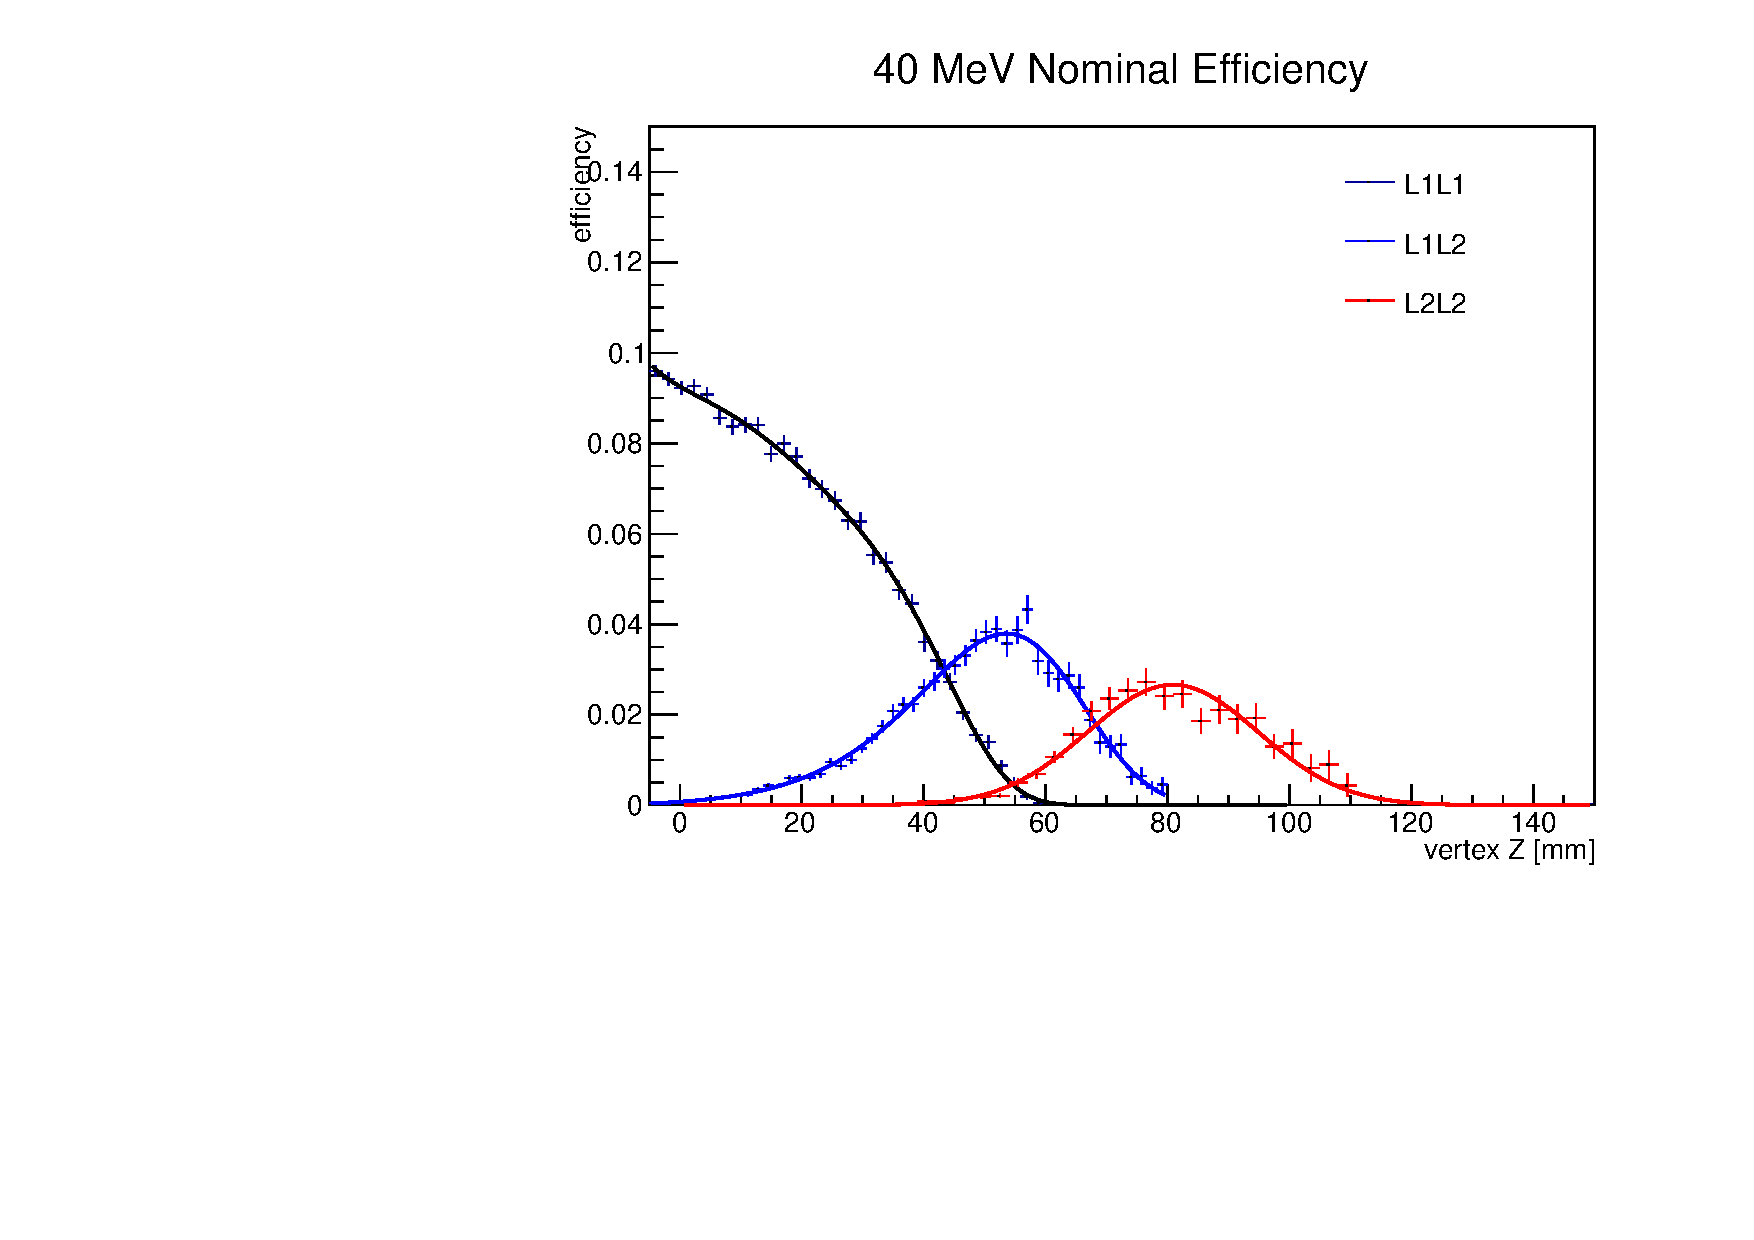
\includegraphics[width=0.55\linewidth]{figs/nominal_eff_40.pdf}
\end{figure}

\end{frame}

%------------------------------------------------

\begin{frame}
\frametitle{Long-lived A' Efficiency Improvement (cont.)}
\begin{itemize}
\item Total efficiency sums efficiency of exclusive layer requirements
\end{itemize}
\begin{figure}
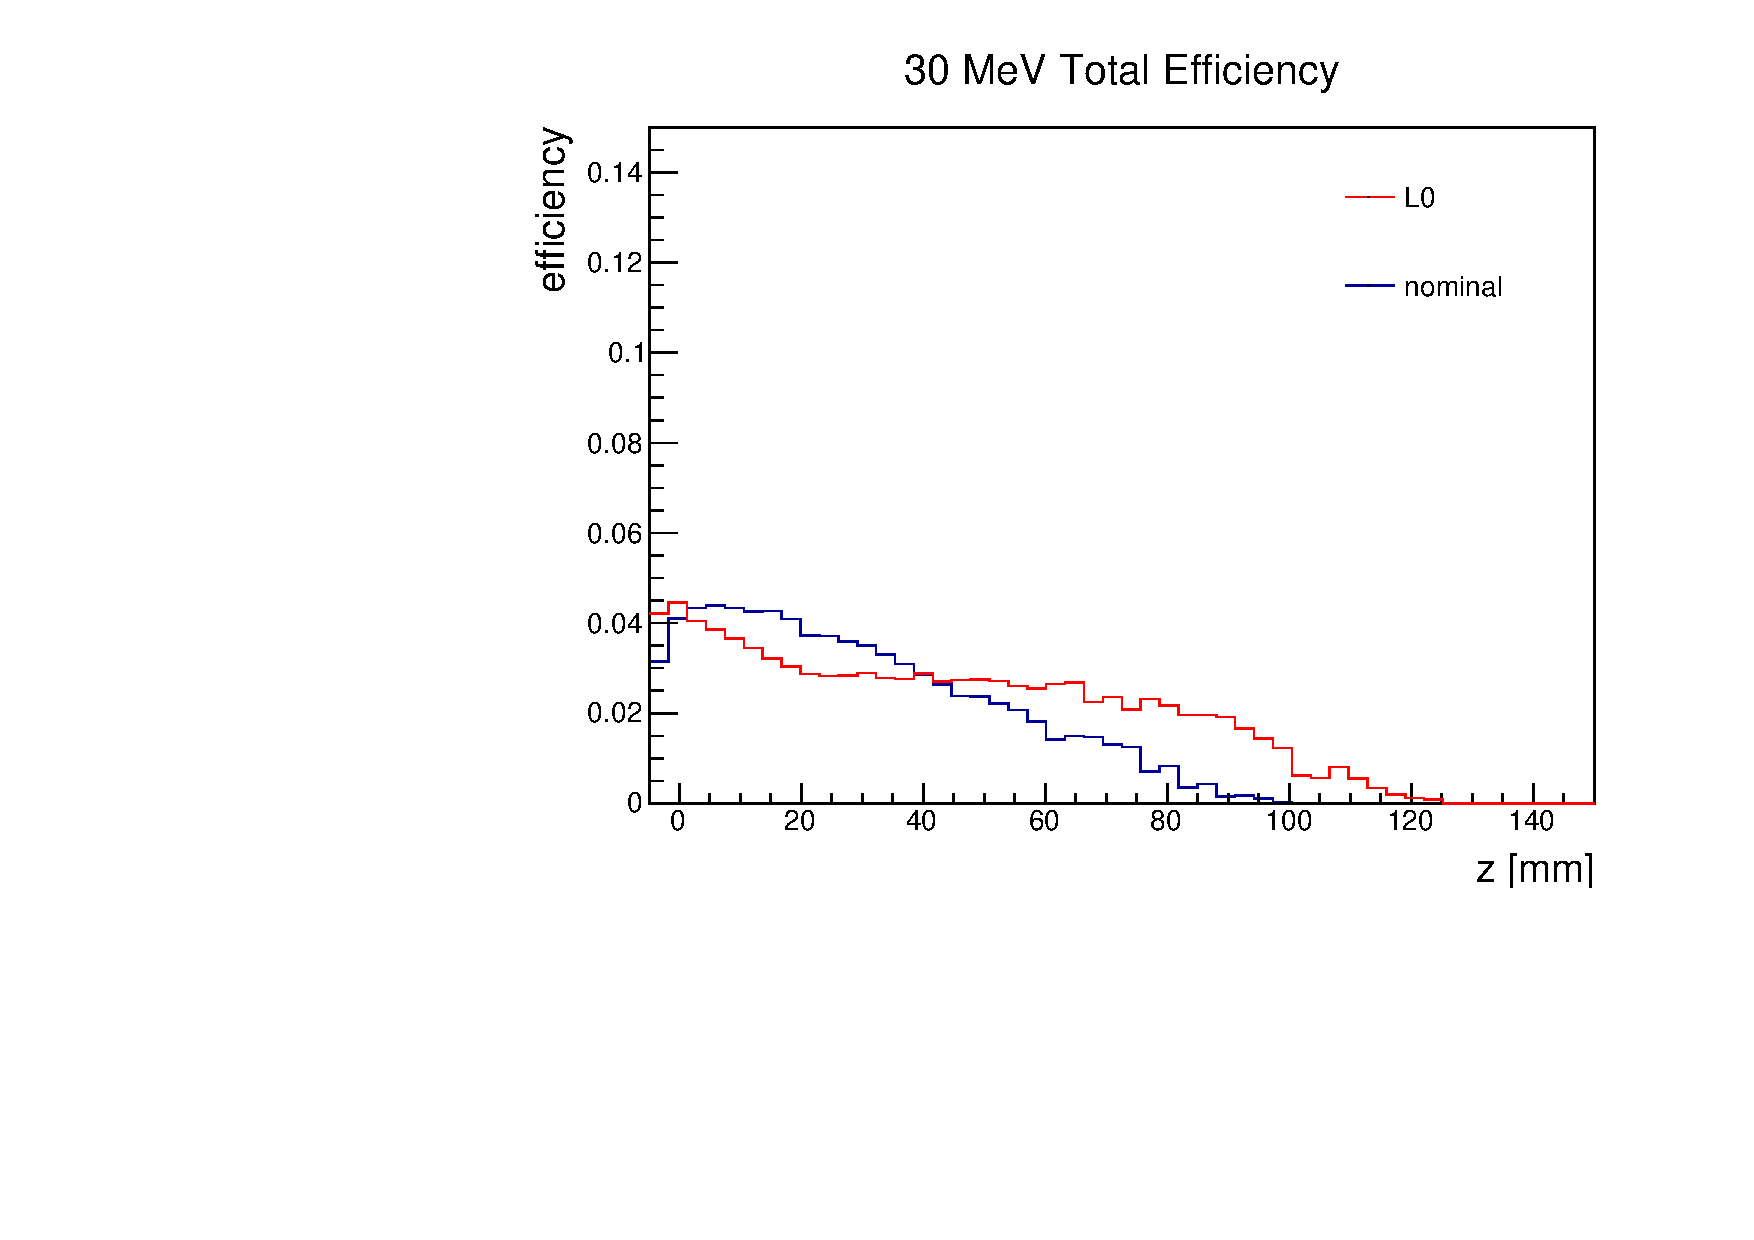
\includegraphics[width=0.38\linewidth]{figs/stat_eff_30loose_histo.pdf}
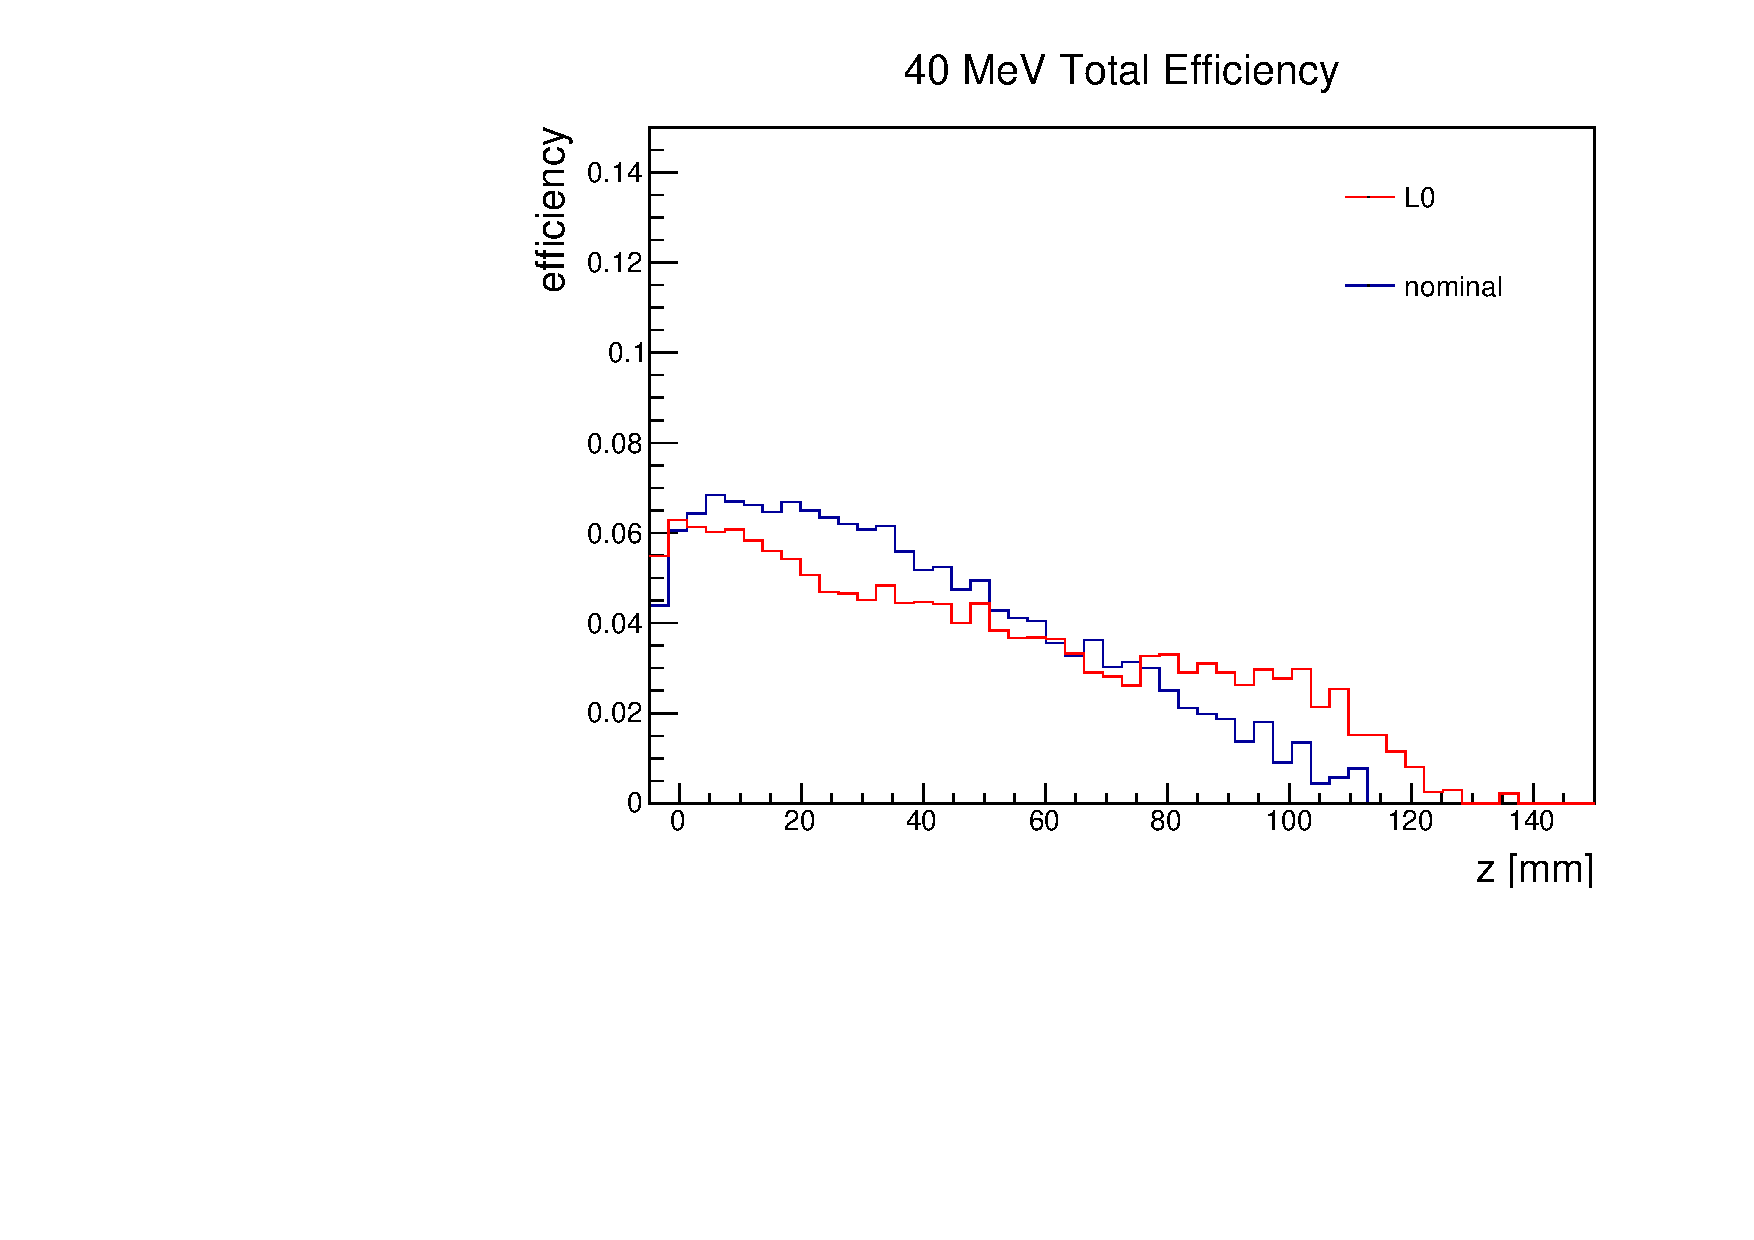
\includegraphics[width=0.38\linewidth]{figs/stat_eff_40loose_histo.pdf}
\end{figure}
\begin{figure}
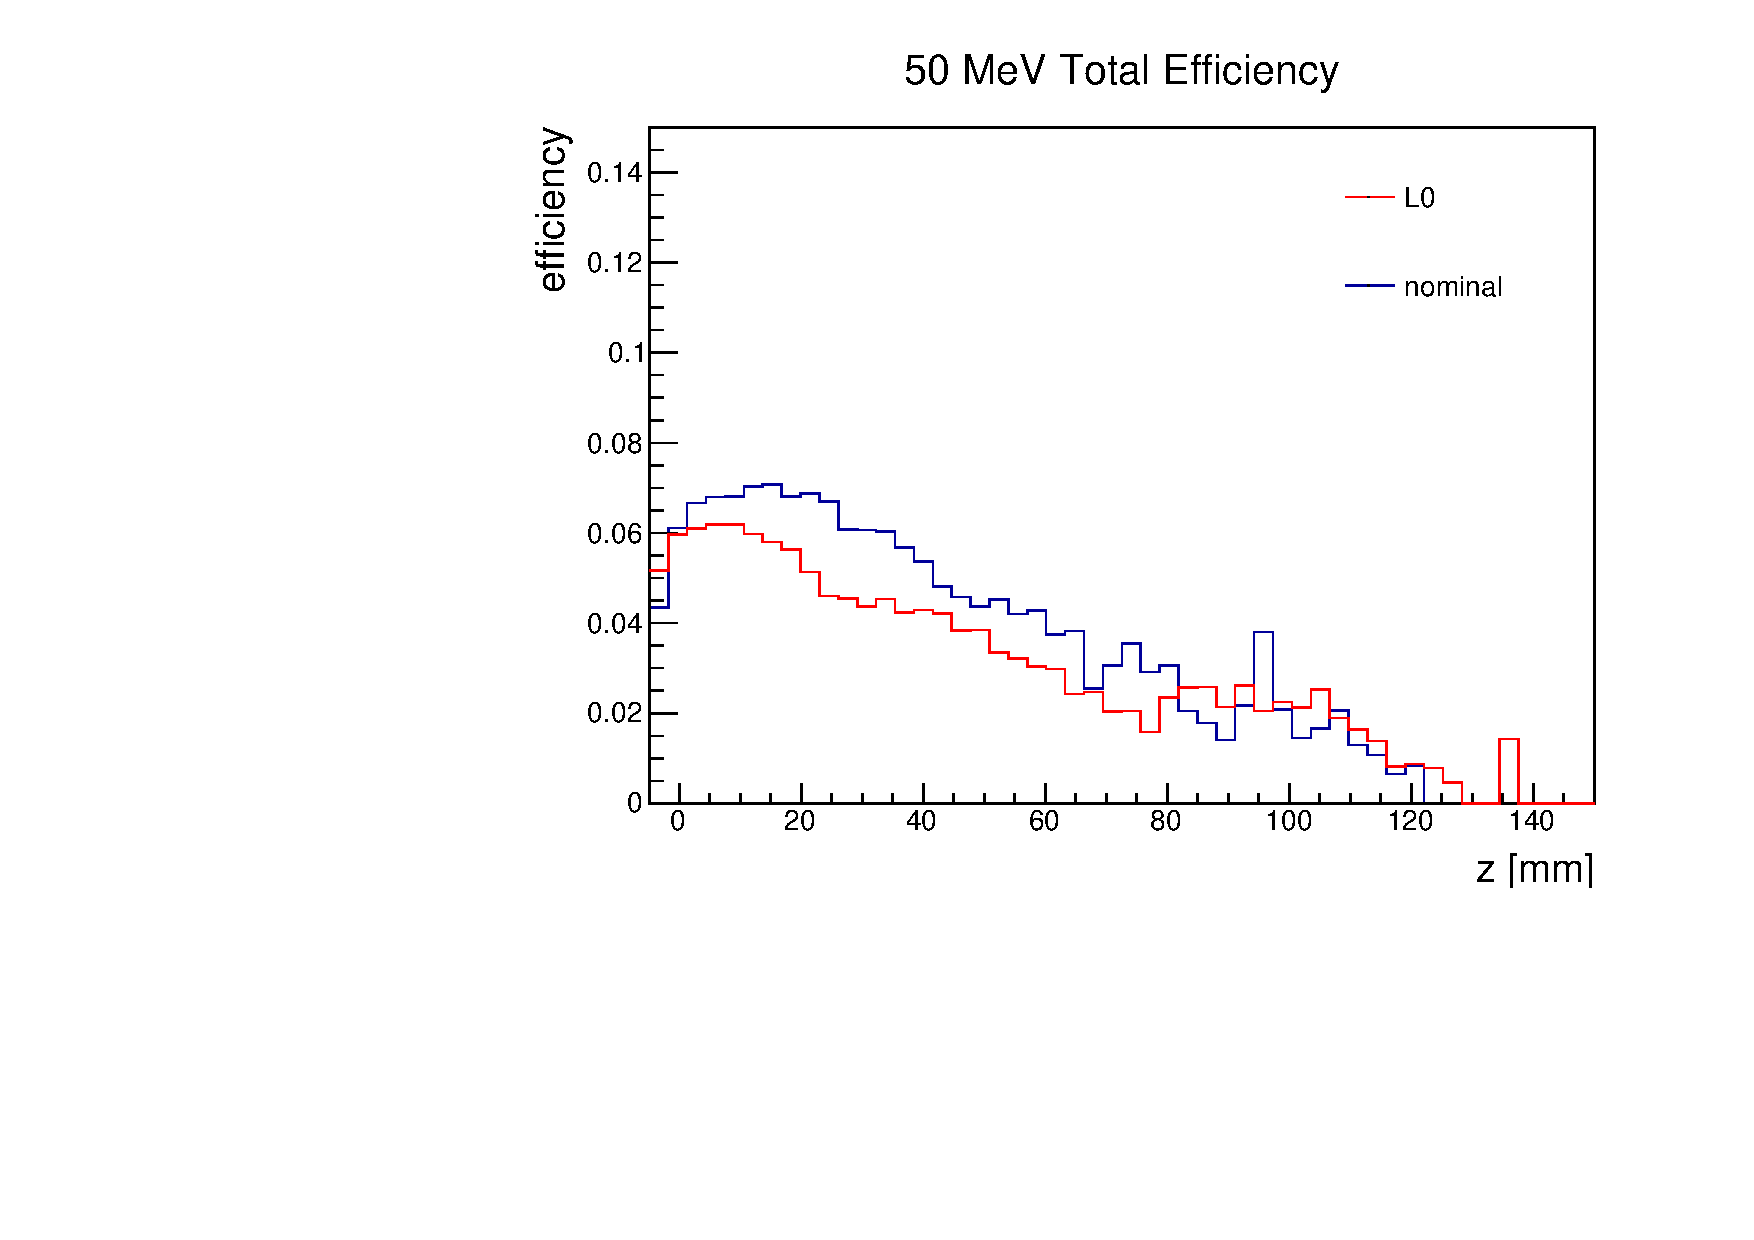
\includegraphics[width=0.38\linewidth]{figs/stat_eff_50loose_histo.pdf}
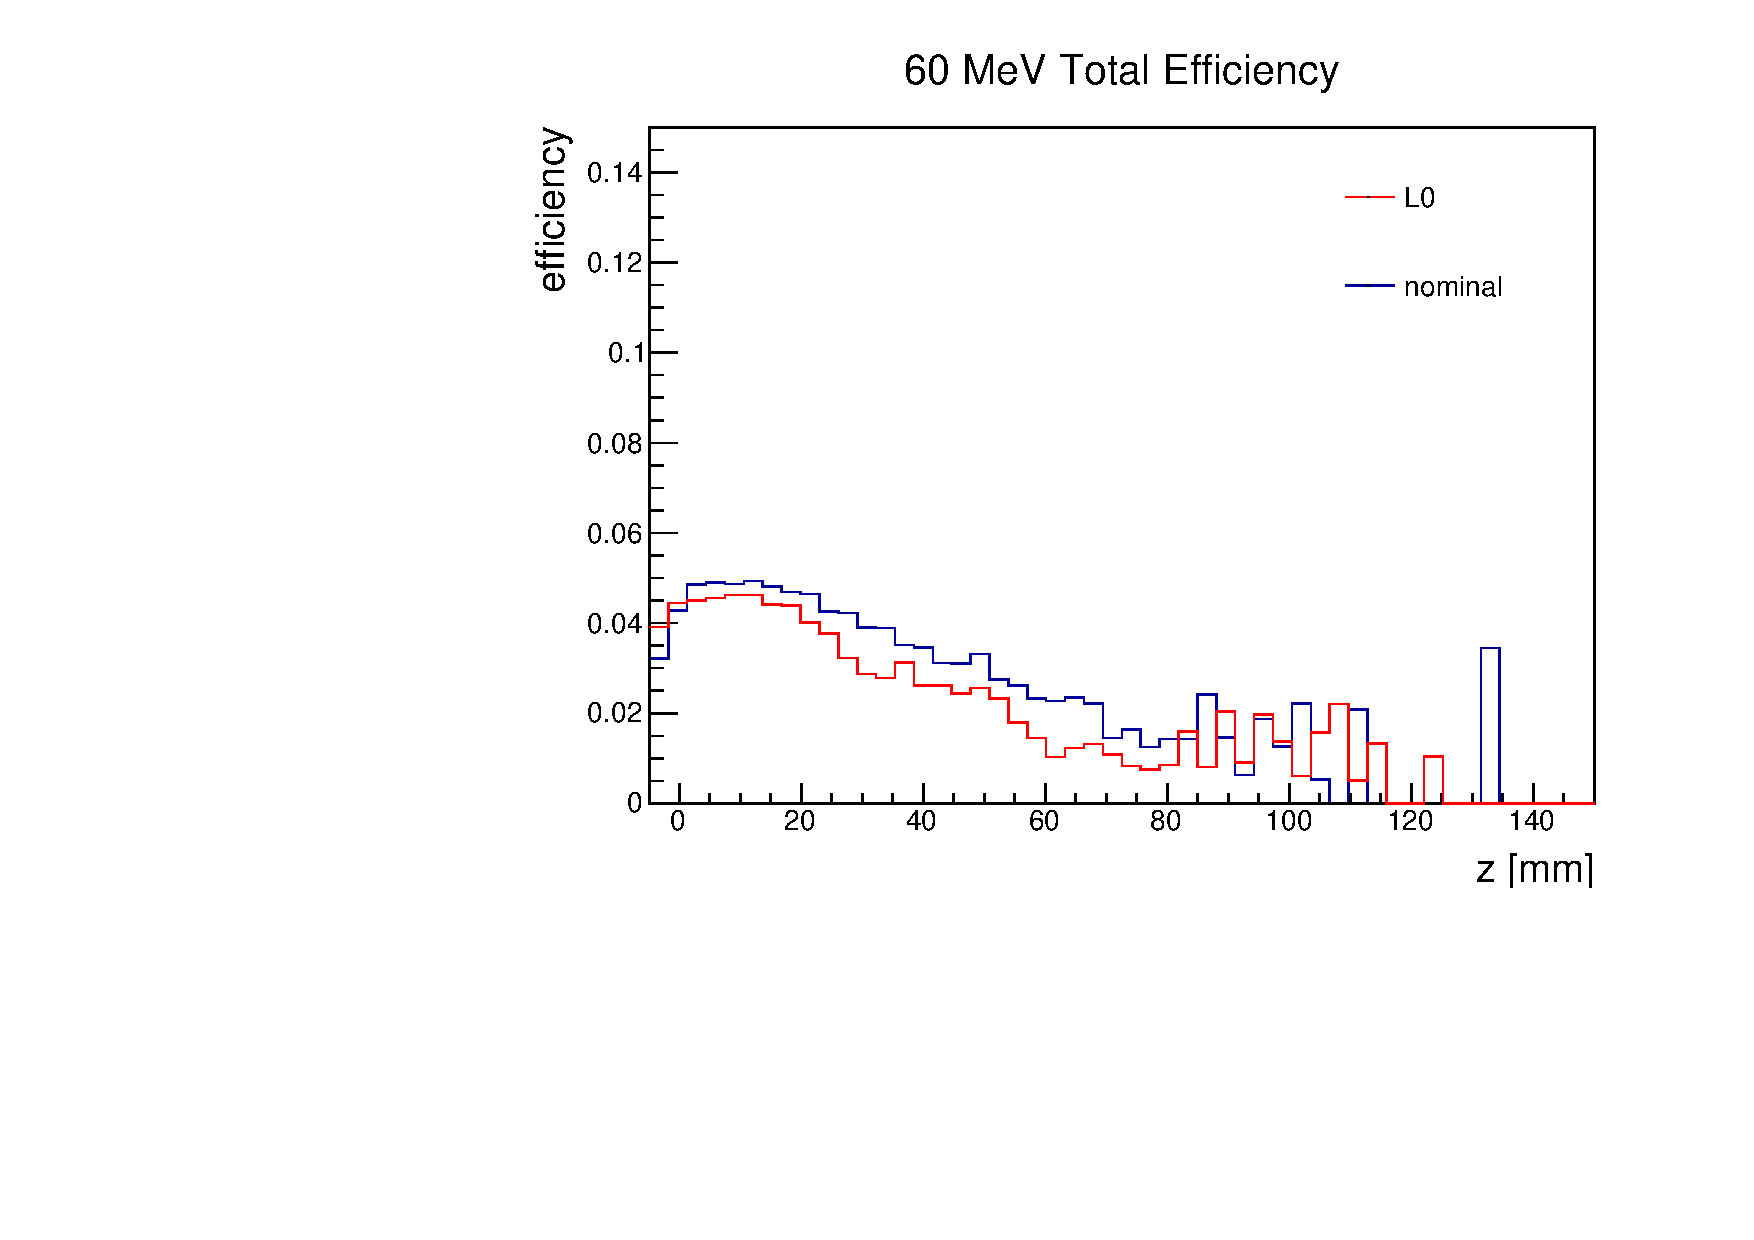
\includegraphics[width=0.38\linewidth]{figs/stat_eff_60loose_histo.pdf}
\end{figure}

\end{frame}

%------------------------------------------------

\begin{frame}
\frametitle{Vertex Resolution Improvement}
\begin{itemize}
\item \textcolor{darkgray}{\textbf{Vertex resolution improves by about a factor of 2}} for 1.05 GeV(dependent on mass and beam energy)
\end{itemize}
\begin{figure}
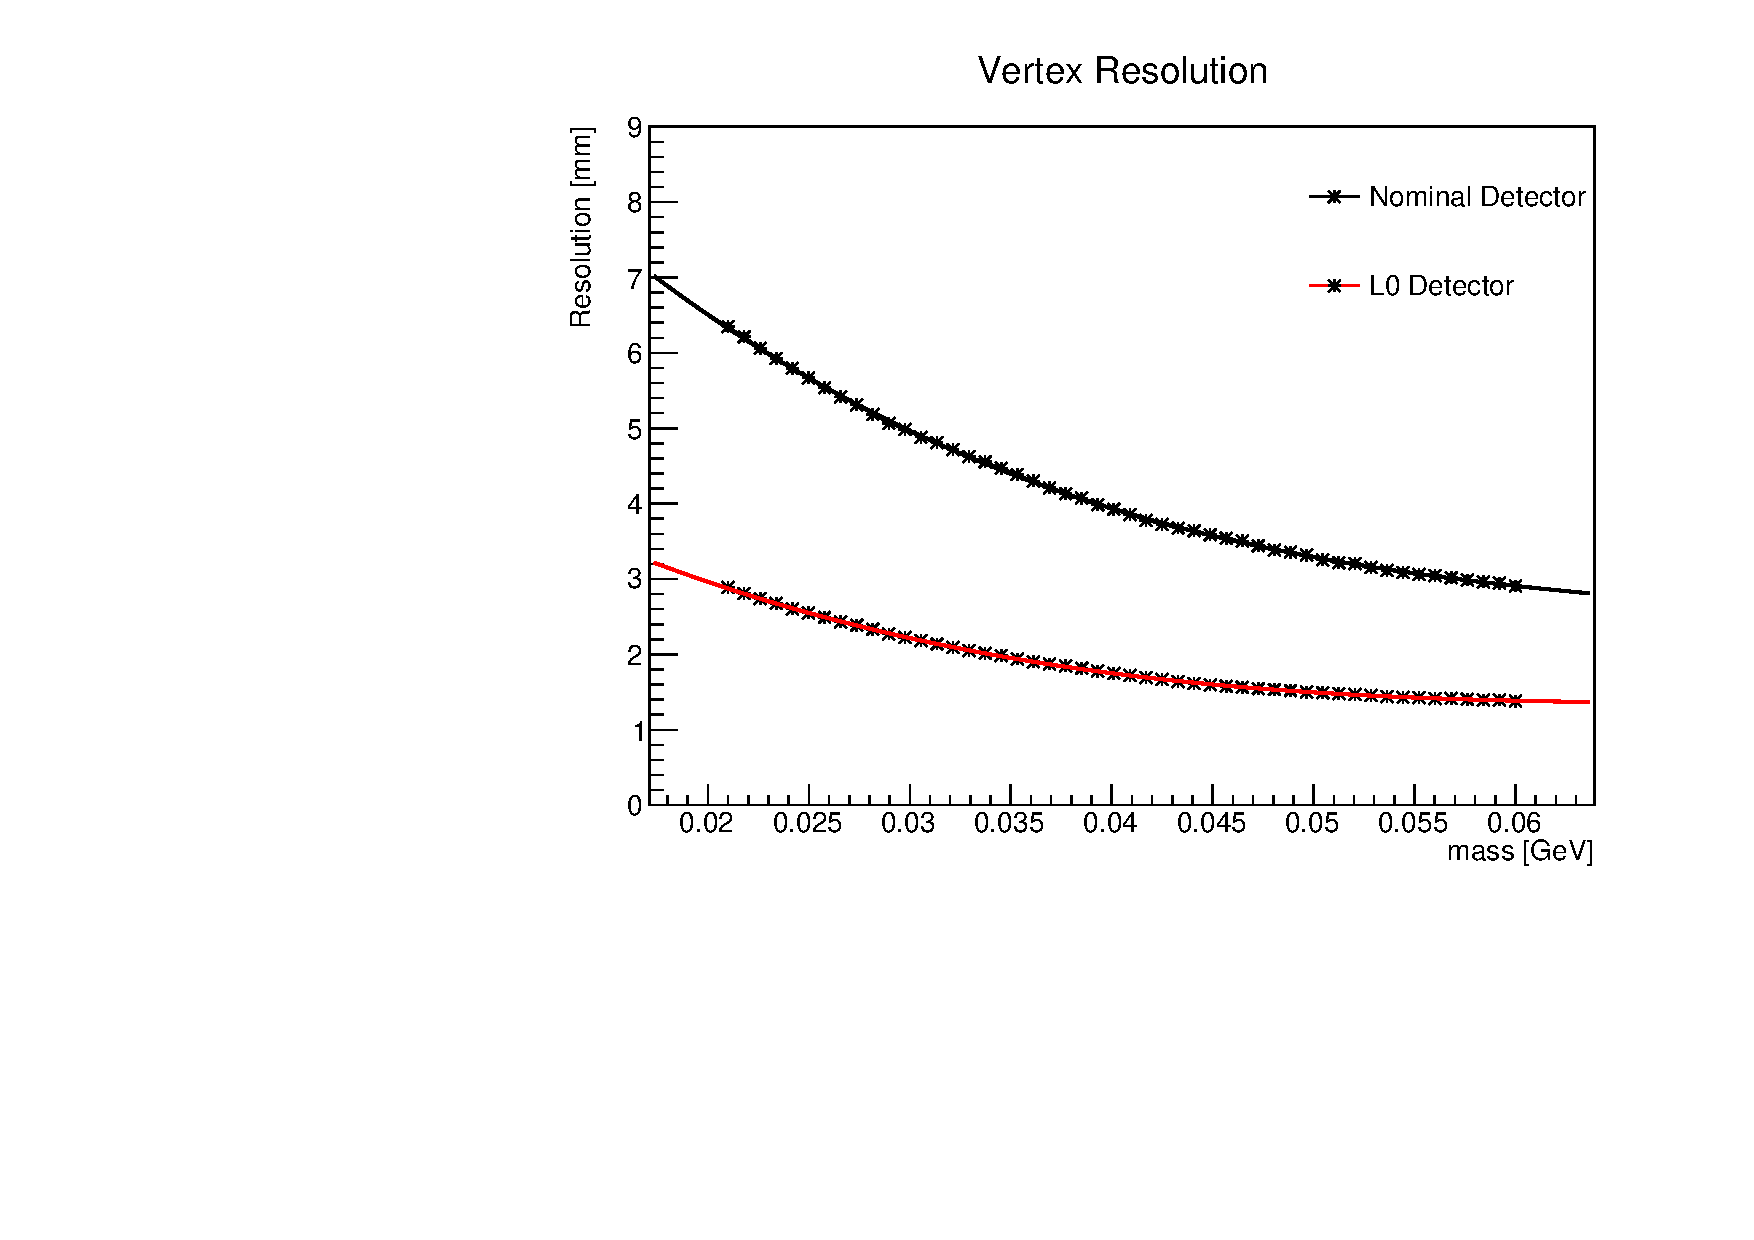
\includegraphics[width=0.6\linewidth]{figs/VZ_Resolution_1pt05.pdf}
\end{figure}

\end{frame}

%------------------------------------------------

\begin{frame}
\frametitle{Vertex Resolution Improvement All Energies}
\begin{itemize}
\item Background are dominated by multiple scattering which decreases with increasing momentum
\item L0 vertex resolution improvement decreases slightly with increasing beam energy (still a very good improvement!)
\end{itemize}
\begin{figure}
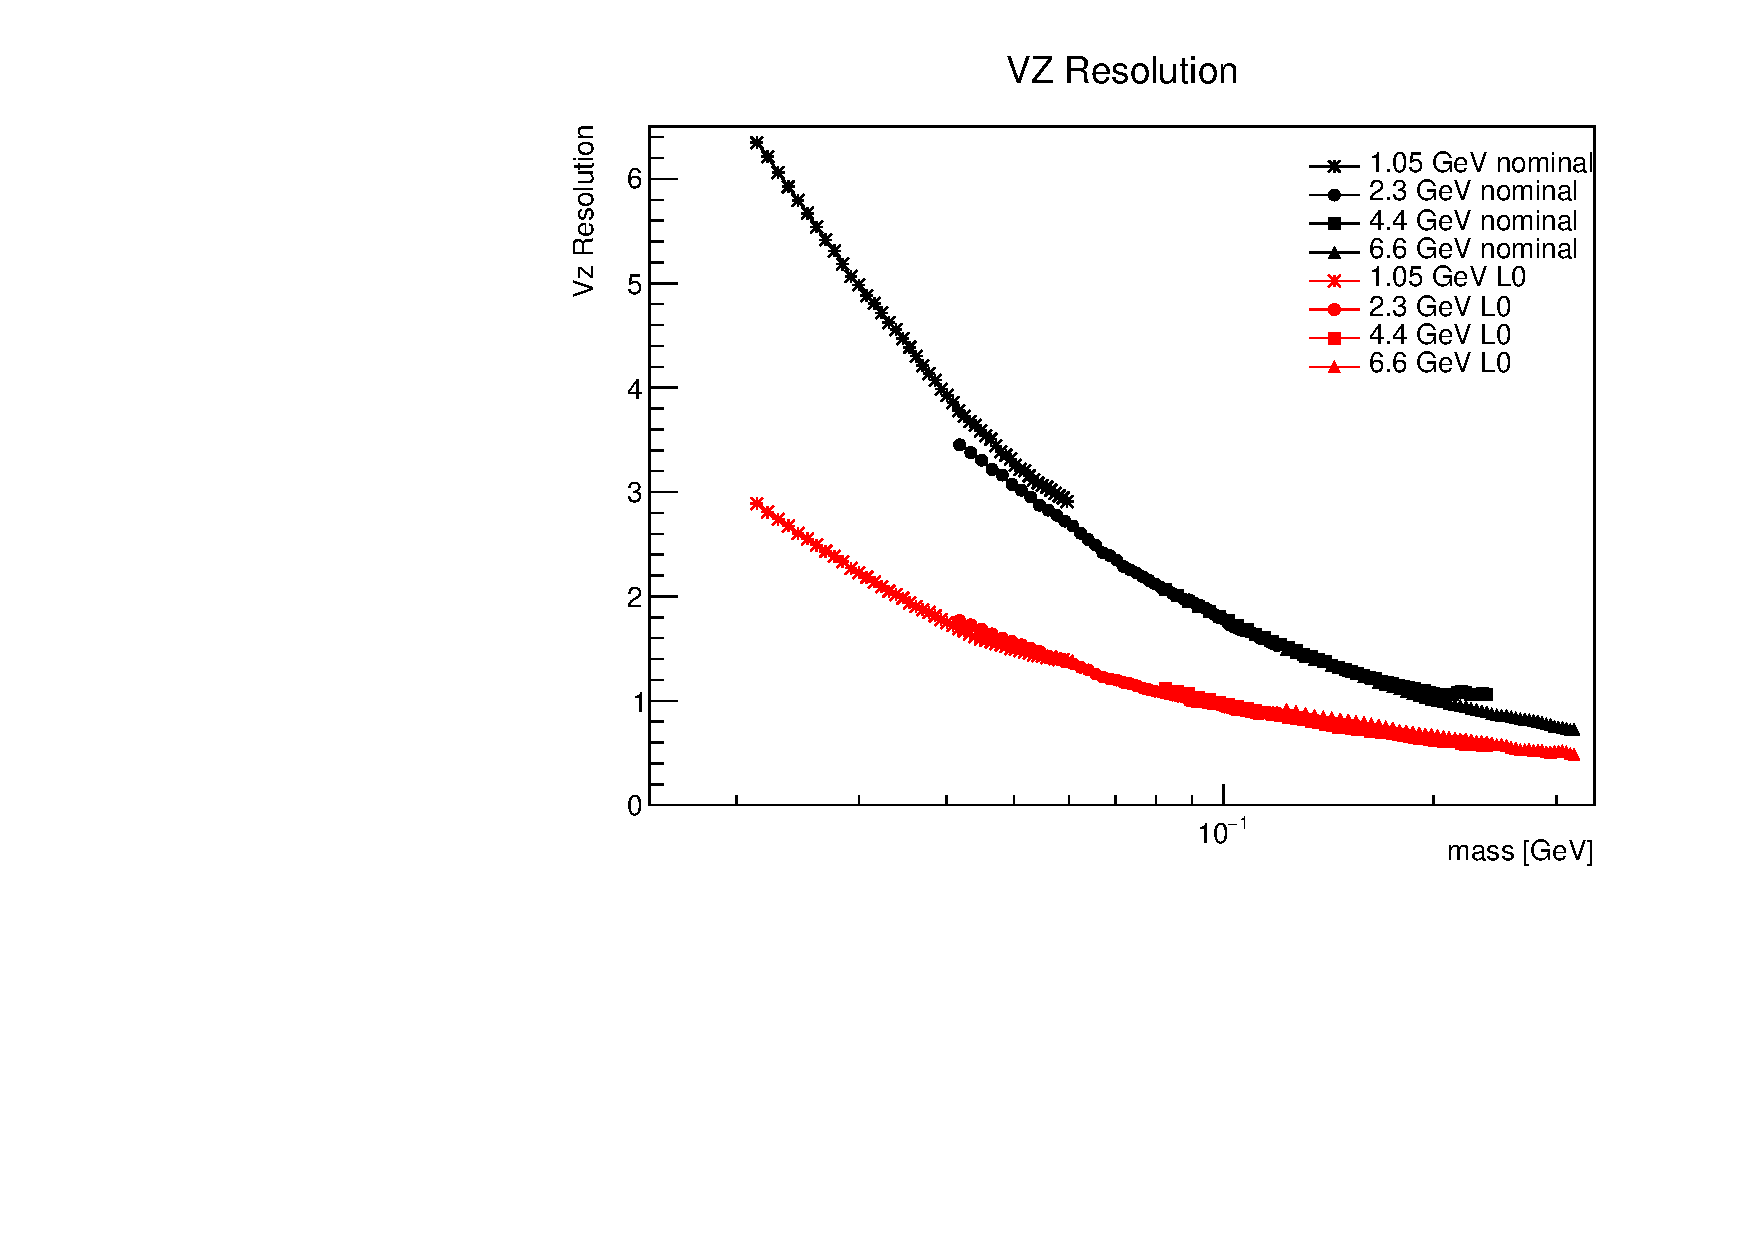
\includegraphics[width=0.55\linewidth]{figs/VZ_Resolution_total.pdf}
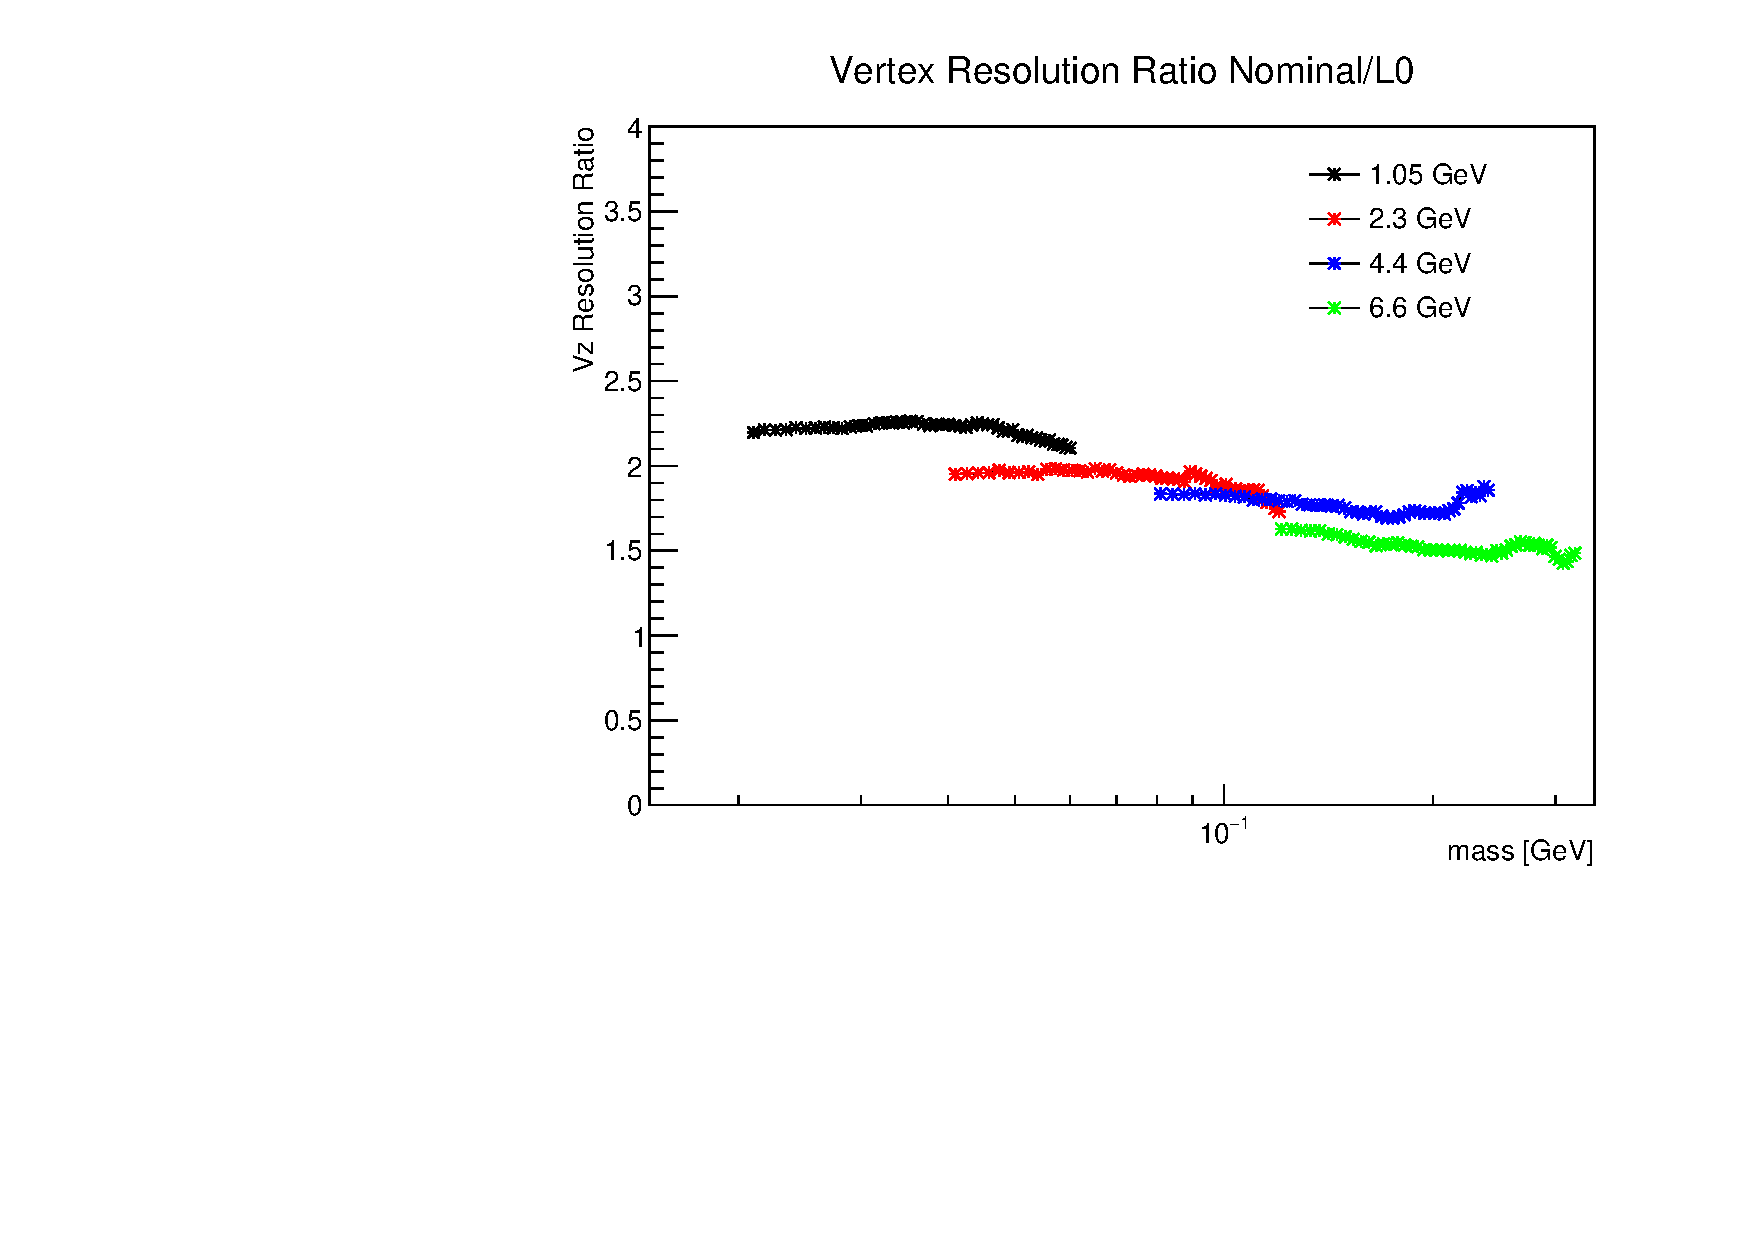
\includegraphics[width=0.55\linewidth]{figs/VZ_Resolution_ratio.pdf}
\end{figure}

\end{frame}

%------------------------------------------------

\begin{frame}
\frametitle{Improved Z Cuts}
\begin{itemize}
\item Improved vertex resolution causes \textcolor{darkgray}{\textbf{improved z cuts}} (by about the same factor)
\item Z cuts for L0 (left) and nominal (right) at various luminosities
\end{itemize}
\begin{figure}
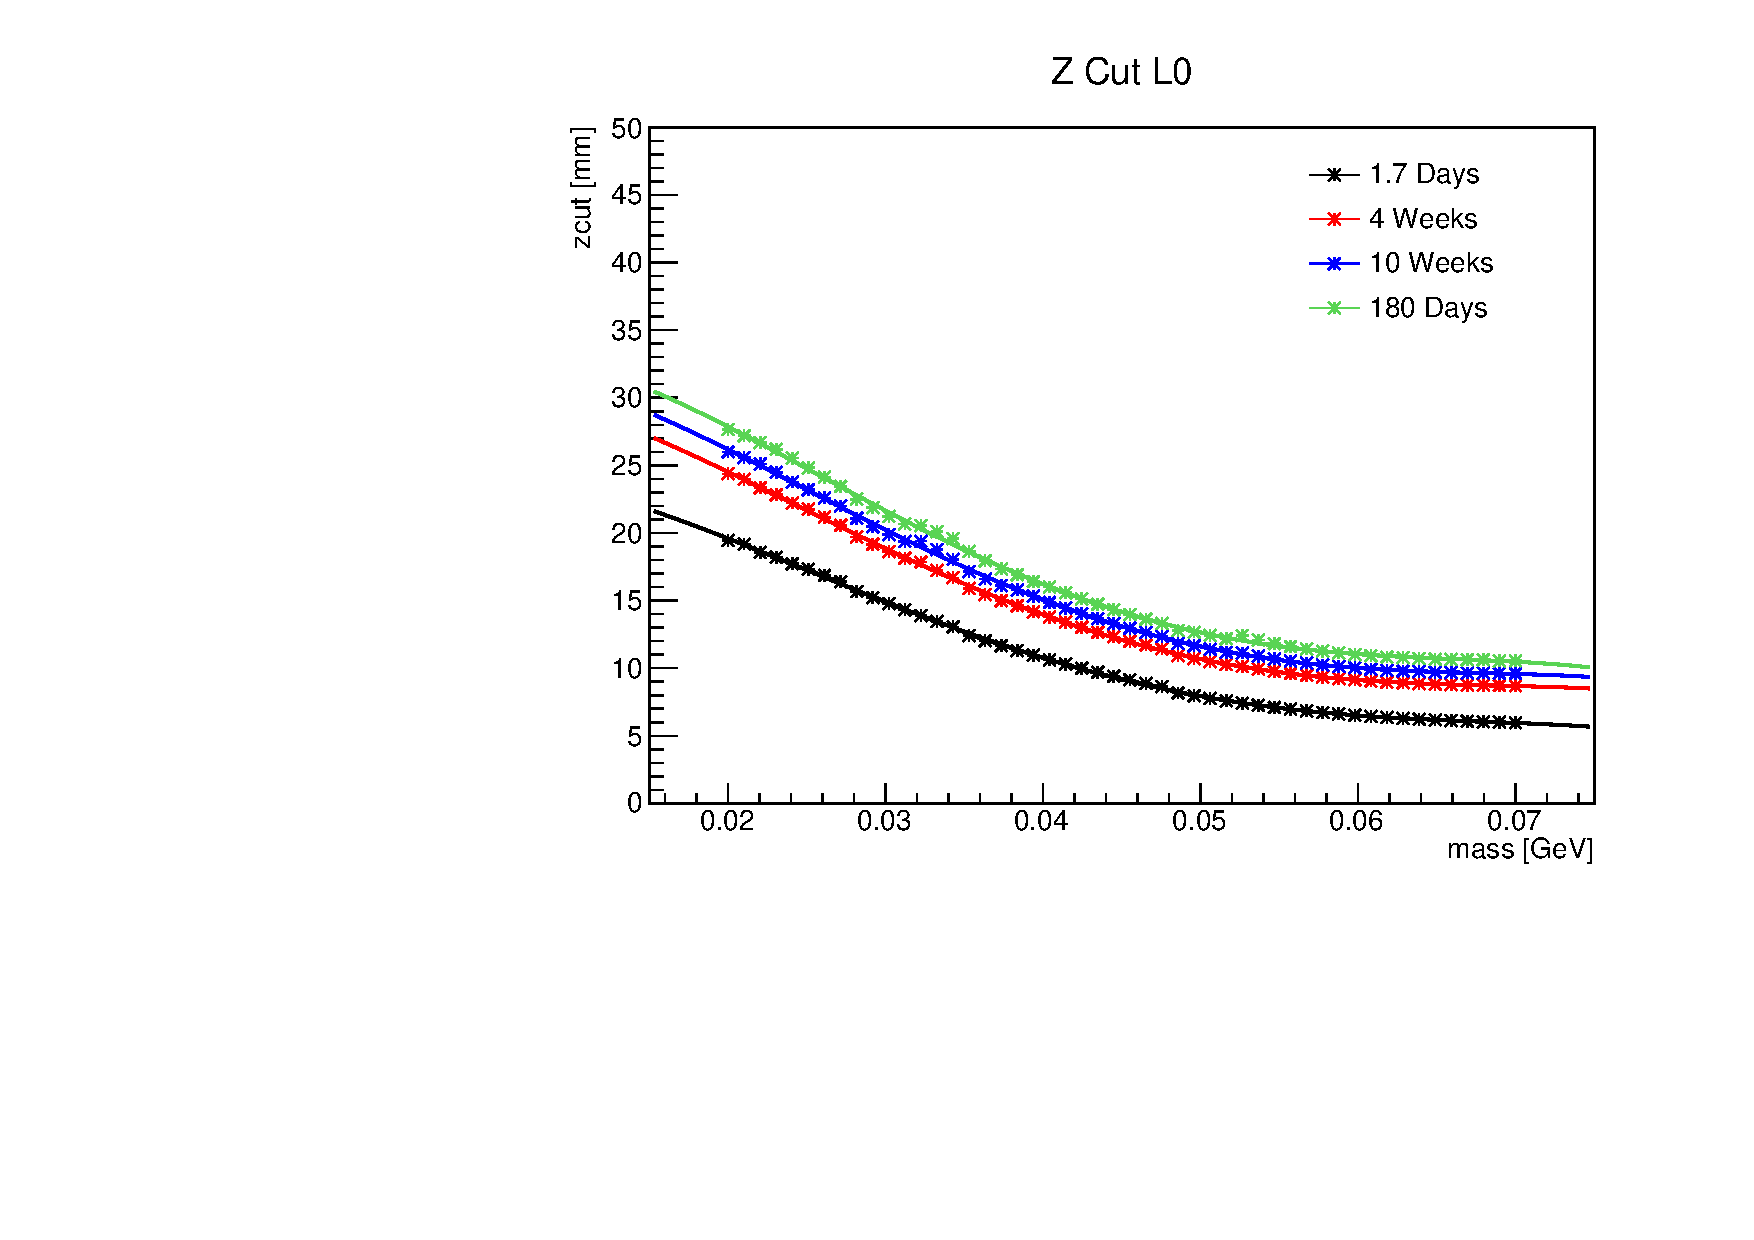
\includegraphics[width=0.55\linewidth]{figs/zcut_L0_loose.pdf}
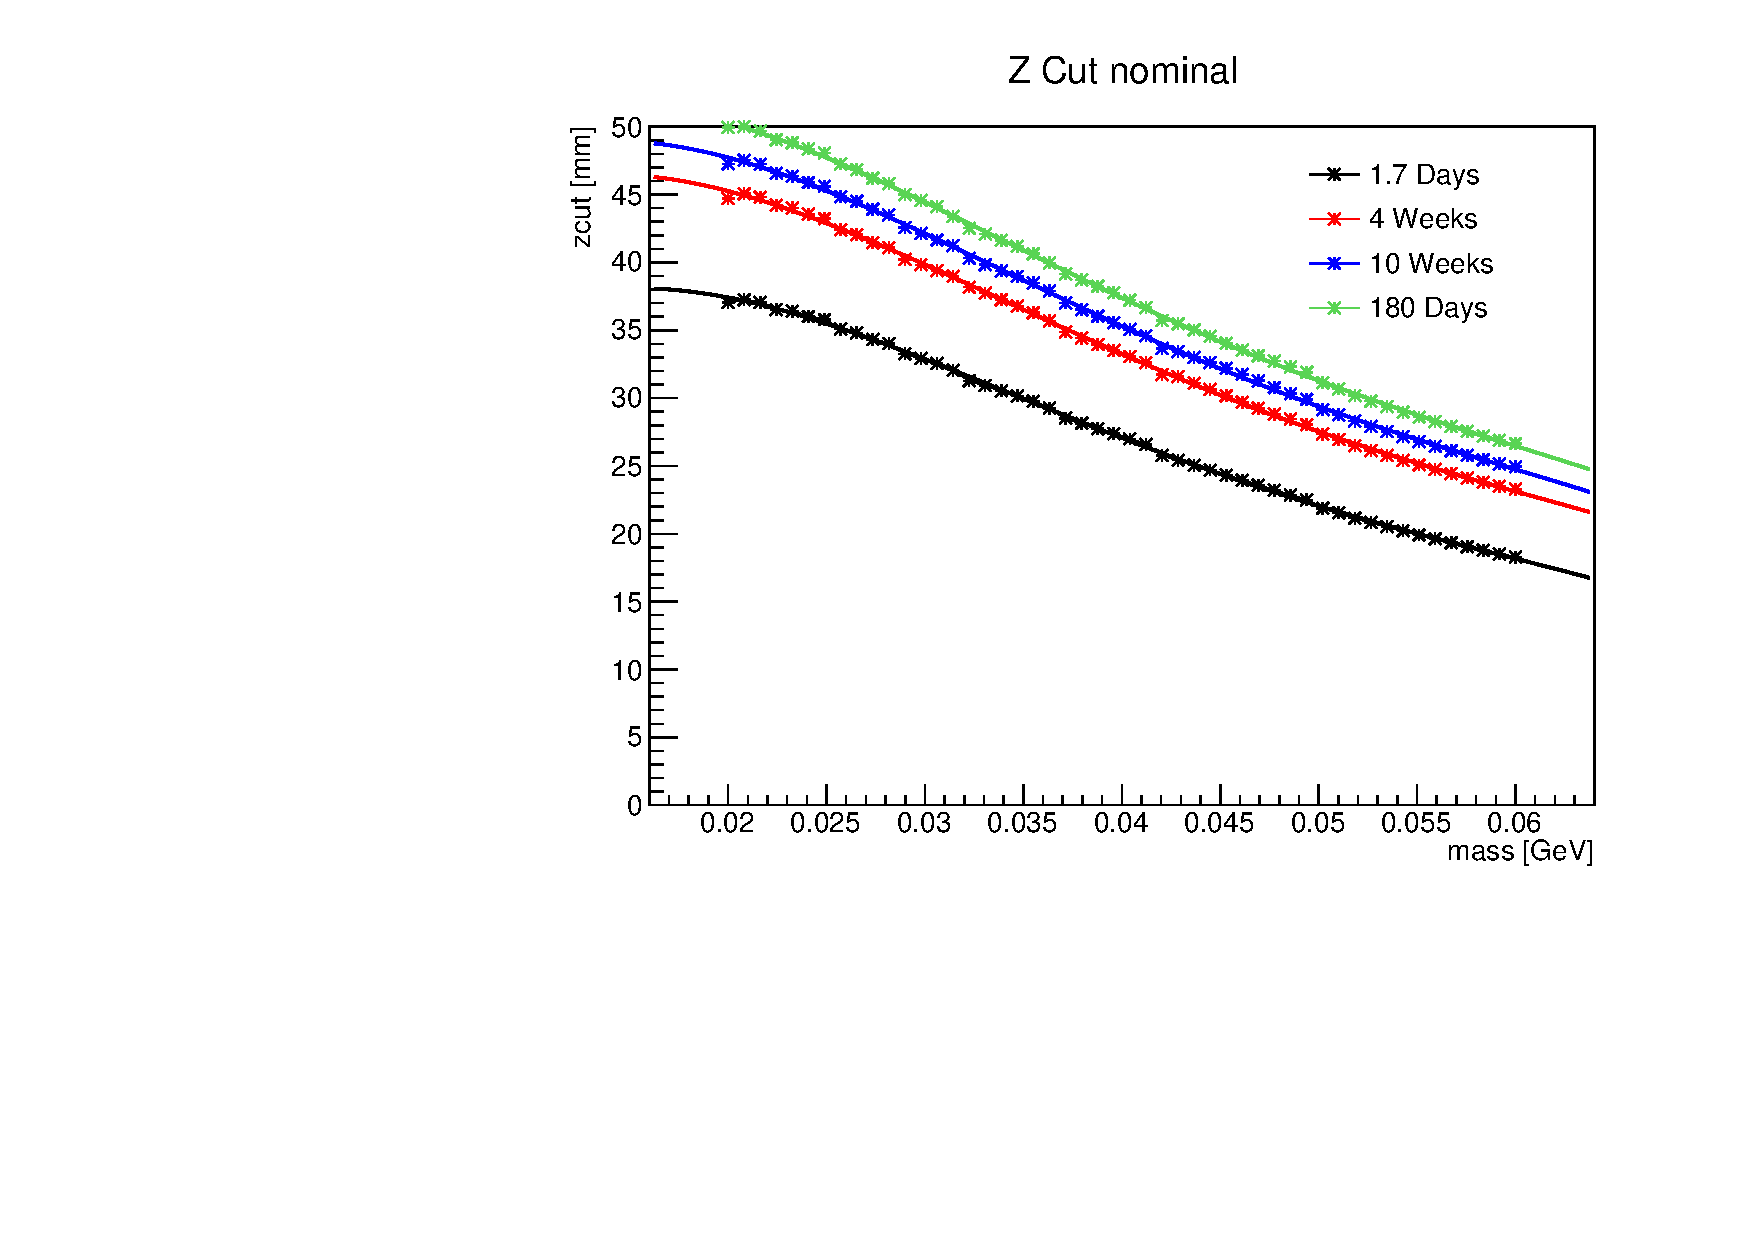
\includegraphics[width=0.55\linewidth]{figs/zcut_nominal.pdf}
\end{figure}

\end{frame}

%------------------------------------------------

\begin{frame}
\frametitle{Effect of Improved Z Cut}
\begin{itemize}
\item A' decays are exponential in $z$, so the \textcolor{darkgray}{\textbf{number of detectable A's increases dramatically}} for lower Z Cut
\item Efficiency after cuts and acceptance with z cuts (left), produced A's (right)
\end{itemize}
\begin{figure}
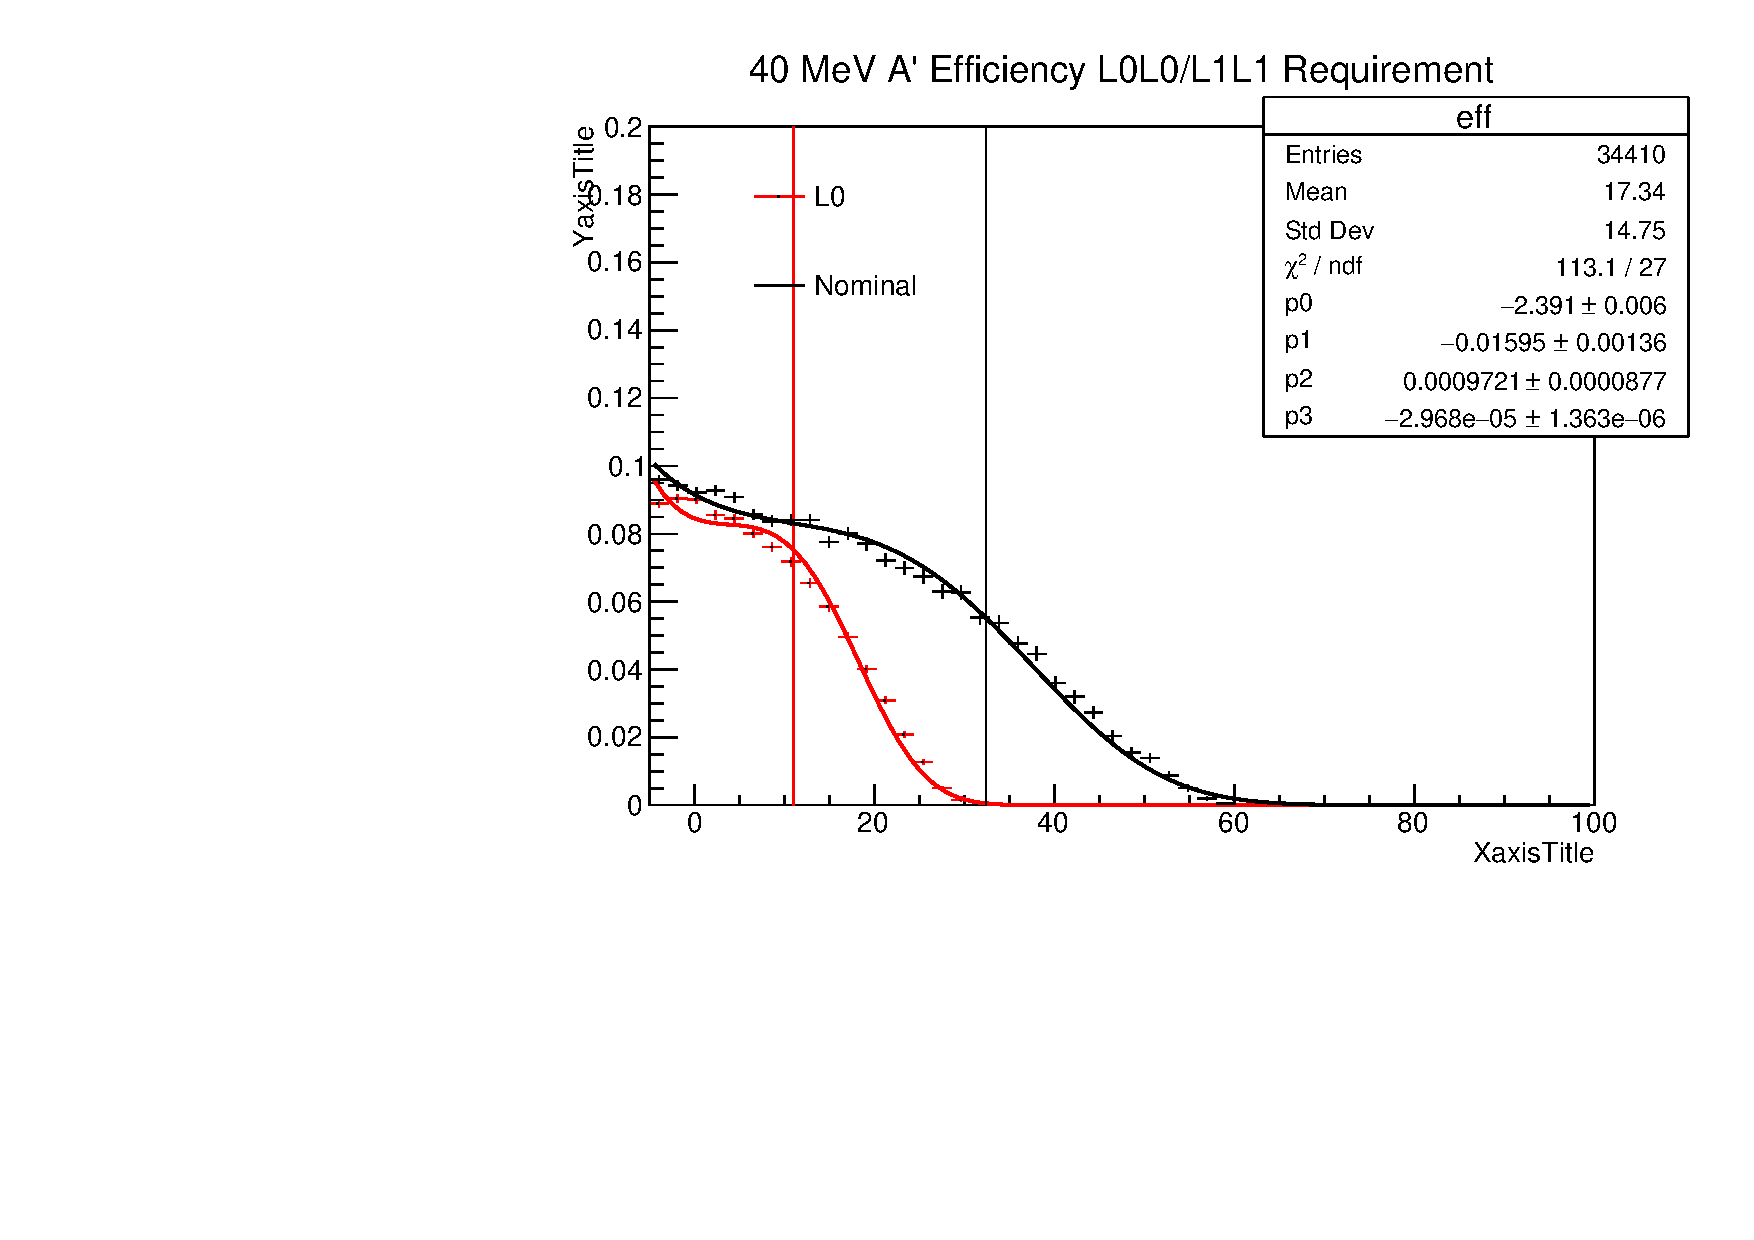
\includegraphics[width=0.55\linewidth]{figs/eff_40.pdf}
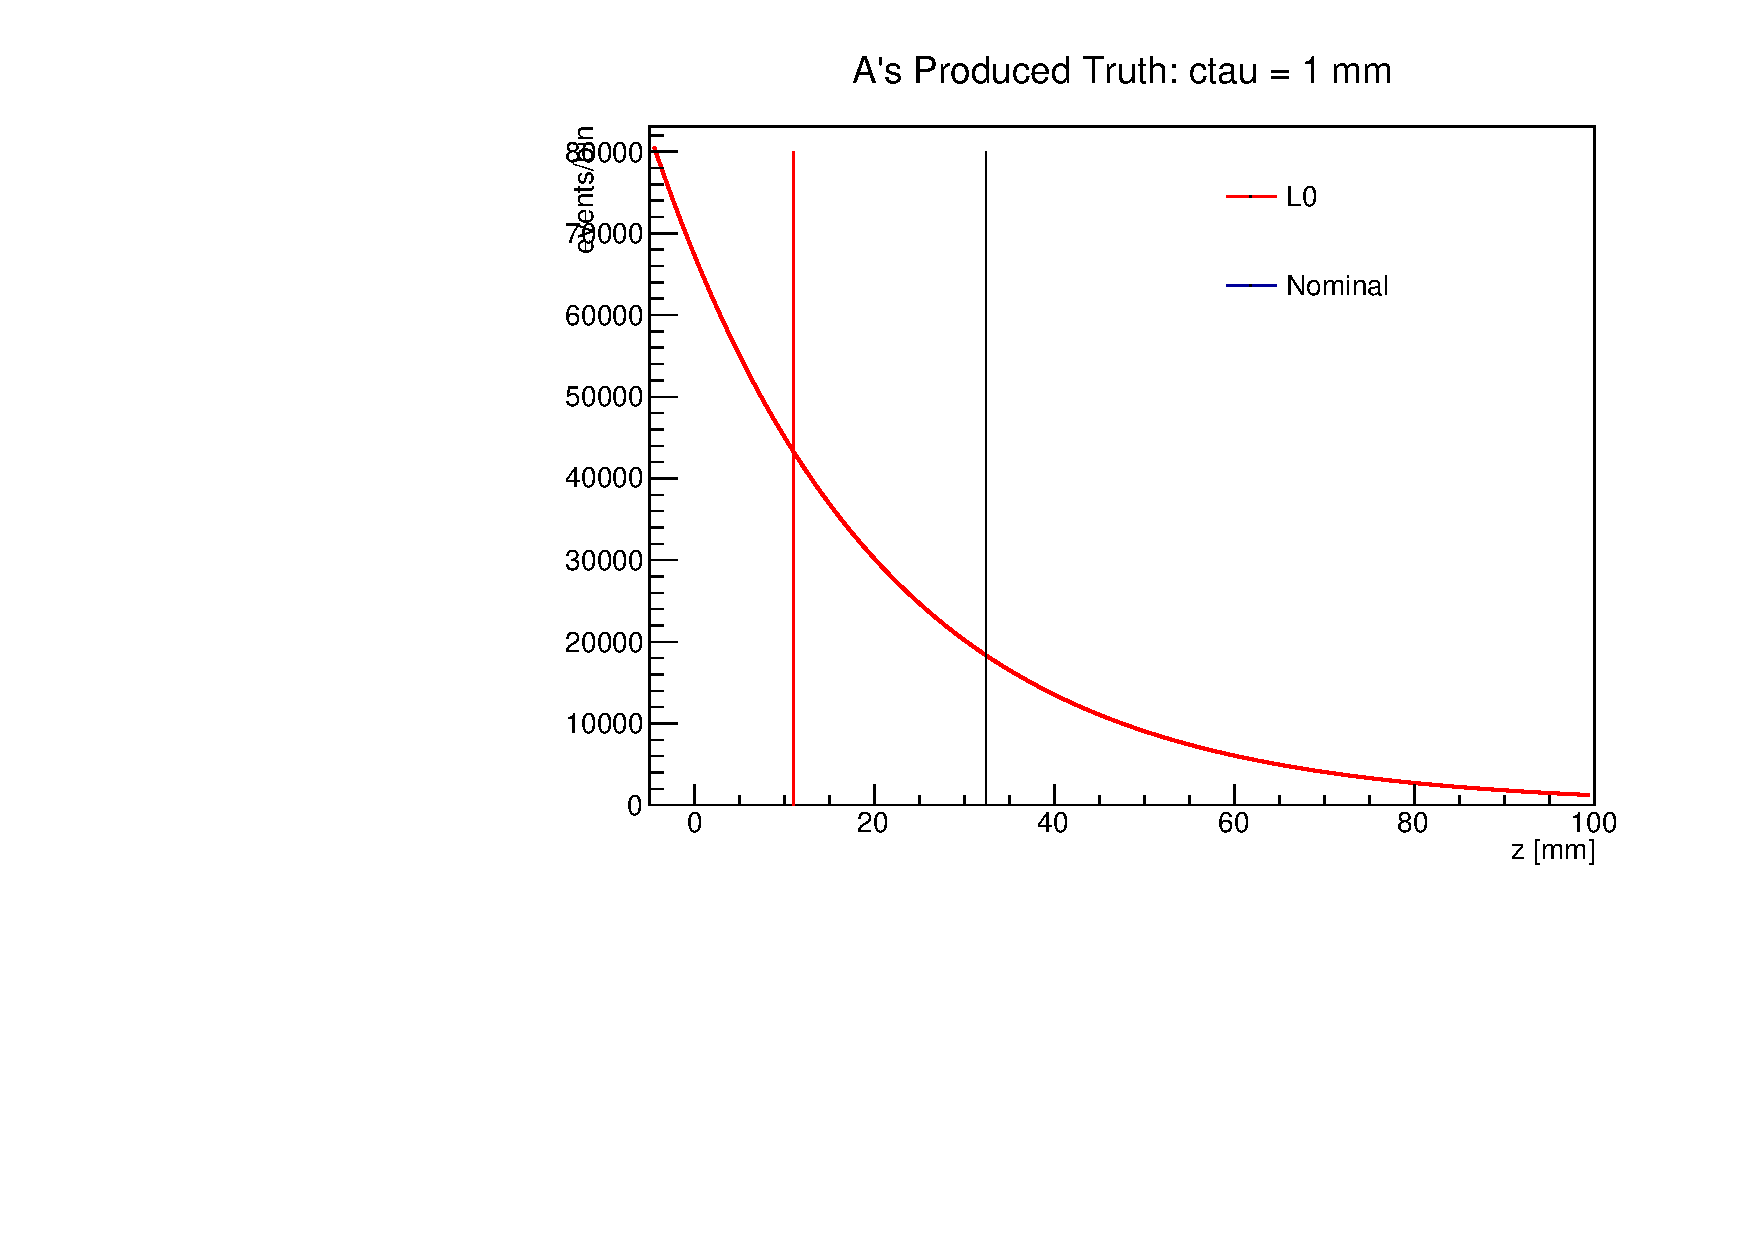
\includegraphics[width=0.55\linewidth]{figs/ap_produced.pdf}
\end{figure}

\end{frame}

%------------------------------------------------

\begin{frame}
\frametitle{Procedure for Obtaining Reach - Determining Z Cuts}
\begin{itemize}
\item Fit function $B(z)$ to tritrig distribution after cuts (Gaussian with non-Gaussian tail)
\item Scale function for desired luminosity, z cut is where $B(z)=0.5$ events in a mass bin of 2.6 times mass resolution
\end{itemize}
\begin{figure}
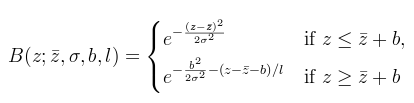
\includegraphics[width=0.35\linewidth]{figs/function.png}
\end{figure}
\begin{figure}
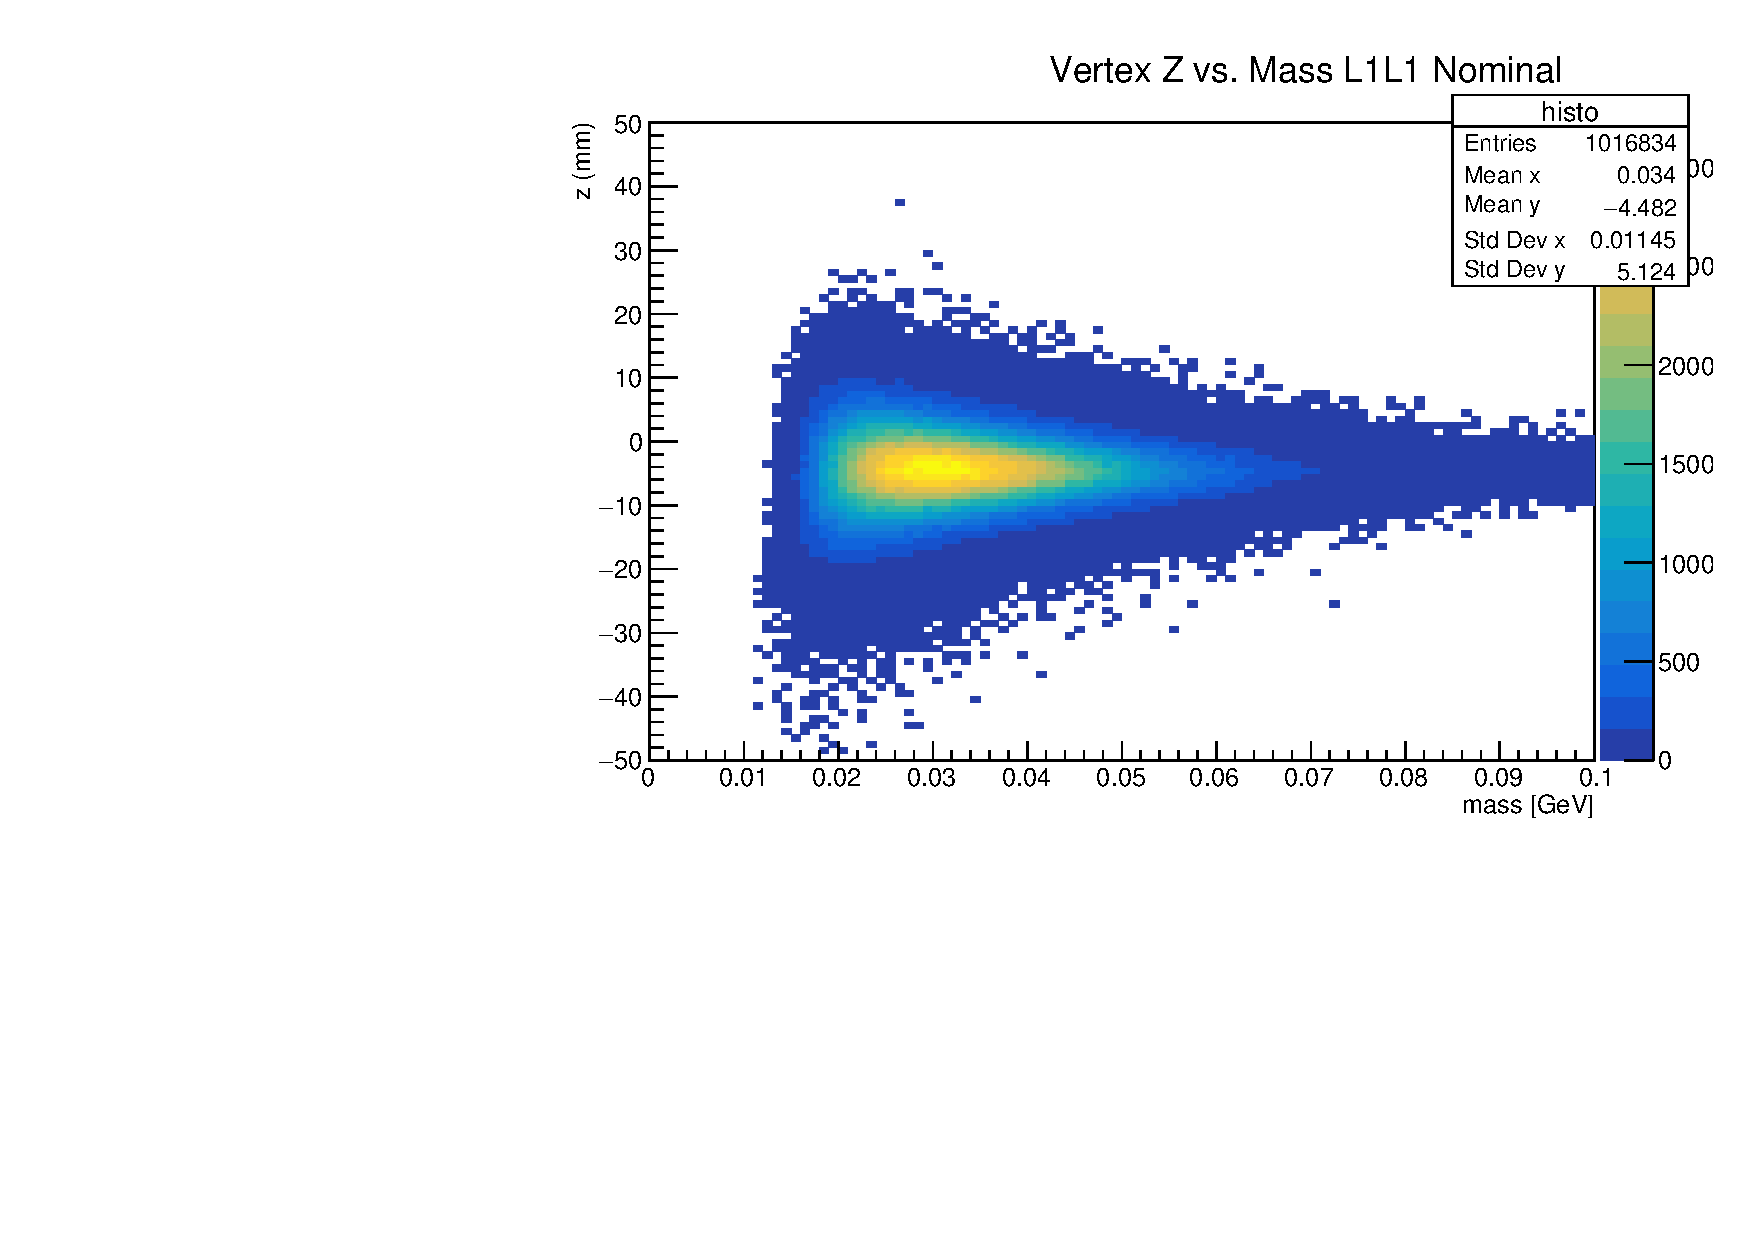
\includegraphics[width=0.45\linewidth]{figs/L1L1_loose_nom.pdf}
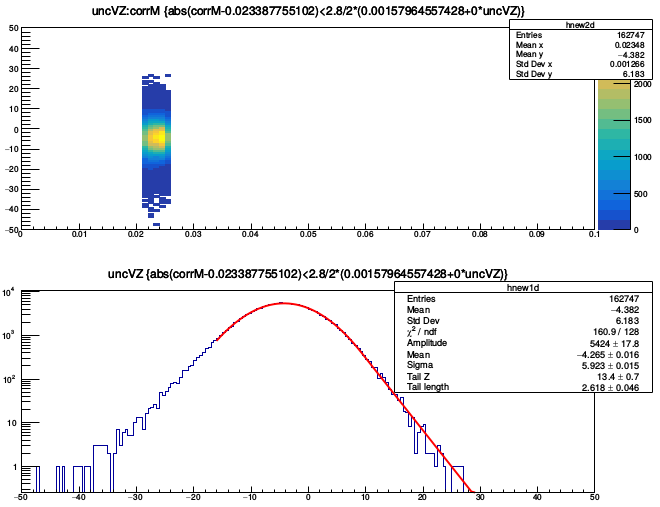
\includegraphics[width=0.4\linewidth]{figs/mass_slice.png}
\end{figure}

\end{frame}

%------------------------------------------------

\begin{frame}
\frametitle{Procedure for Obtaining Reach - Calculating Detectable A's}
\begin{equation}
\mu s(z) = (N_{A'} \epsilon_{reco} (z_{targ})) \frac{e^{\frac{z_{targ}-z}{\gamma c \tau}}}{\gamma c \tau} \frac{\epsilon_{reco}(z)}{\epsilon_{reco}(z_{targ})} \epsilon_{cut}(z)
\end{equation}
\begin{itemize}
\item Number of detectable events is simply $\int_{z_{cut}}^{z_{max}} \mu s(z) dz$ (essentially efficiency(z) * acceptance(z) * number of A's(z))
\item Reach contours are defined at the 90\% confidence level which is 2.3 expected events
\end{itemize}
\begin{figure}
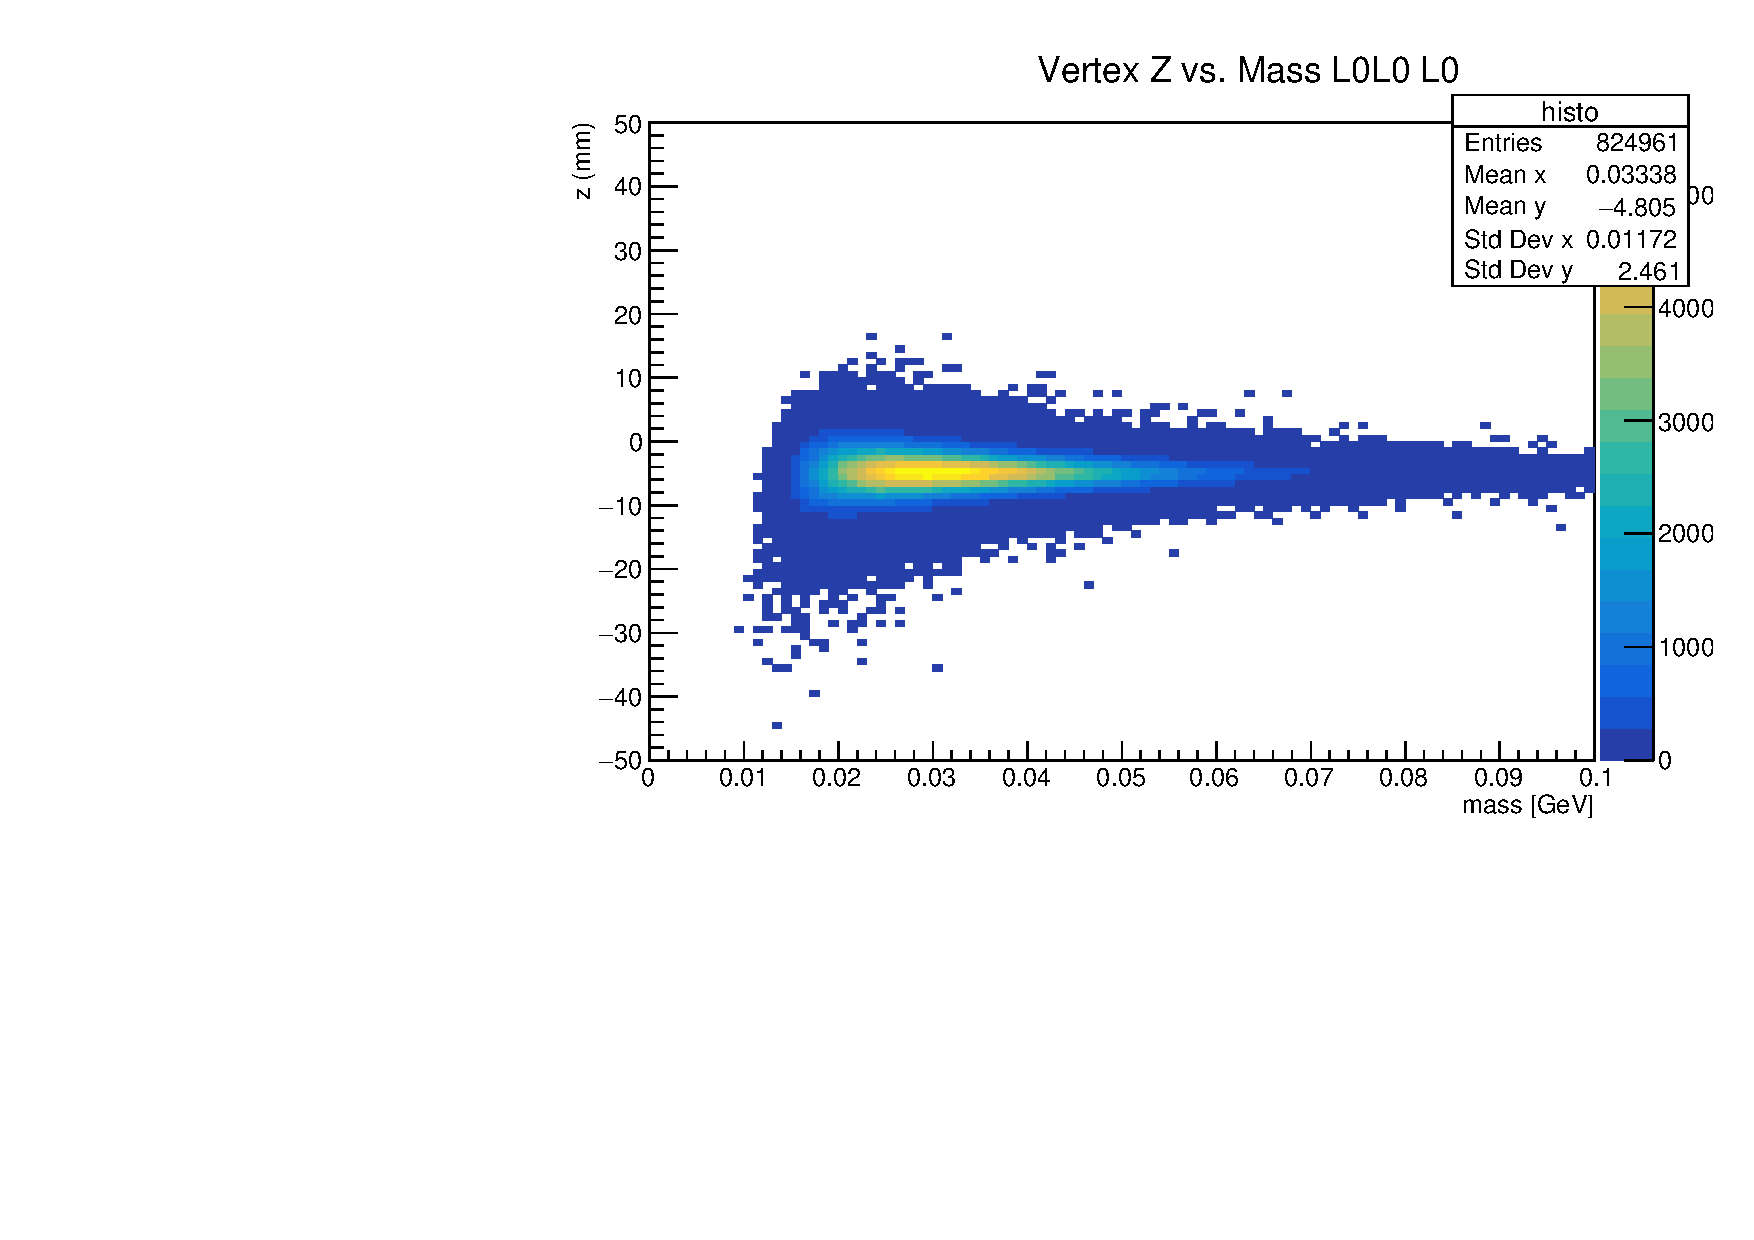
\includegraphics[width=0.3\linewidth]{figs/L0L0_loose.pdf}
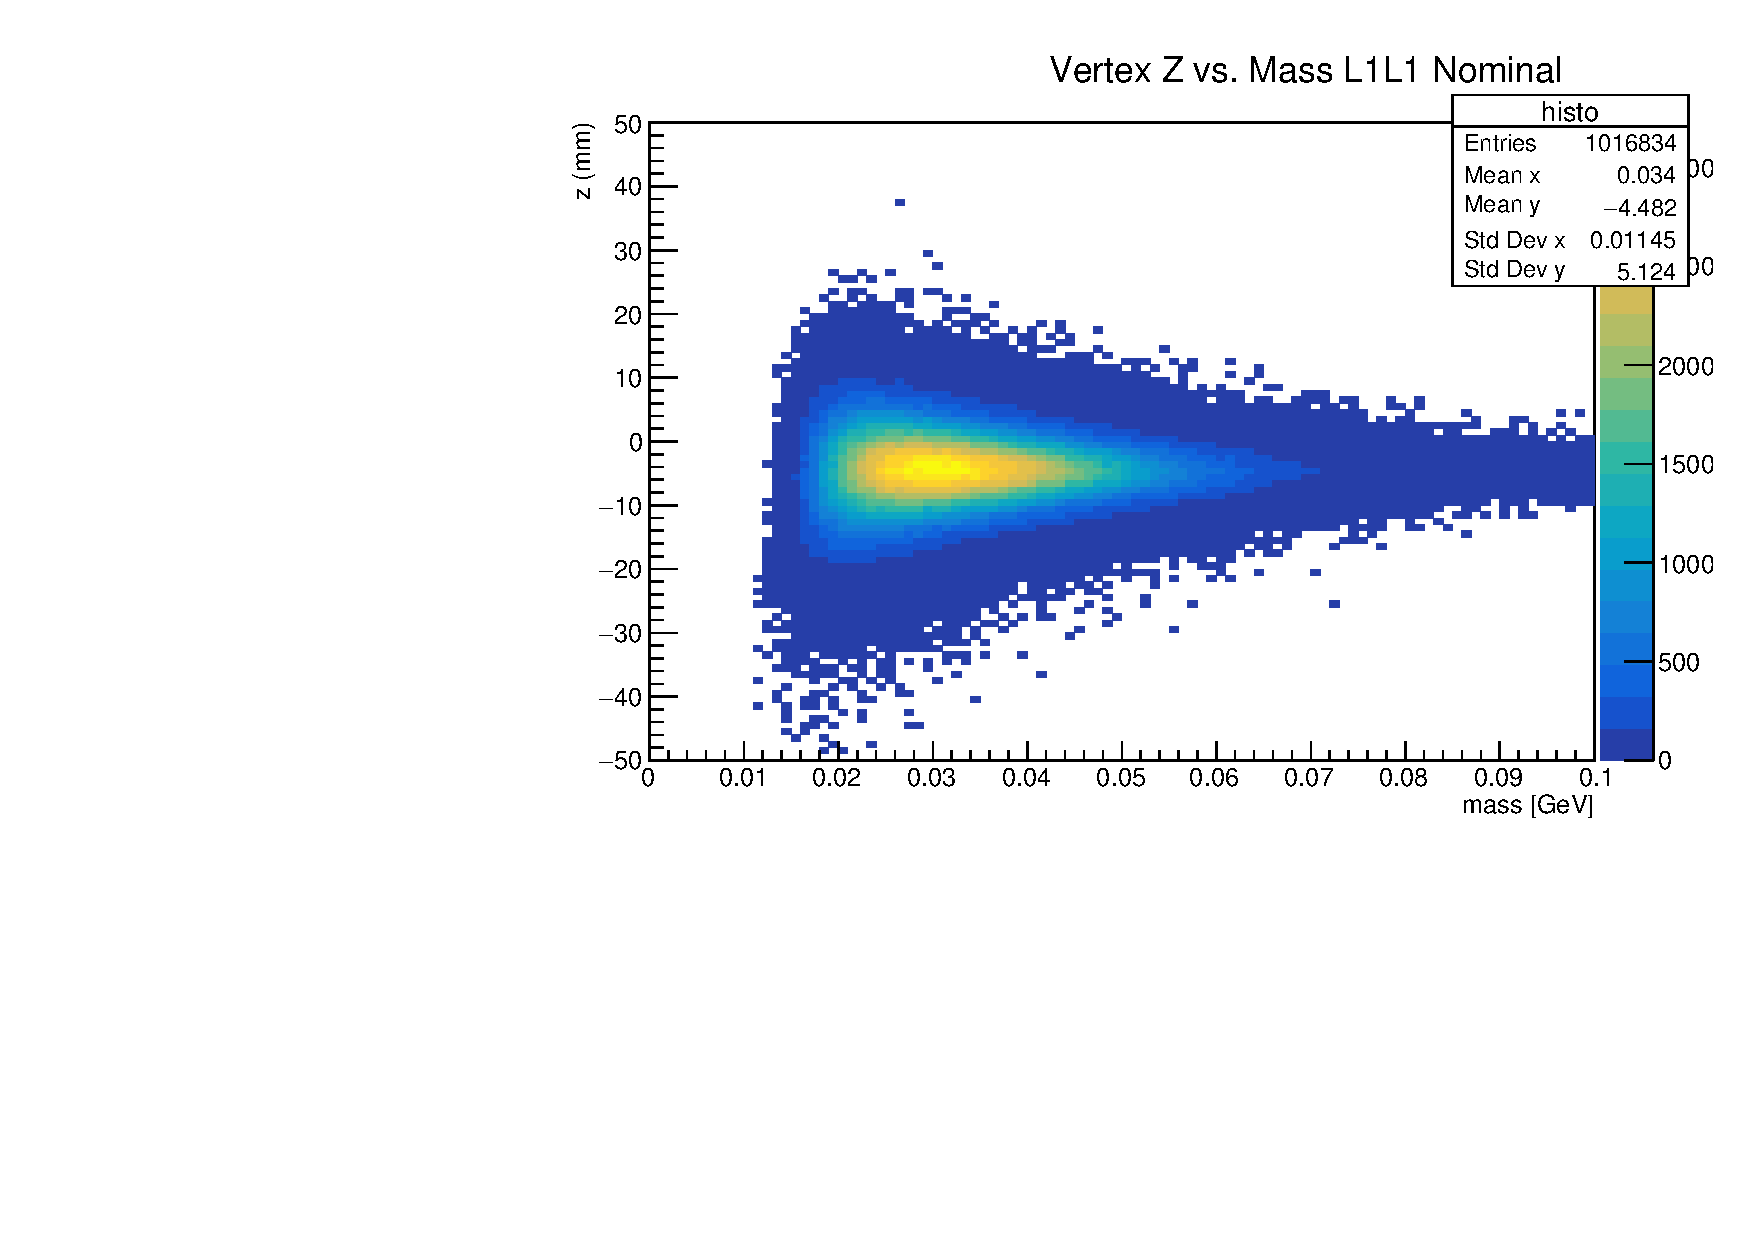
\includegraphics[width=0.3\linewidth]{figs/L1L1_loose_nom.pdf}
\end{figure}

\end{frame}

%------------------------------------------------

\begin{frame}
\frametitle{Reach Plot L0L0/L1L1 Comparison}
\begin{itemize}
\item The procedure of requiring hits in the first layer is well understood (thanks to Sho and Holly)
\item Reach plots compare L0L0 in ugrade detector vs L1L1 in the nominal detector (for a direct comparison we need L0L0 + L0L1 + L1L1 for upgrade detector, so we are underestimating our reach)
\end{itemize}
\begin{figure}
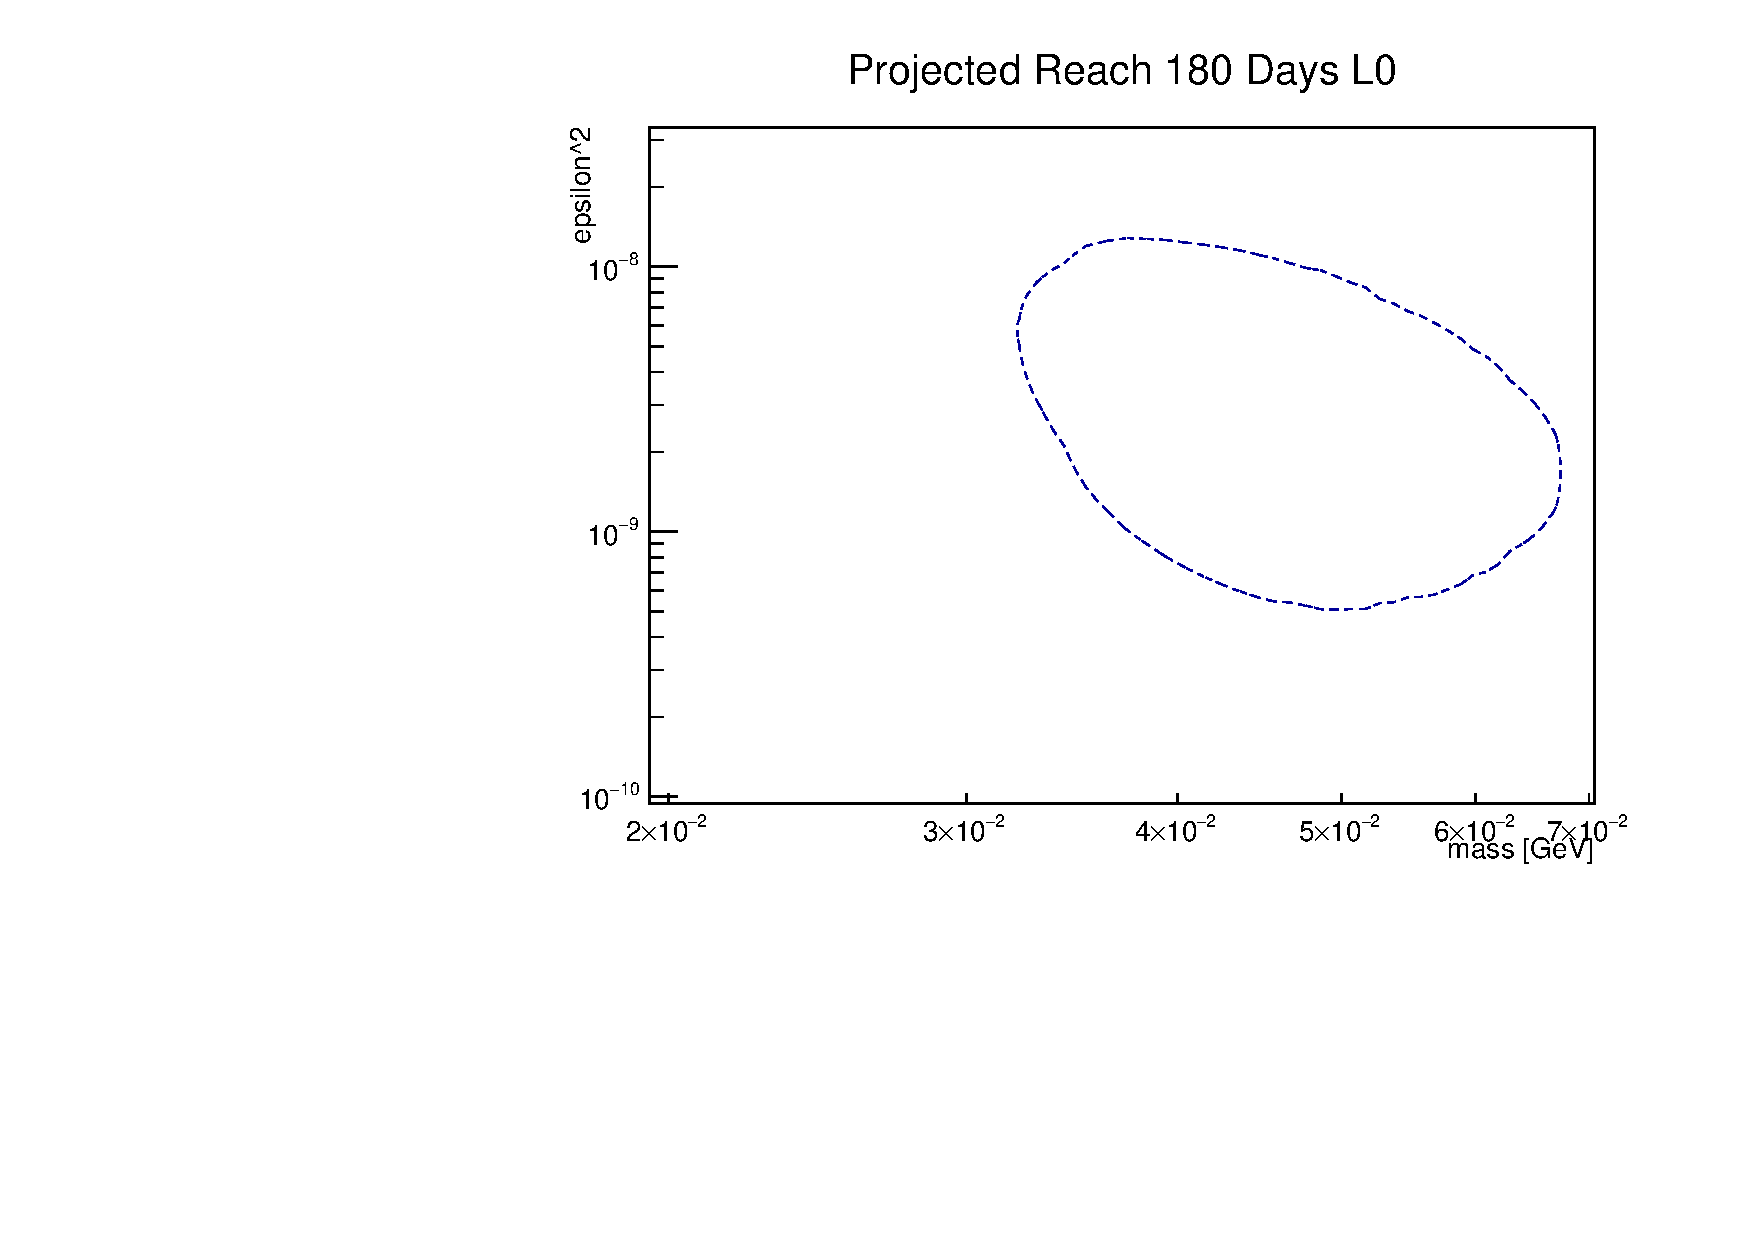
\includegraphics[width=0.4\linewidth]{figs/L0_180_days_loose.pdf}
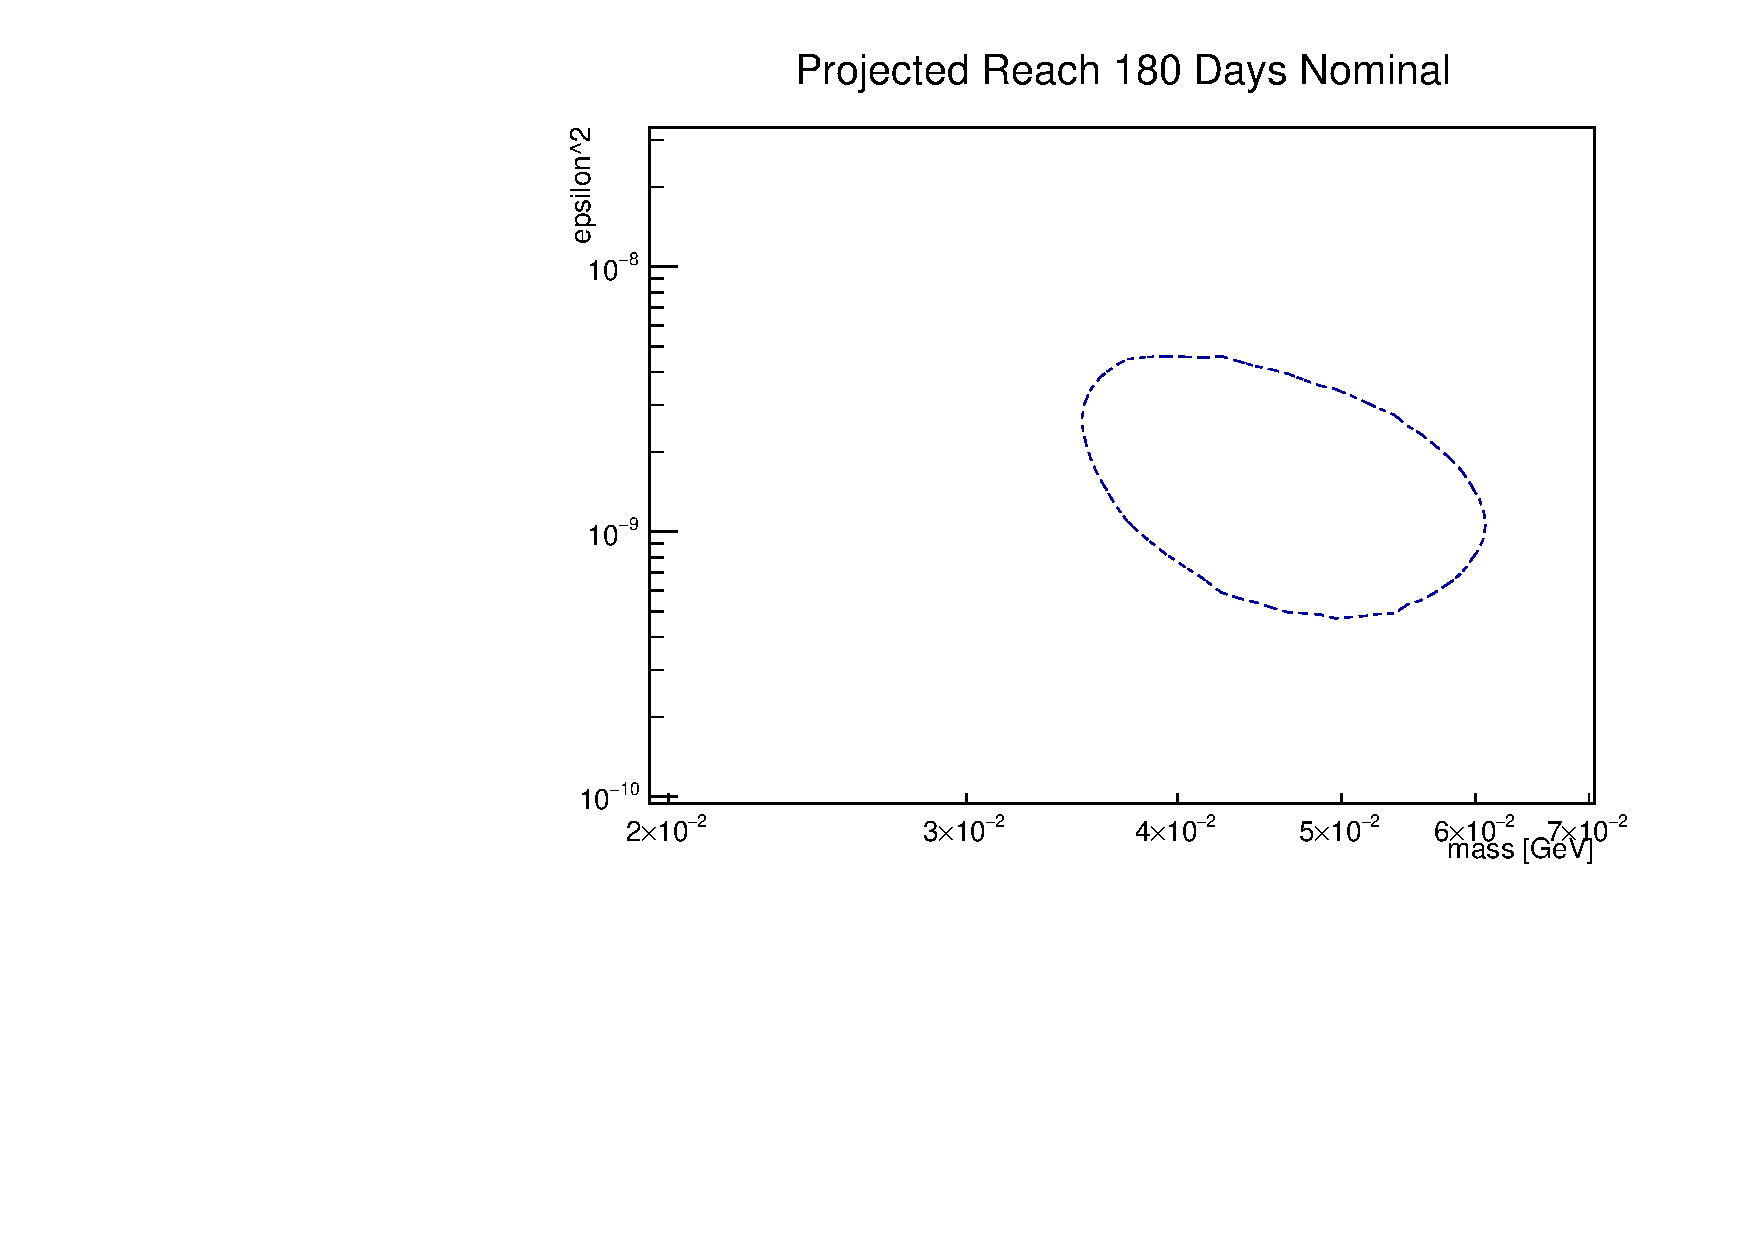
\includegraphics[width=0.4\linewidth]{figs/nom_180_days_loose.pdf}
\end{figure}

\end{frame}

%------------------------------------------------

\begin{frame}
\frametitle{Reach Plot L0L0/L1L1 Comparison (cont.)}
\begin{figure}
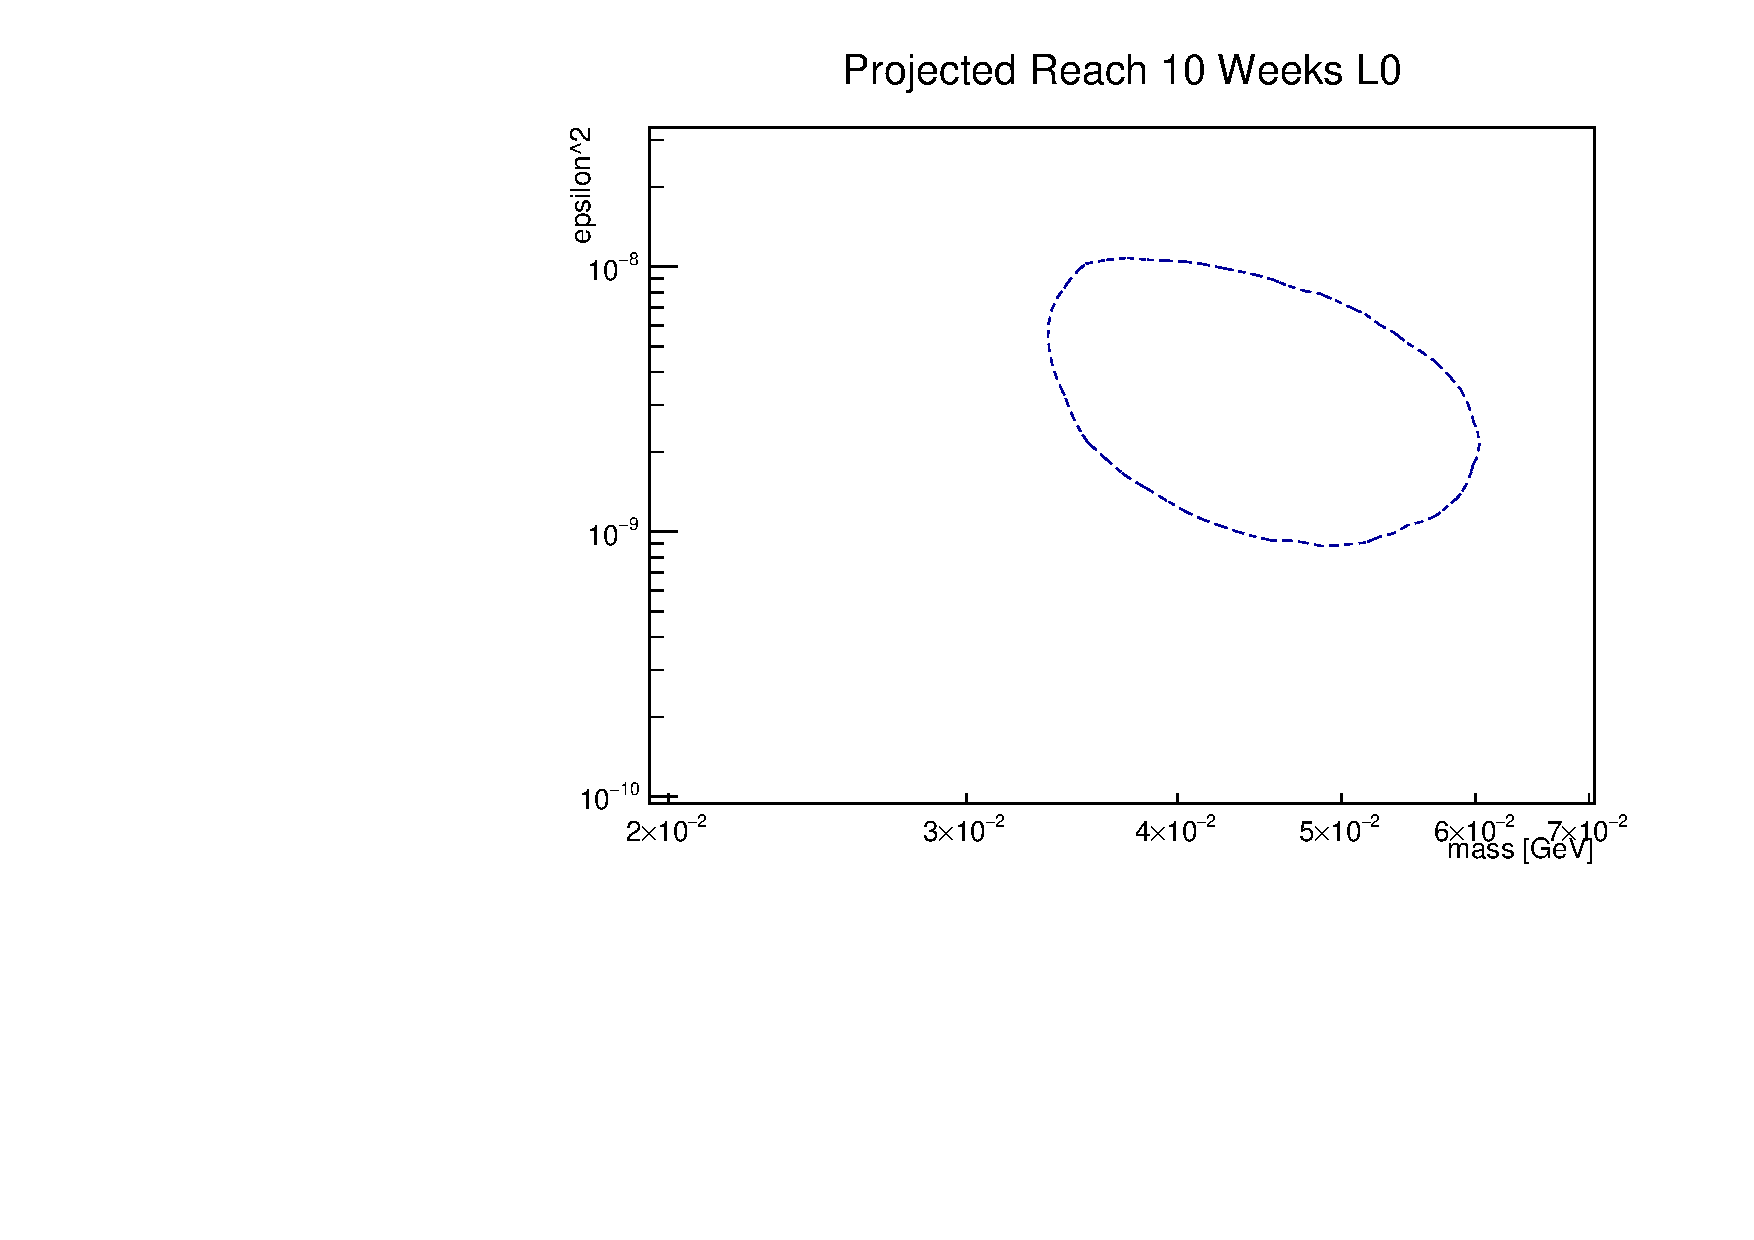
\includegraphics[width=0.4\linewidth]{figs/L0_10_weeks_loose.pdf}
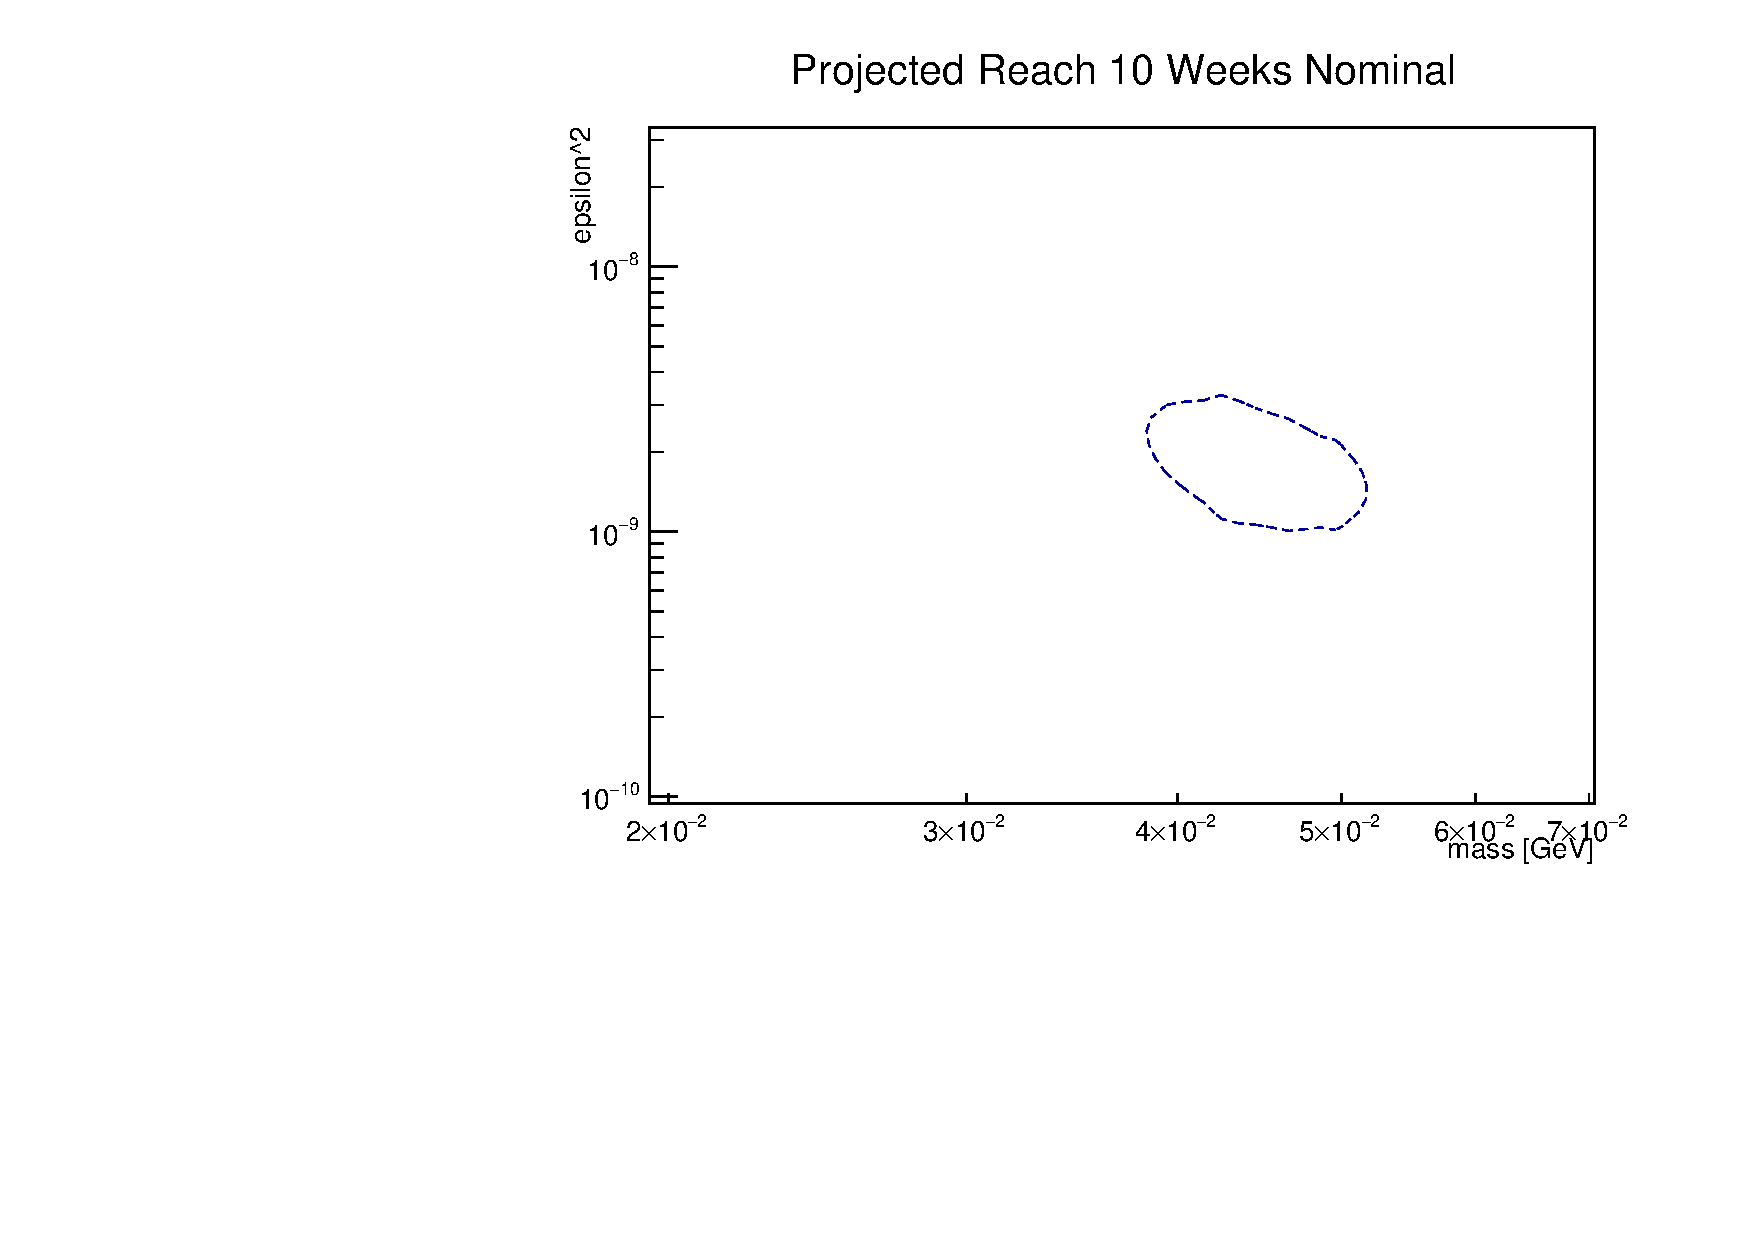
\includegraphics[width=0.4\linewidth]{figs/nom_10_weeks_loose.pdf}
\end{figure}
\begin{figure}
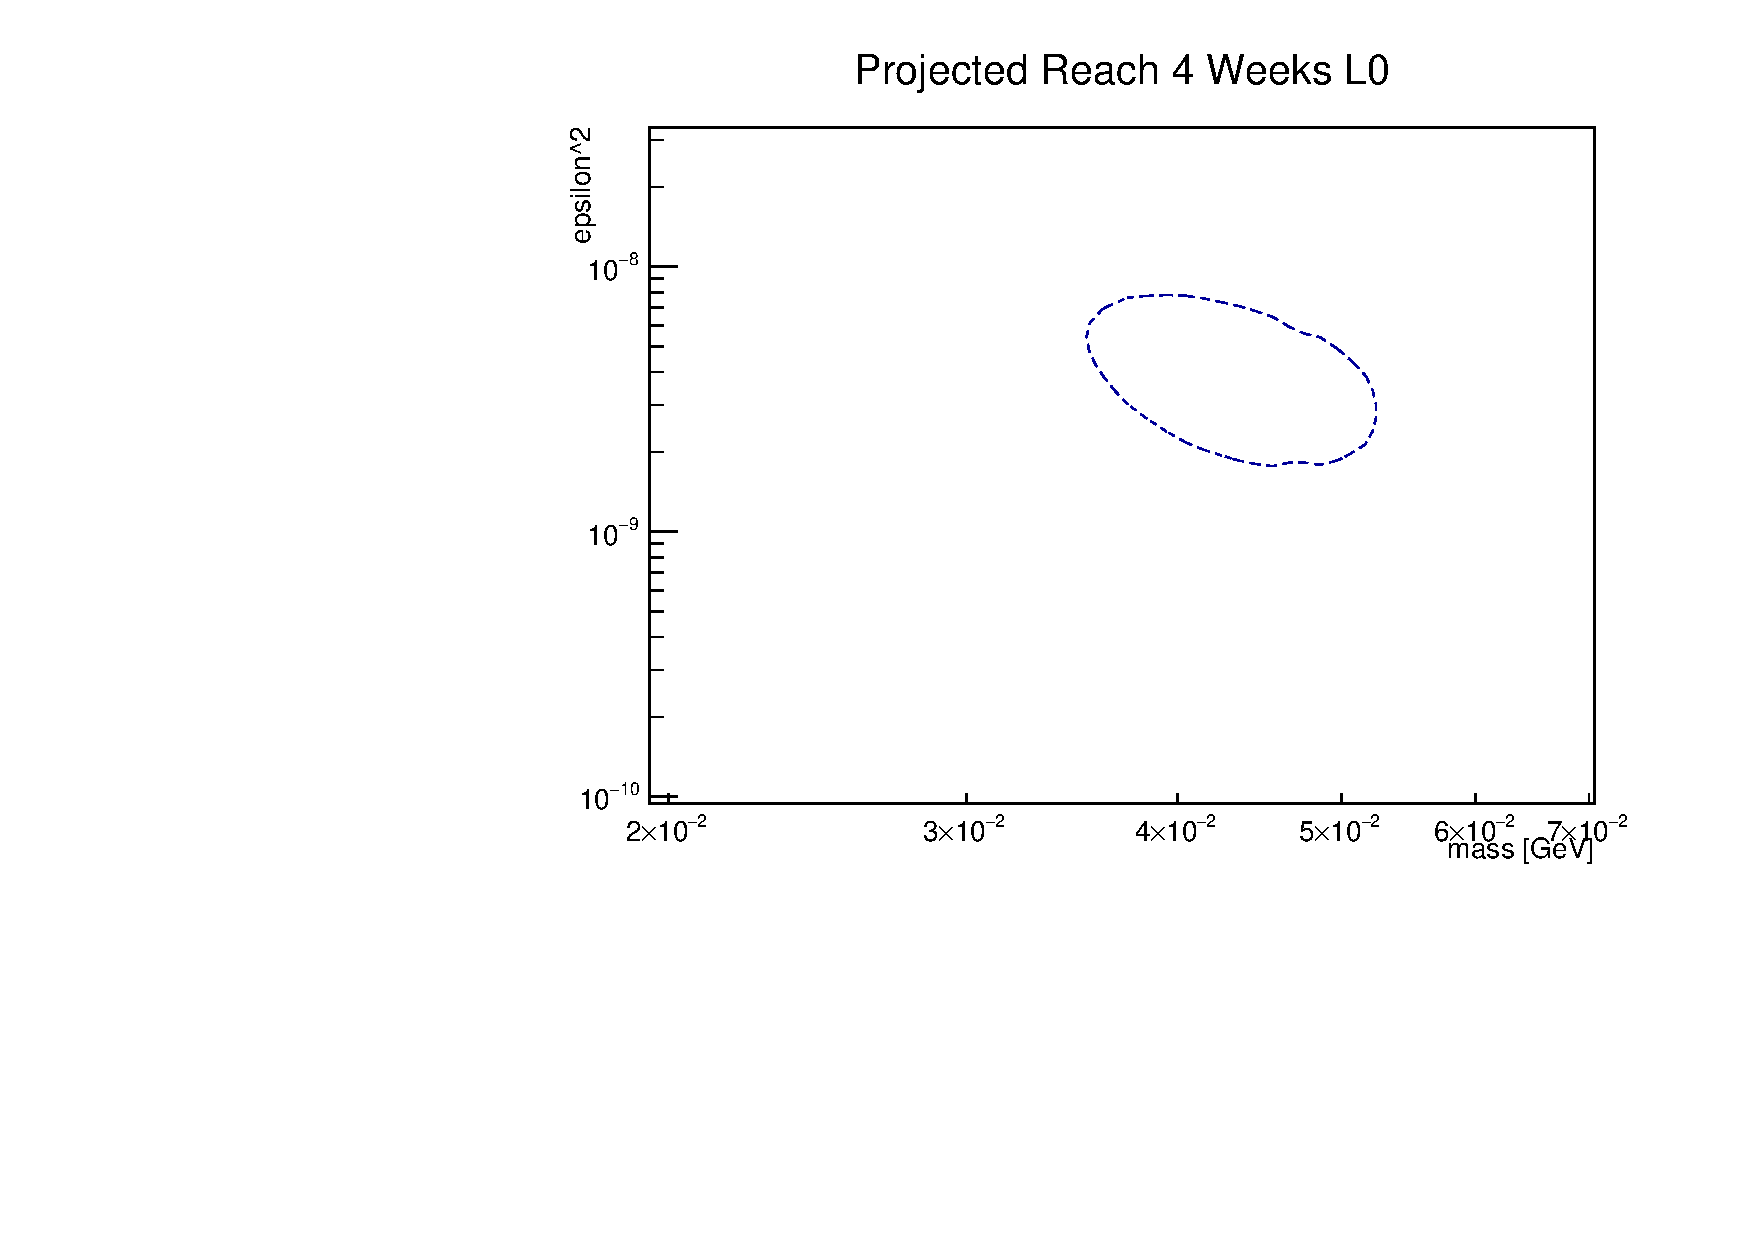
\includegraphics[width=0.4\linewidth]{figs/L0_4_weeks_loose.pdf}
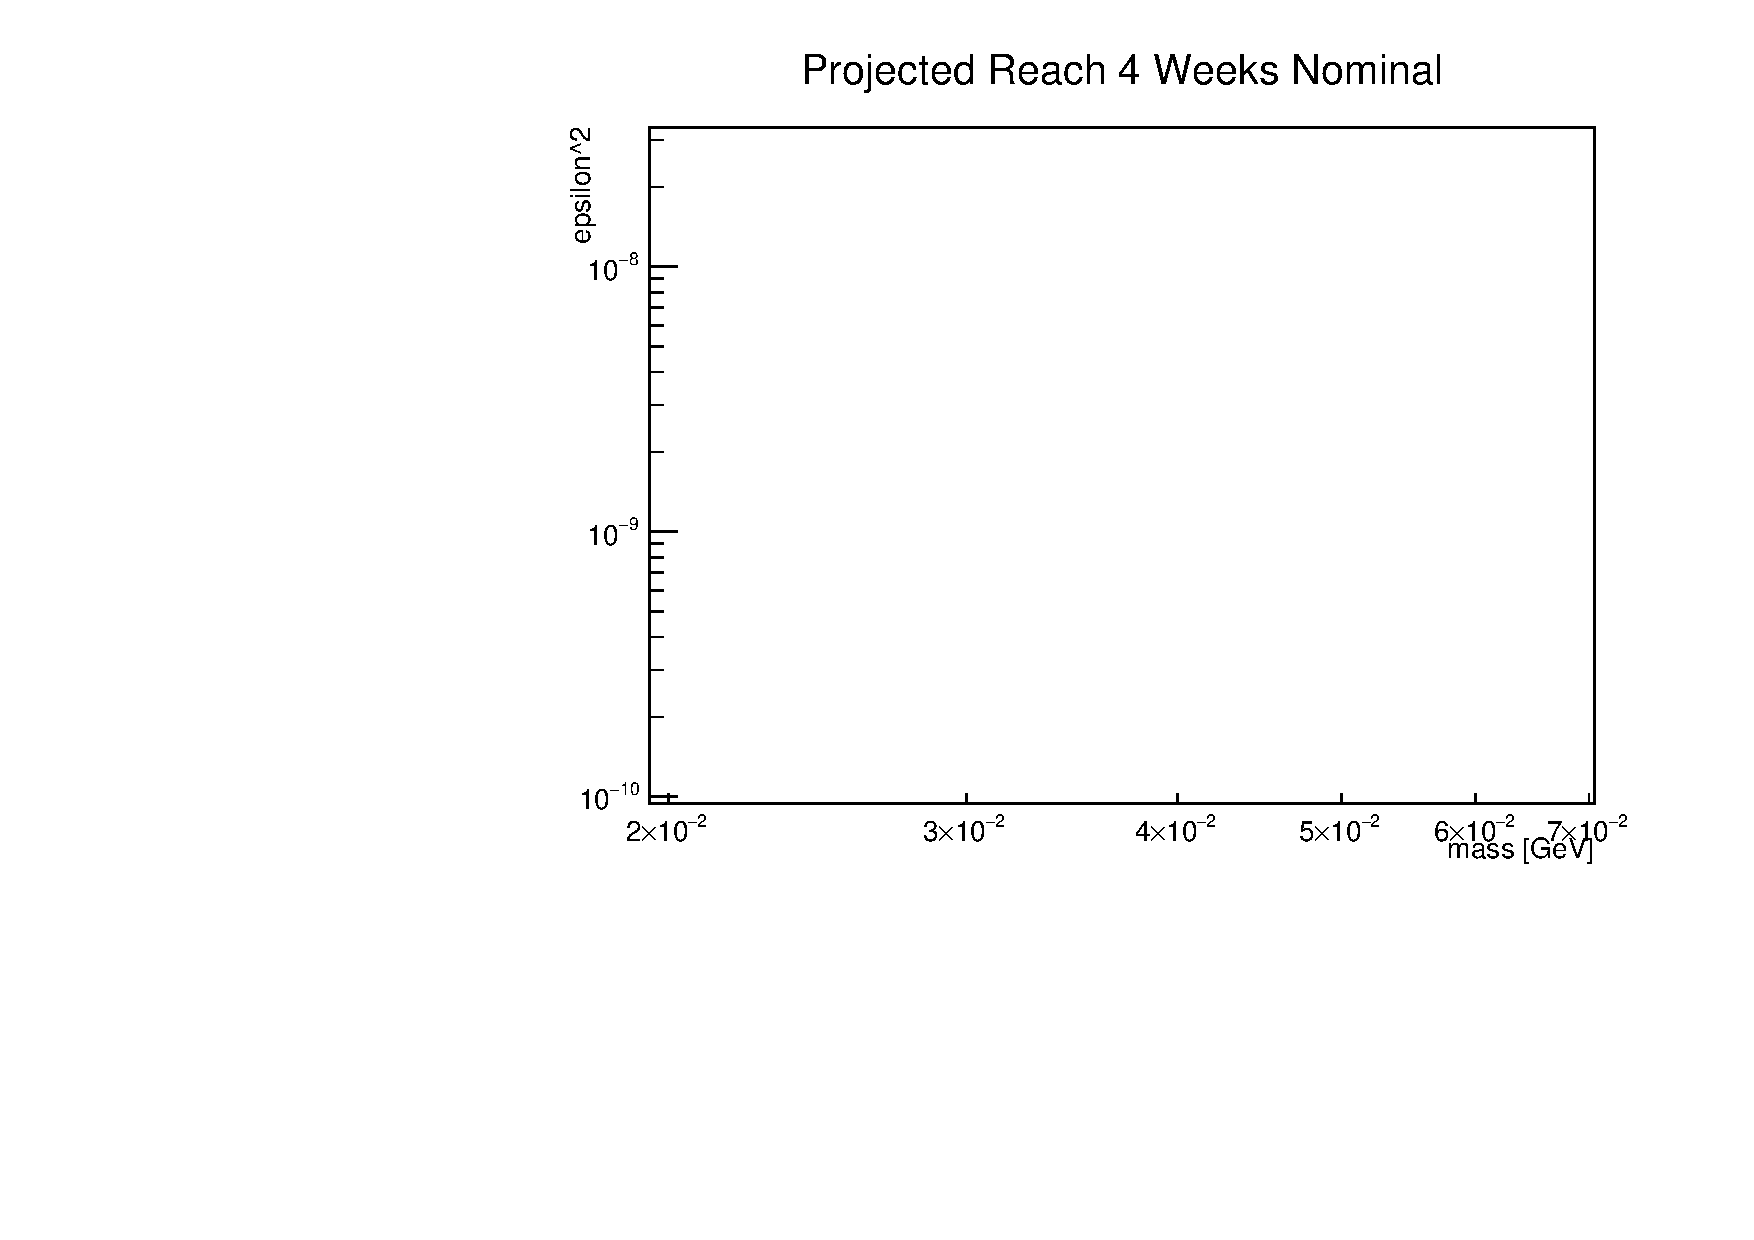
\includegraphics[width=0.4\linewidth]{figs/nom_4_weeks_loose.pdf}
\end{figure}

\end{frame}

%------------------------------------------------

\begin{frame}
\frametitle{Number A's Detectable L0L0/L1L1}
\begin{itemize}
\item Number of detectable A's past all cuts comparing L0L0 for L0 and L1L1 for nominal at 180 days
\end{itemize}
\begin{figure}
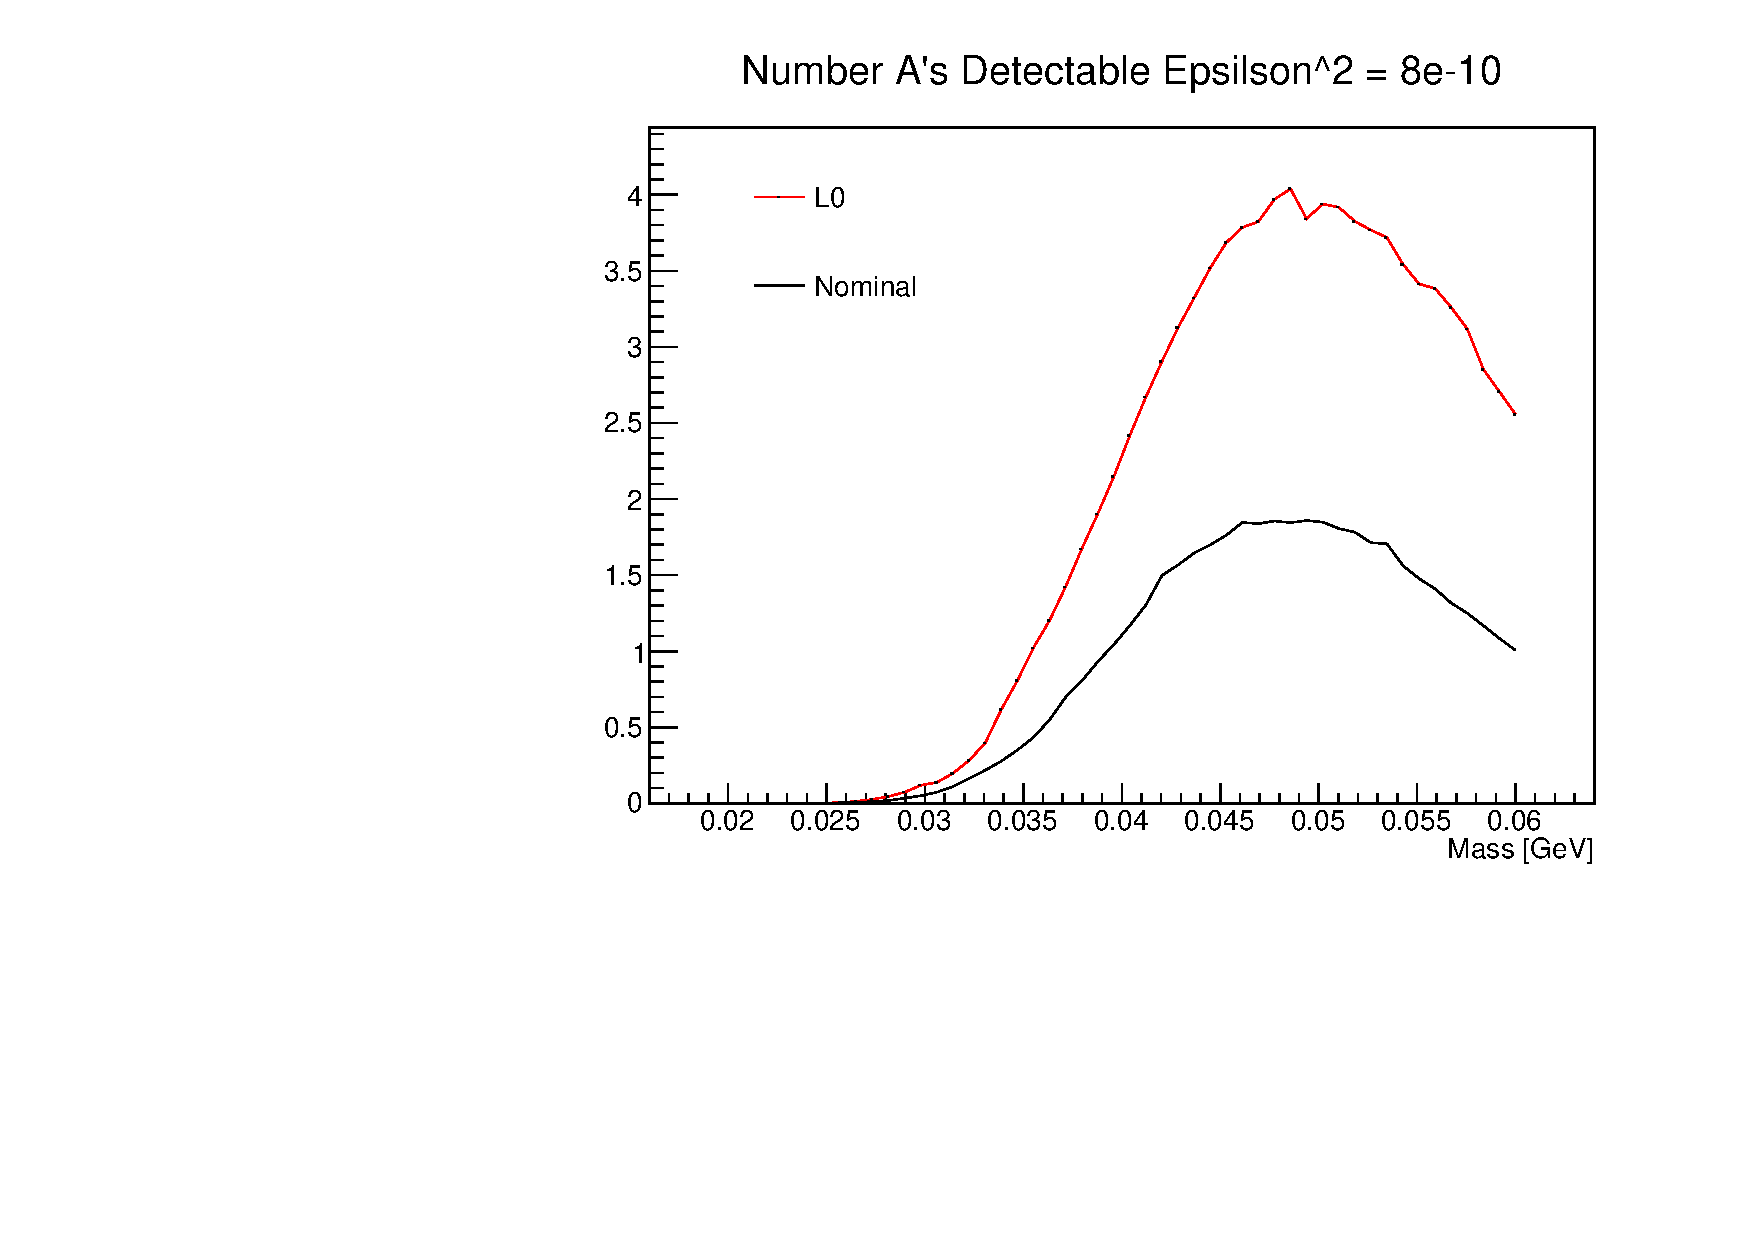
\includegraphics[width=0.36\linewidth]{figs/detectable_8e-10.pdf}
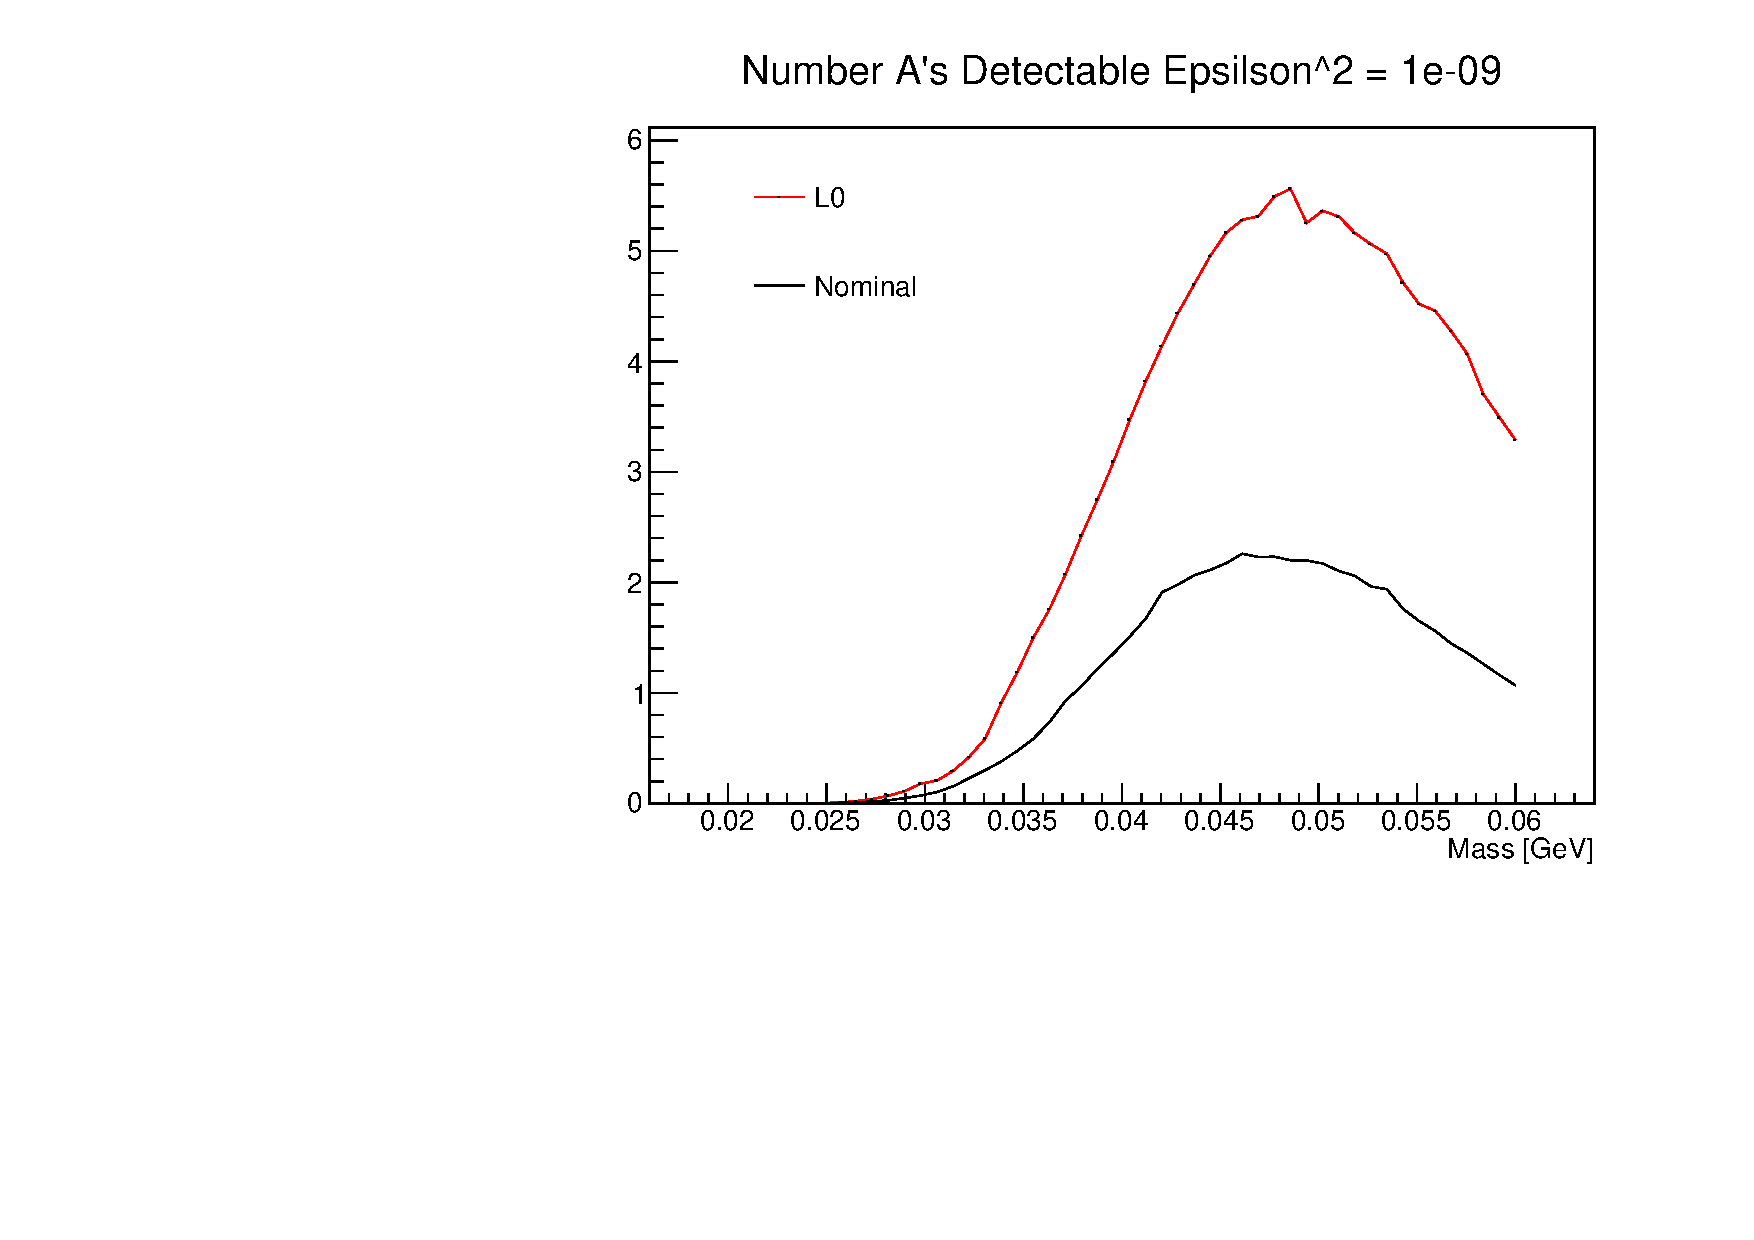
\includegraphics[width=0.36\linewidth]{figs/detectable_1e-09.pdf}
\end{figure}
\begin{figure}
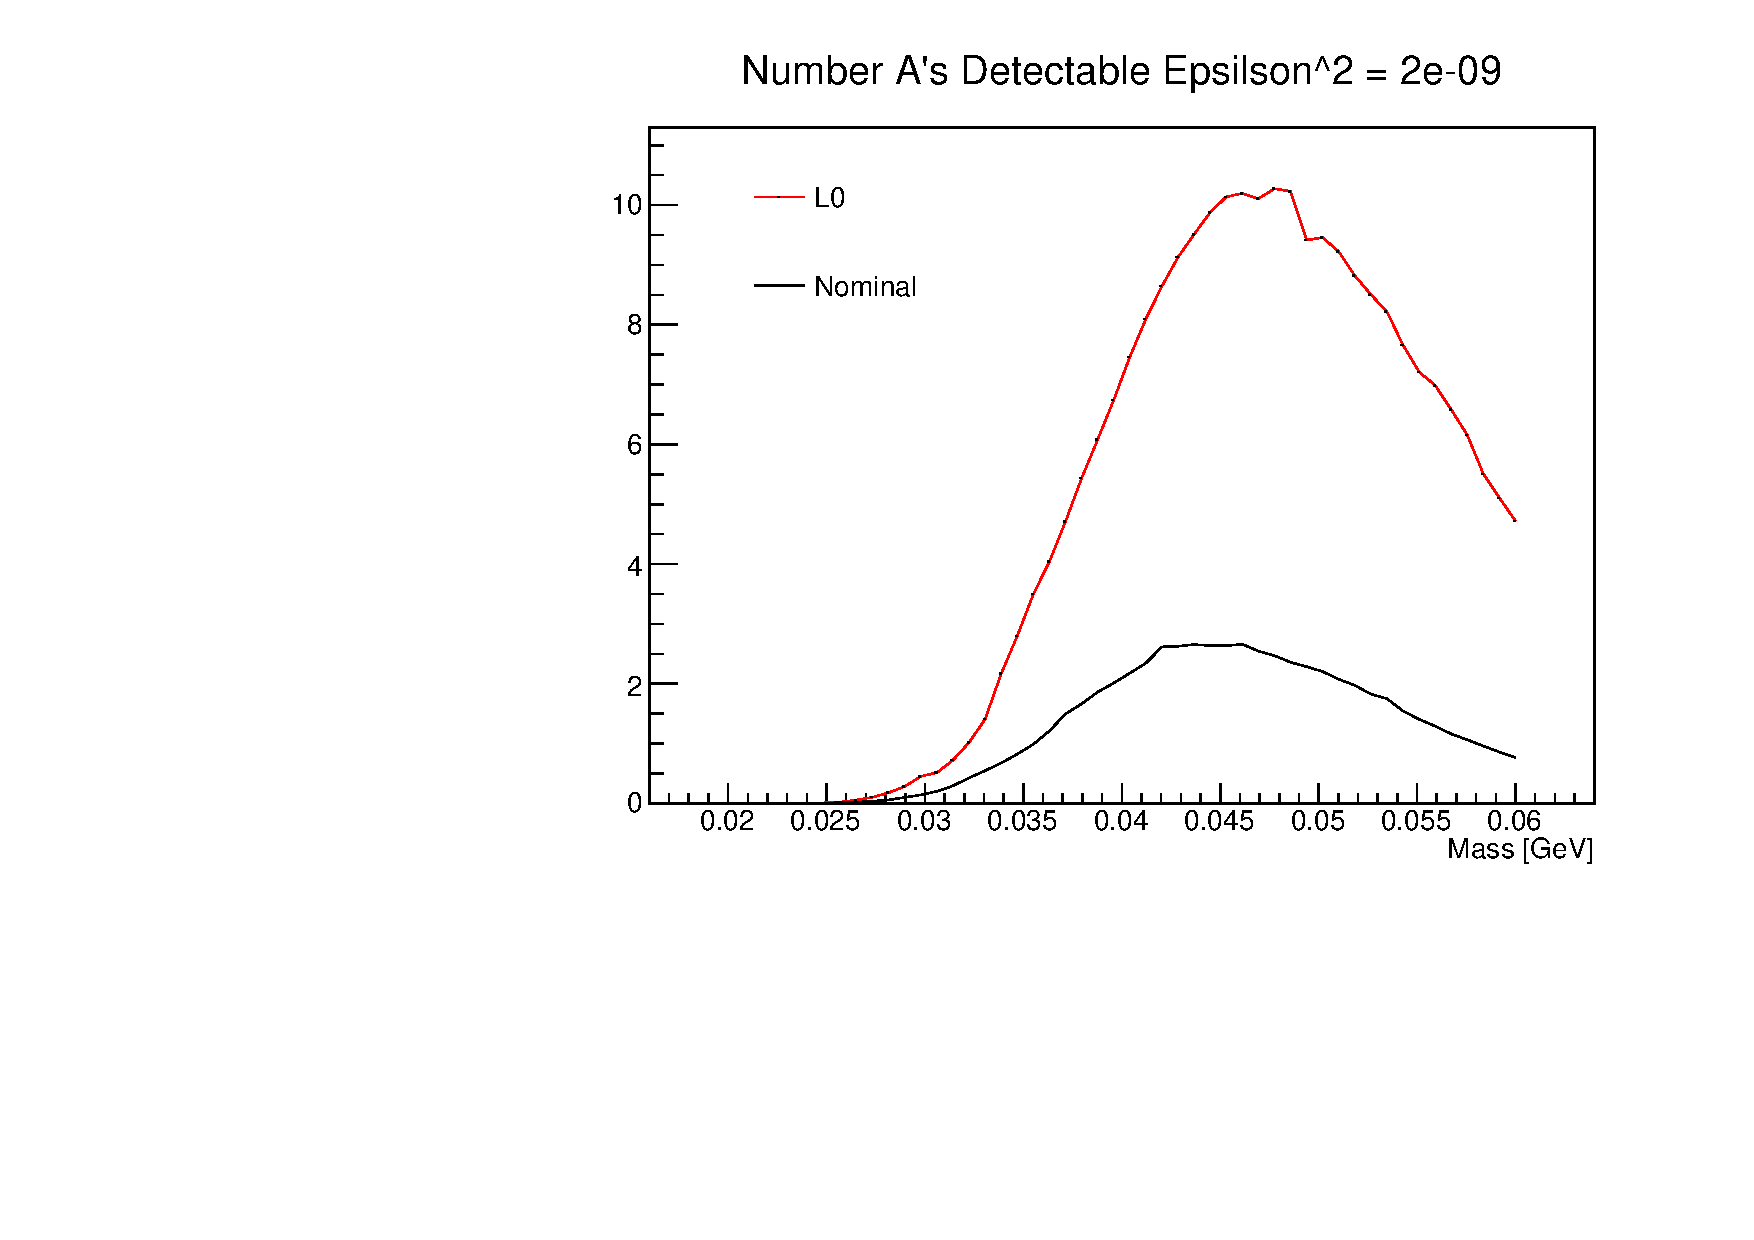
\includegraphics[width=0.36\linewidth]{figs/detectable_2e-09.pdf}
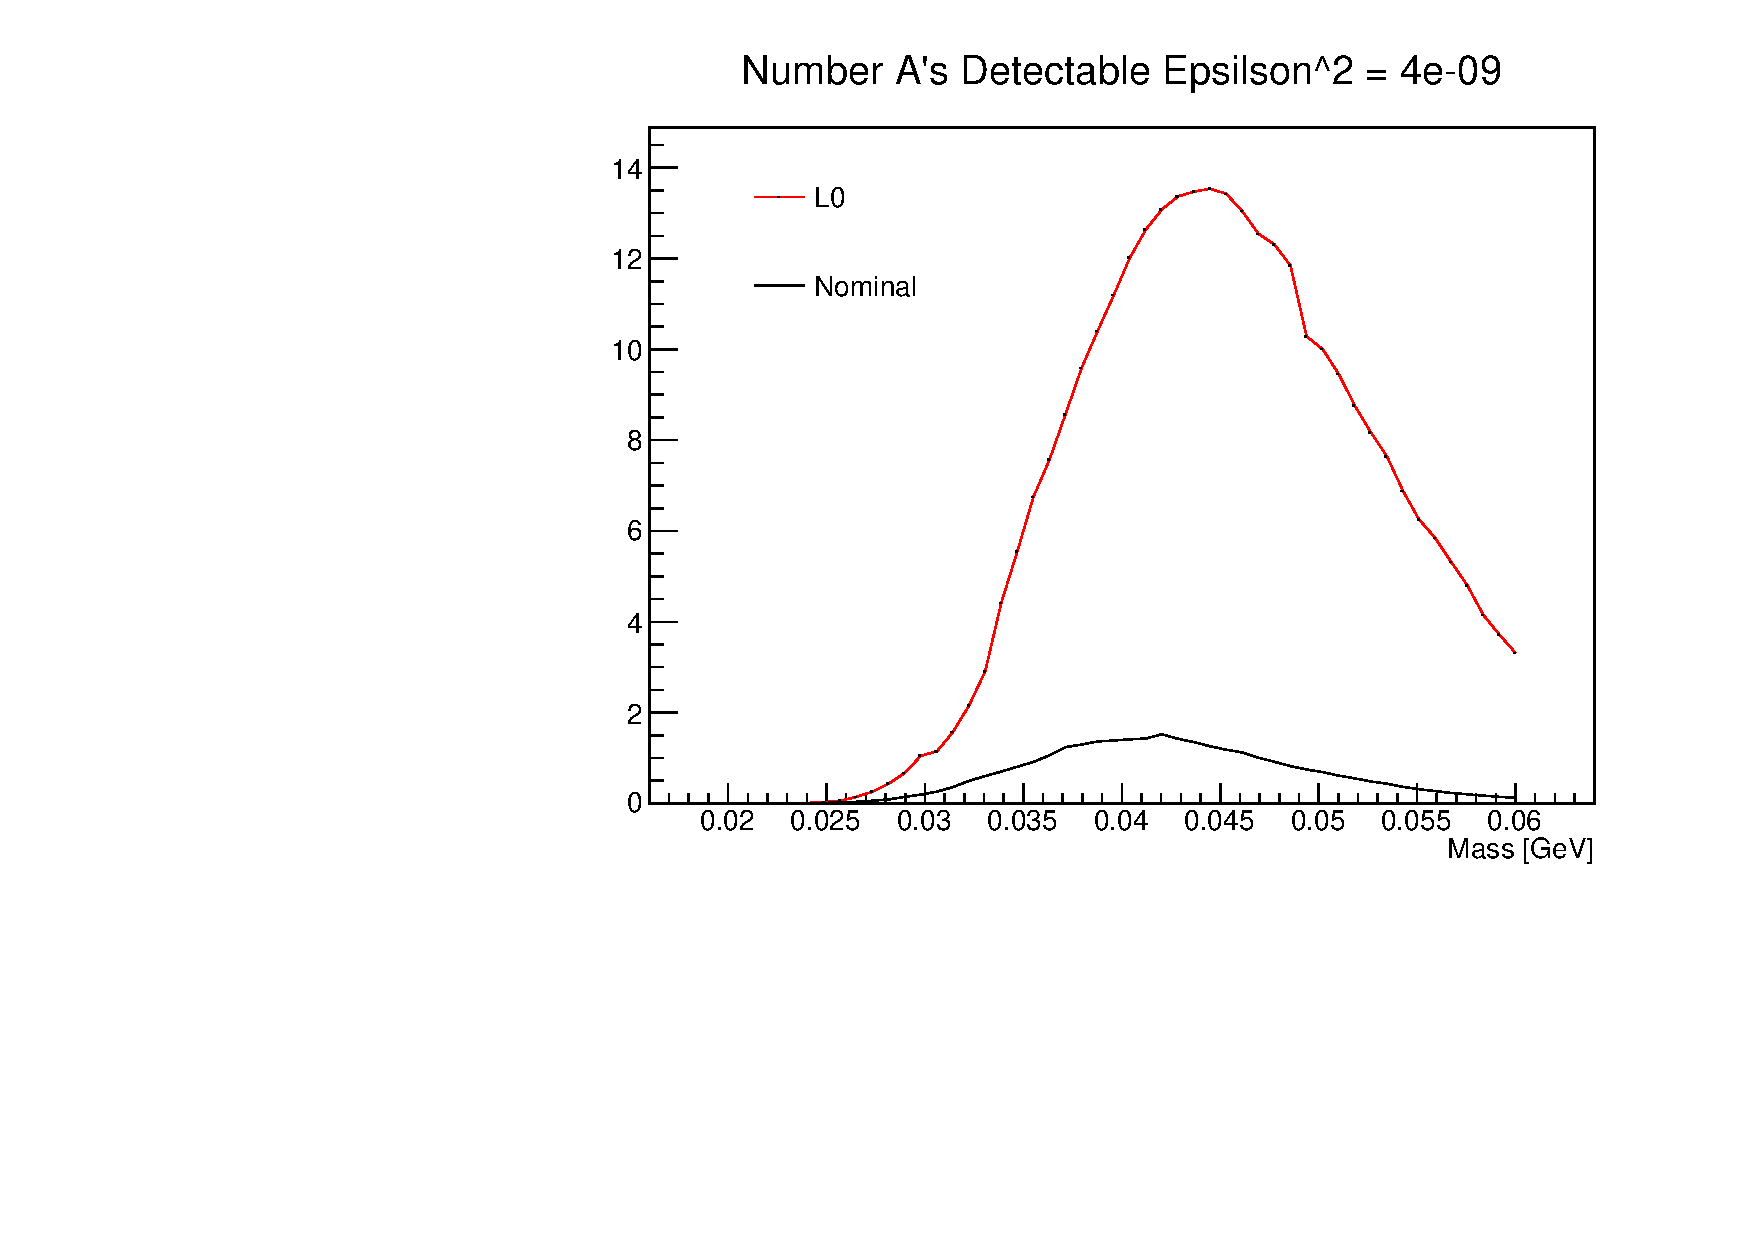
\includegraphics[width=0.36\linewidth]{figs/detectable_4e-09.pdf}
\end{figure}

\end{frame}

%------------------------------------------------

\begin{frame}
\frametitle{Difficulty With Other Layer Requirements}
\begin{itemize}
\item Backgrounds due to hit \textcolor{darkgray}{\textbf{inefficiencies are cut out by extrapolating track to active sensor}} (inefficiencies are NOT present in MC)
\item Remaining background is due to a \textcolor{darkgray}{\textbf{hard scatter in the dead silicon}} into the acceptance of the rest of the tracker% (either trident/beam particle, or converted wab with hard scatter)
\end{itemize}
\begin{figure}
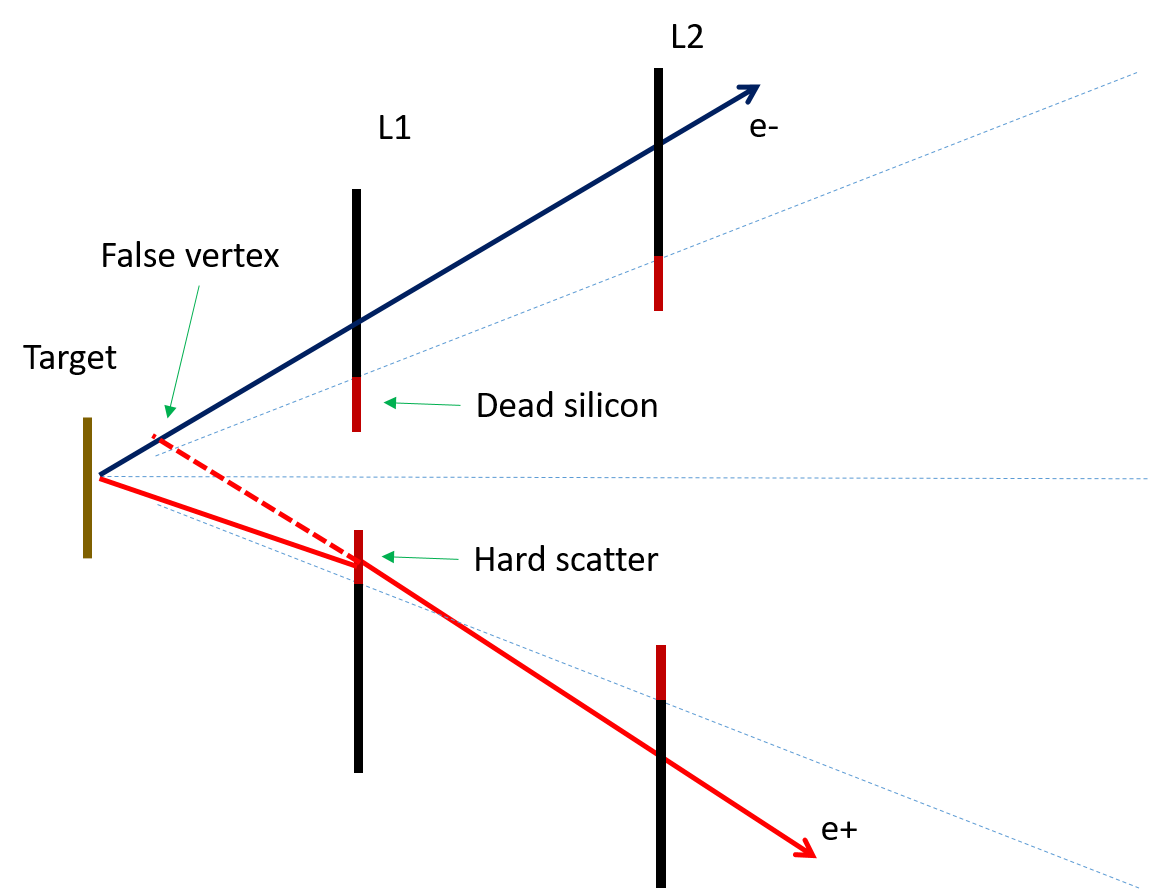
\includegraphics[width=0.55\linewidth]{figs/Scattering_schematic.png}
\end{figure}

\end{frame}

%------------------------------------------------

\begin{frame}
\frametitle{Difficulty With Other Layer Requirements (cont.)}
\begin{itemize}
\item Shifts peak of the distribution towards larger $z$
\item Curves show the fraction of efficiency curve (i.e. the 10\% curve is the $z_{0.10}$ is the solution to $\frac{\int_{z_{targ}}^{z_{0.10}}eff(z)dz}{\int_{z_{targ}}^{z_{max}}eff(z)dz}=0.10$)
\item Higher mass has larger $z$ efficiency curves (may not even need zcut)
\end{itemize}
\begin{figure}
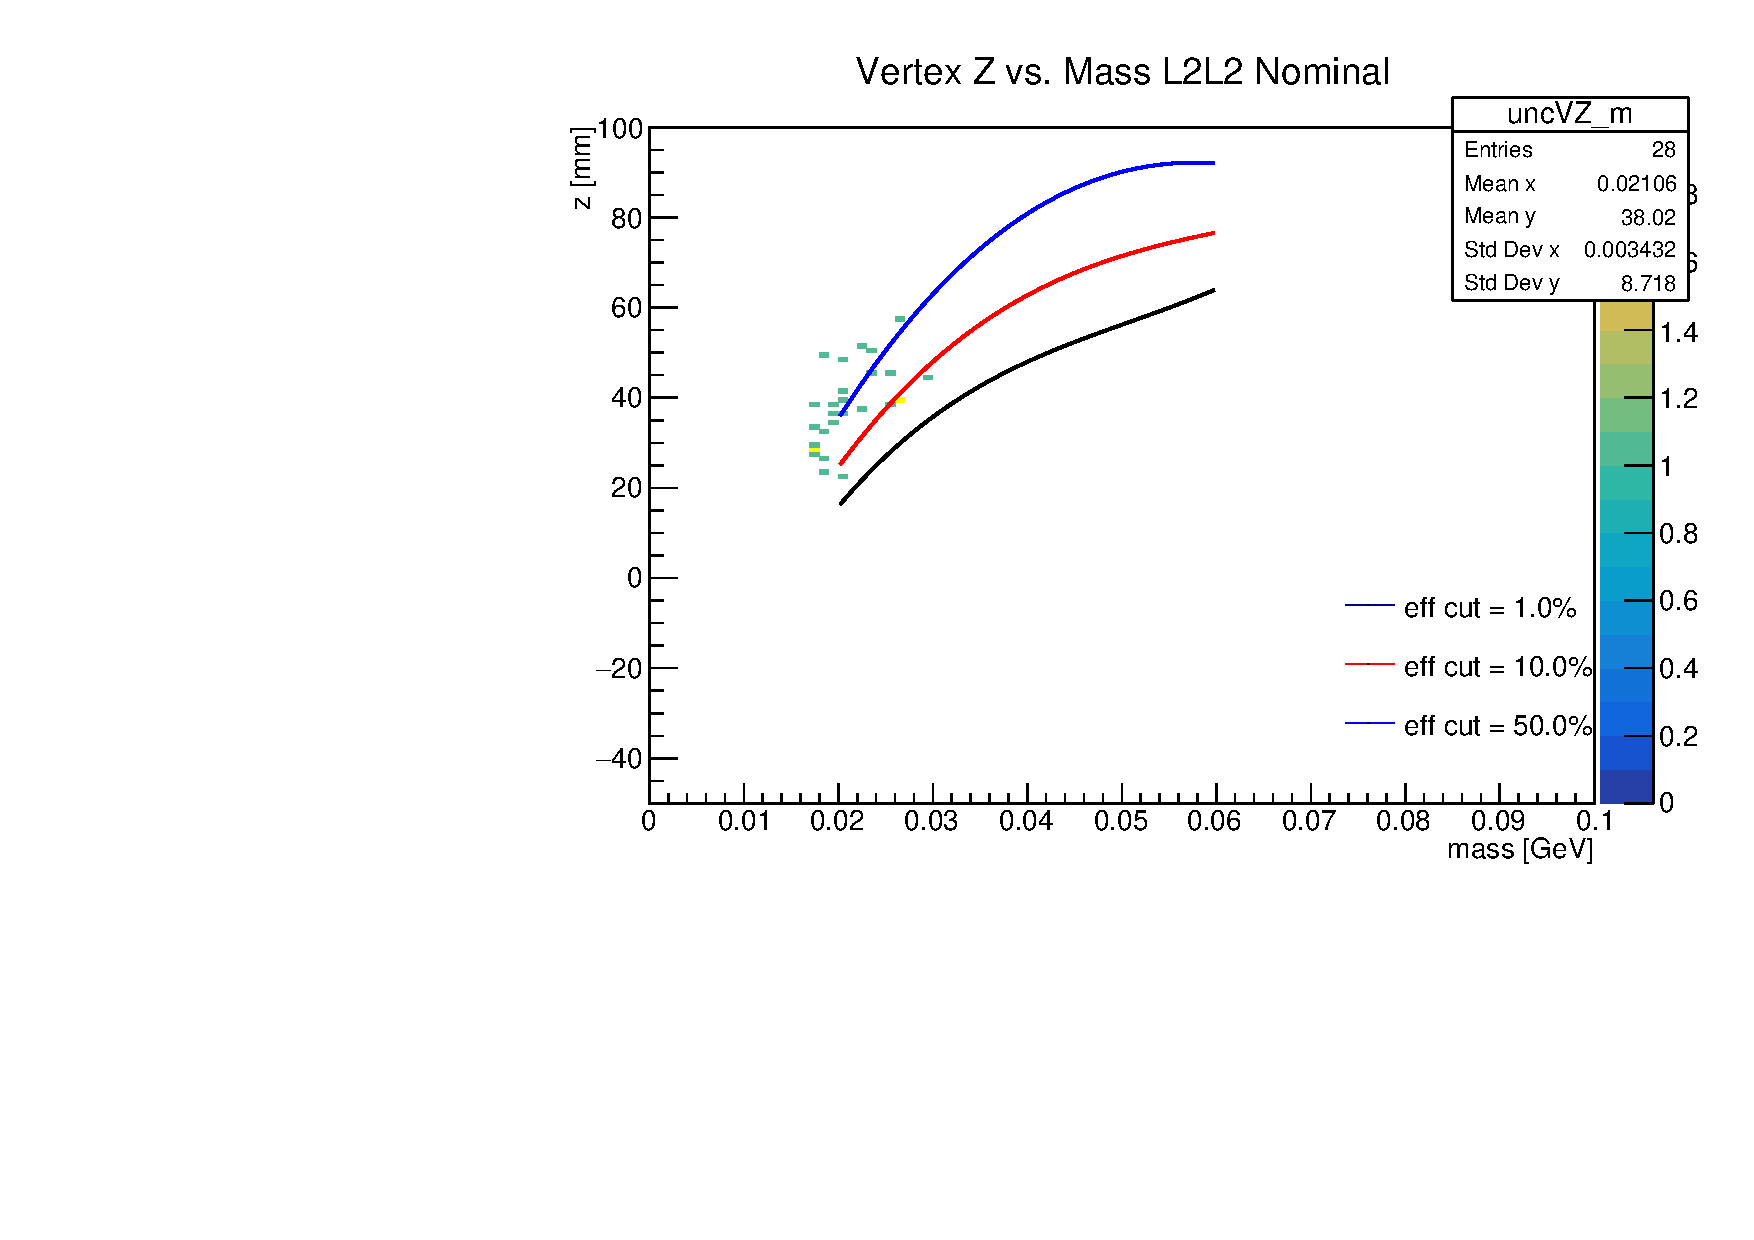
\includegraphics[width=0.4\linewidth]{figs/L2L2_sharedcut.pdf}
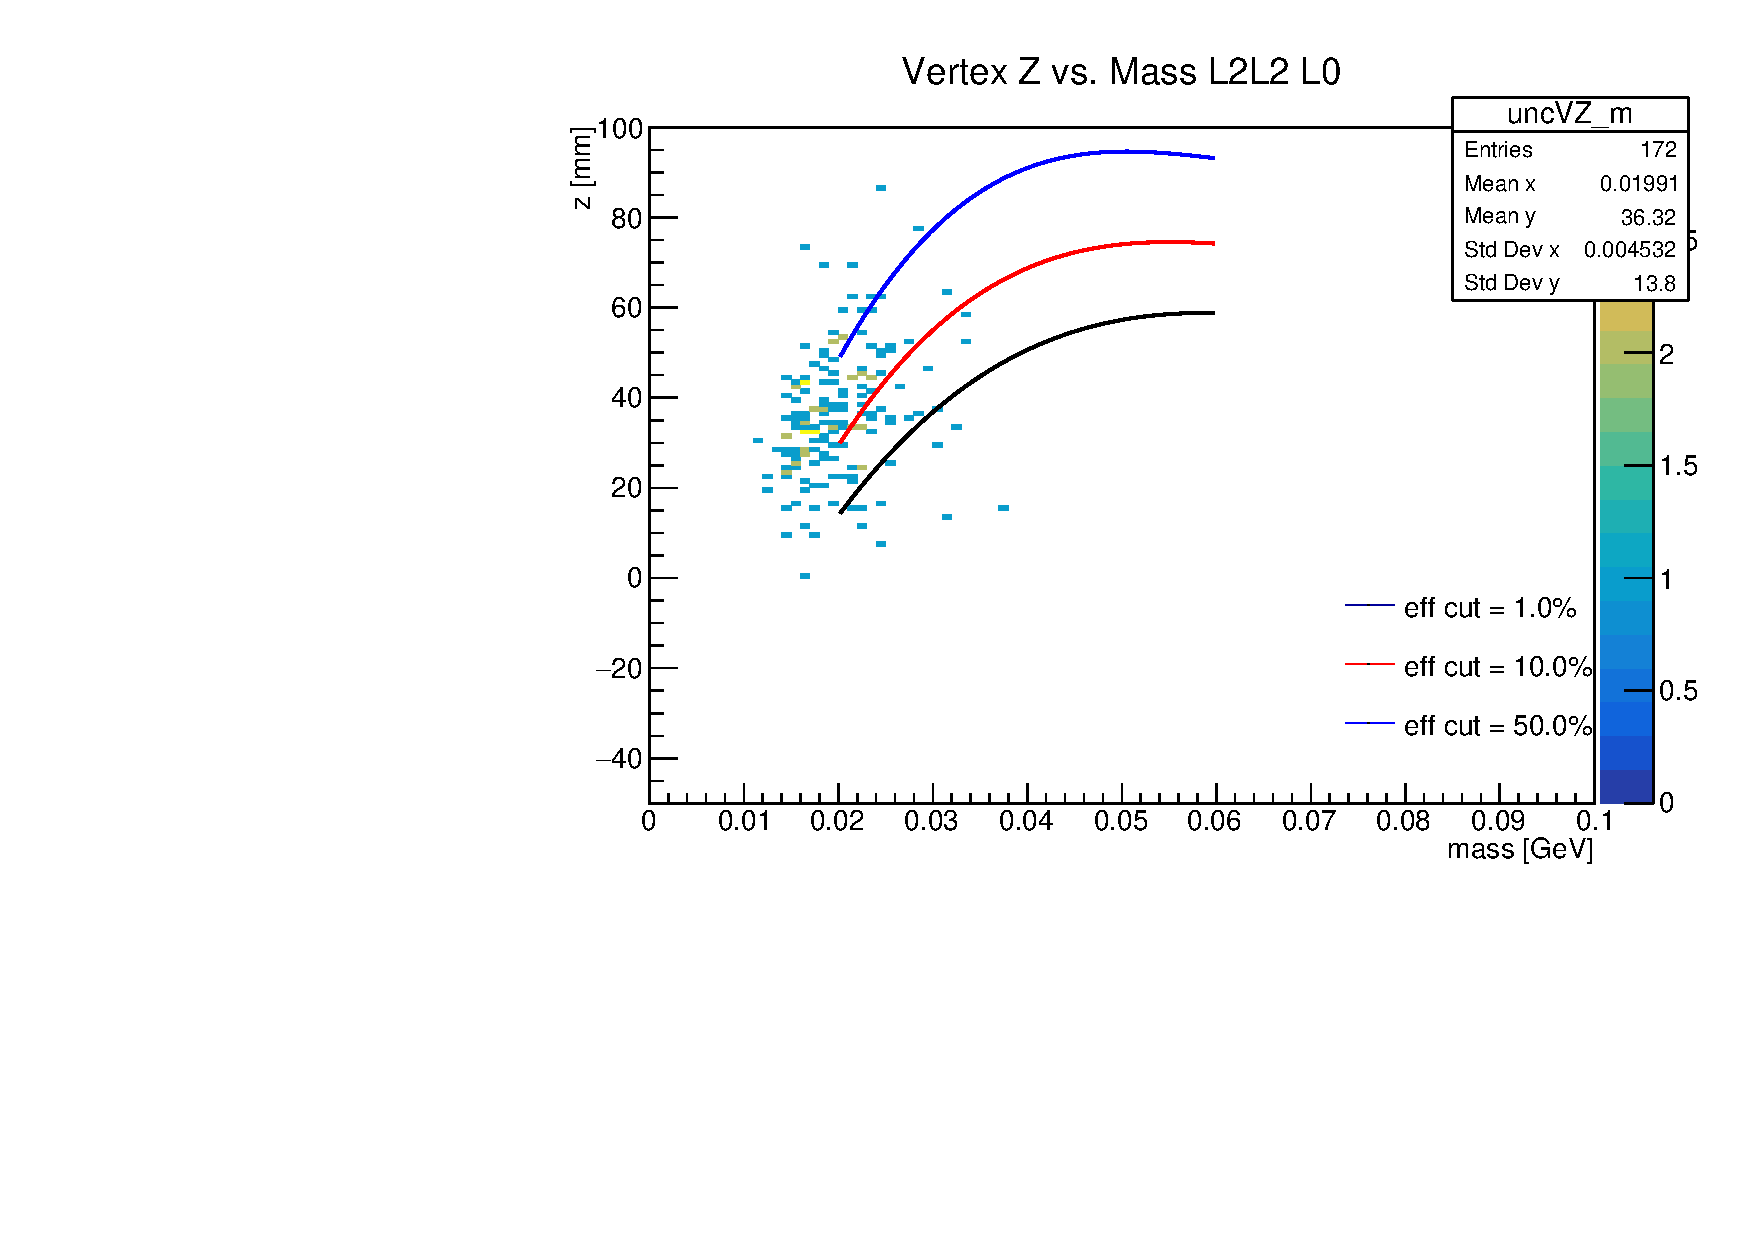
\includegraphics[width=0.4\linewidth]{figs/L2L2_loose.pdf}
\end{figure}

\end{frame}

%------------------------------------------------

\begin{frame}
\frametitle{Other Layer Requirements Vz vs. Mass Nominal}
\begin{itemize}
\item Can we trust this MC? Does this agree with data?
\item In data, L1L2 has 30,000 events and L2L2 has 250 events at 120 1/nb (compared to 155 1/nb in MC)
\item In the near future,\textcolor{darkgray}{\textbf{ add the correct proportion of wabs and tighten up track extrapolation cut}}
\end{itemize}
\begin{figure}
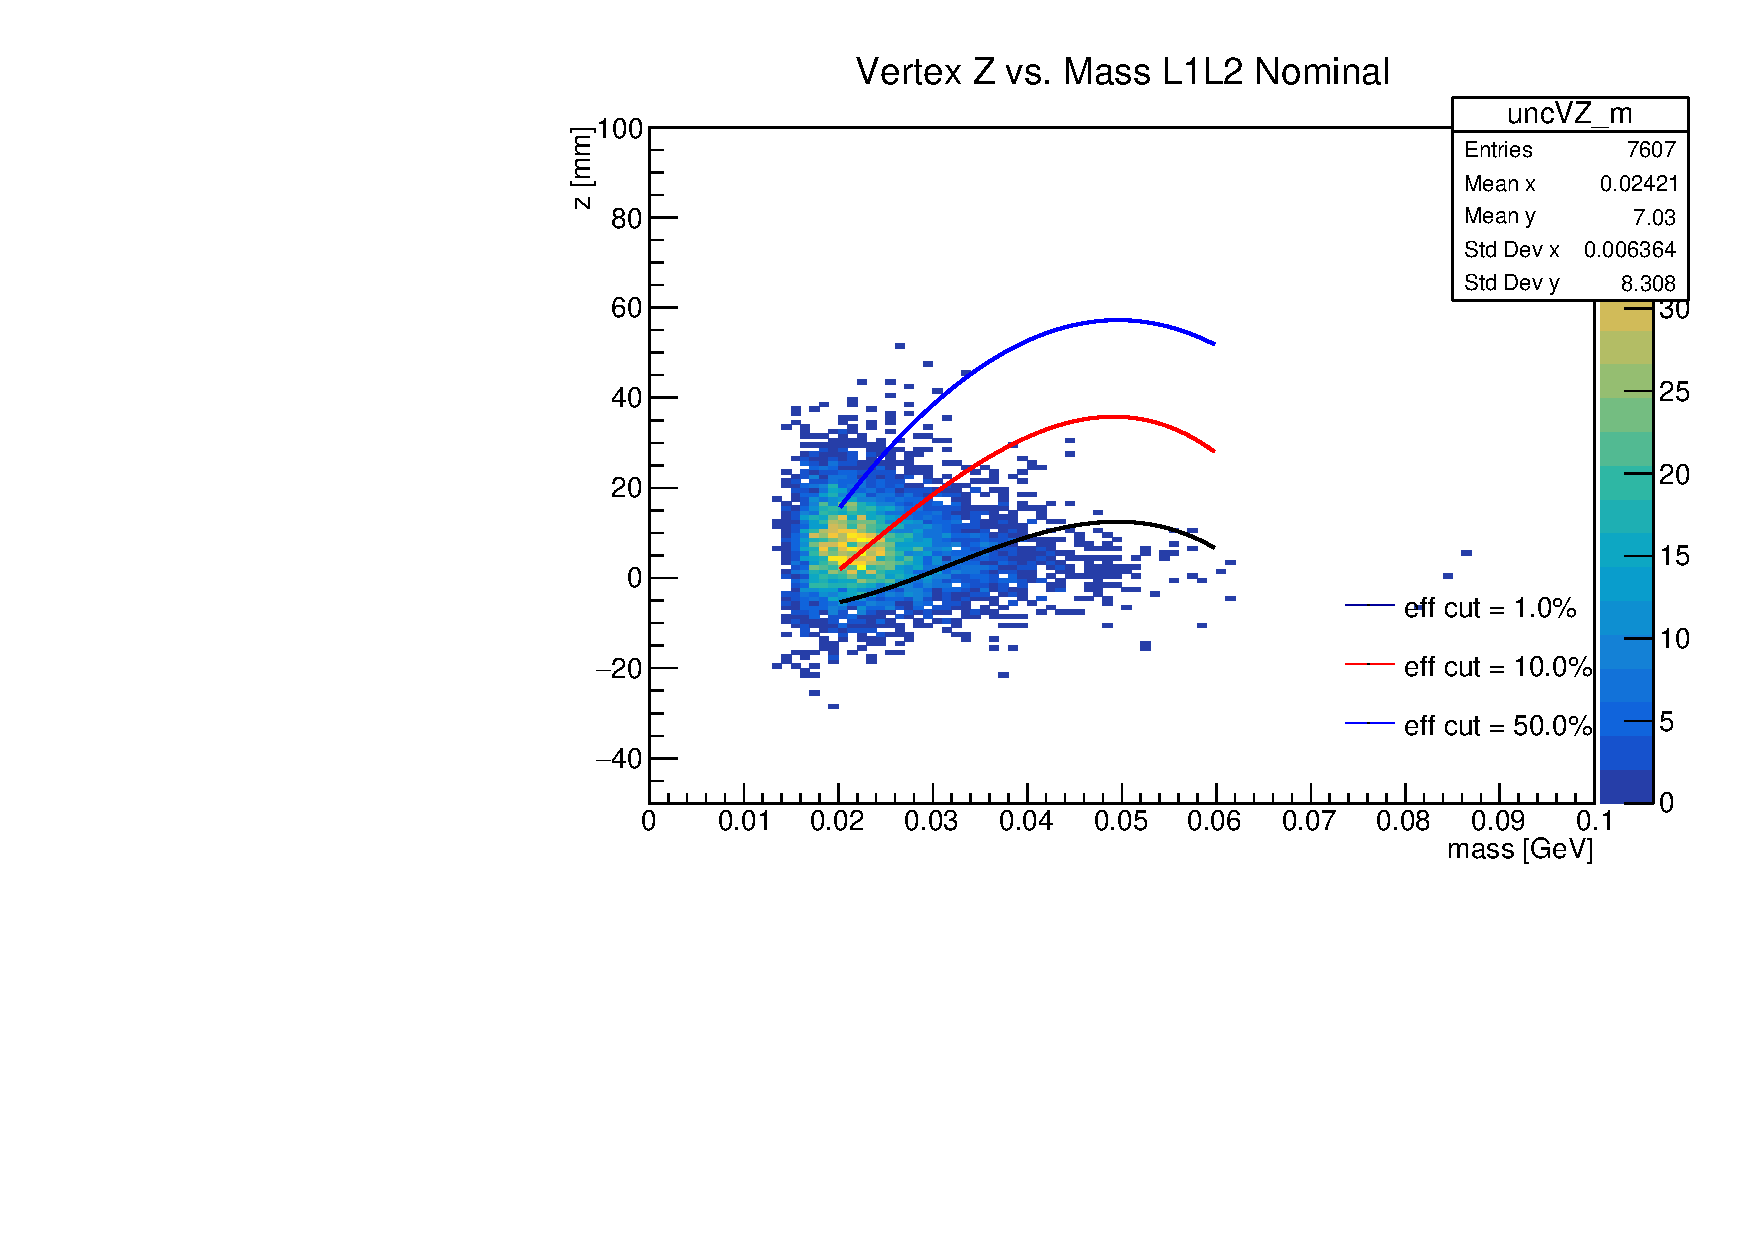
\includegraphics[width=0.4\linewidth]{figs/L1L2_sharedcut.pdf}
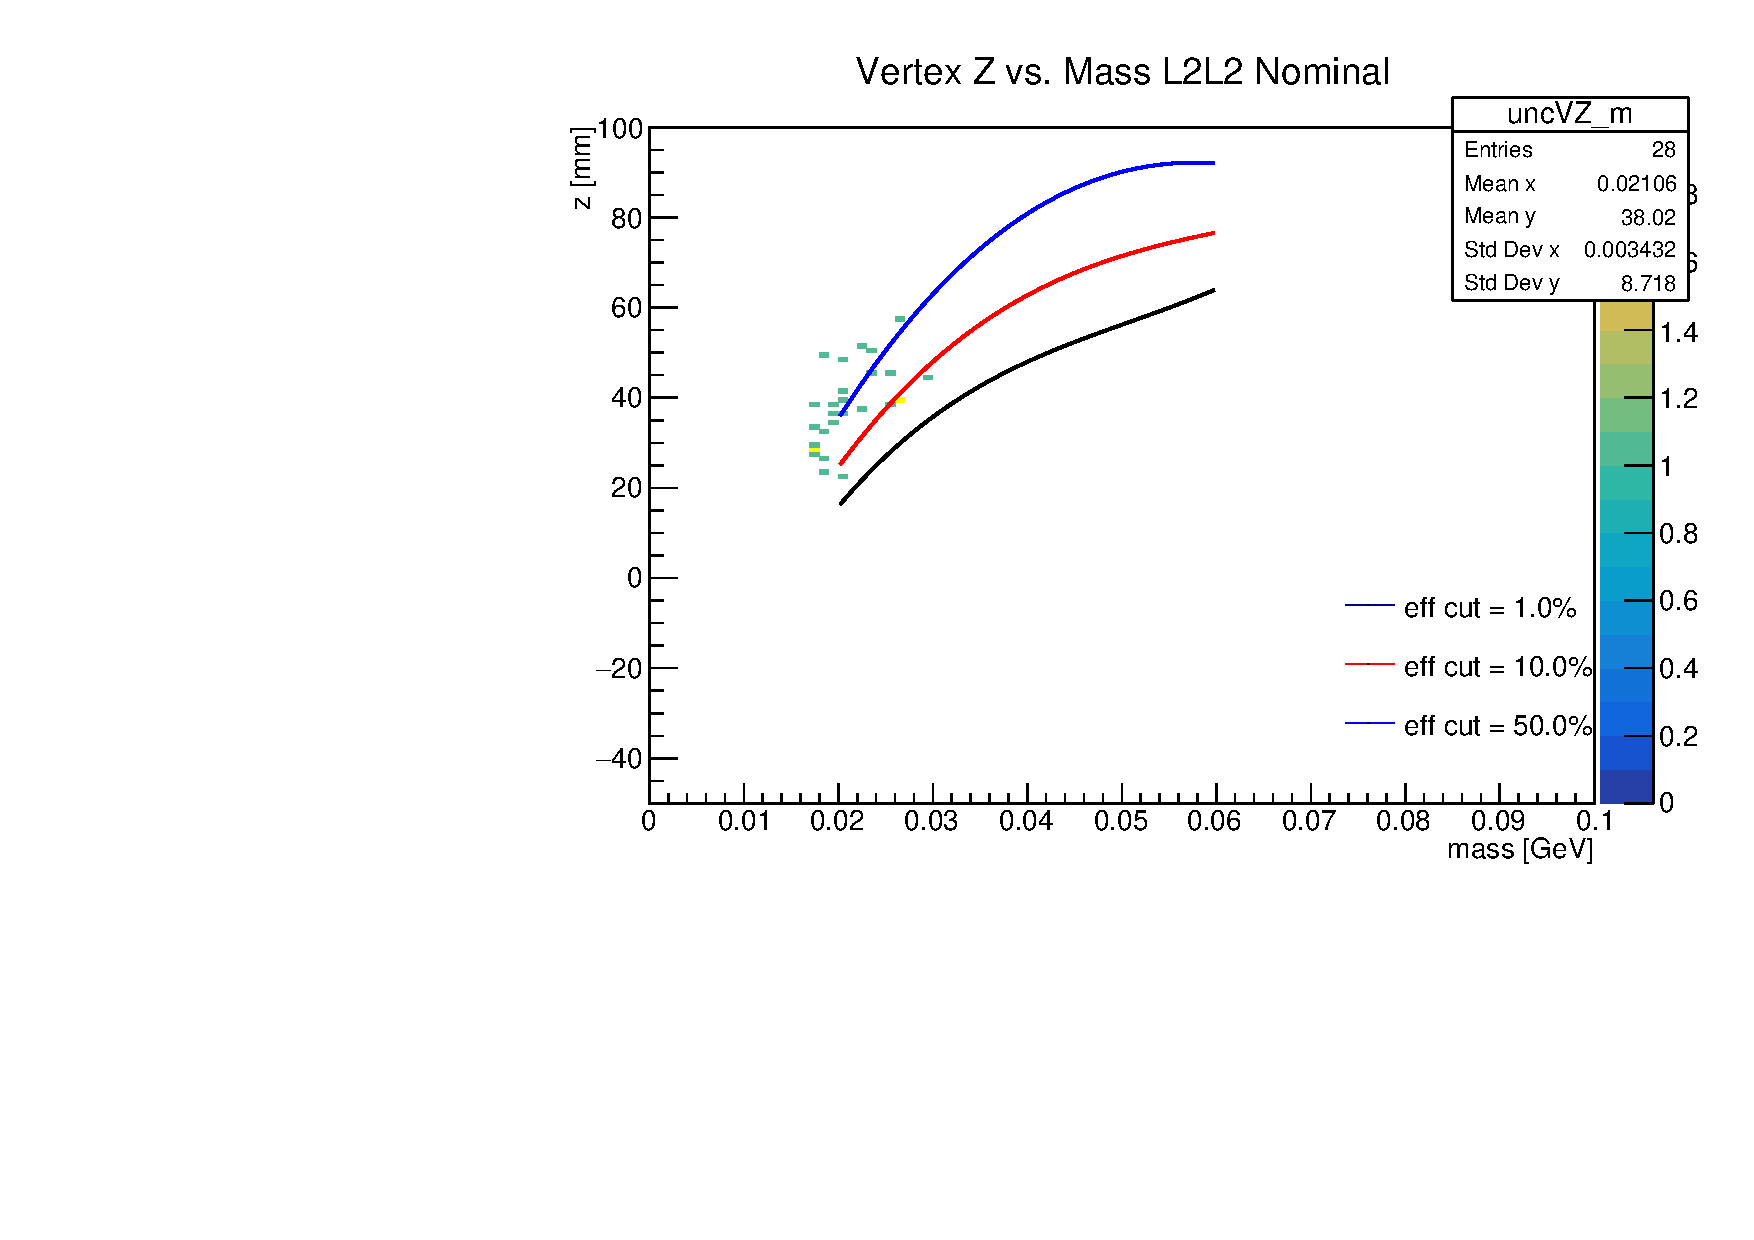
\includegraphics[width=0.4\linewidth]{figs/L2L2_sharedcut.pdf}
\end{figure}

\end{frame}

%------------------------------------------------

\begin{frame}
\frametitle{Other Layer Requirements Vz vs. Mass Upgrade Detector}
\begin{figure}
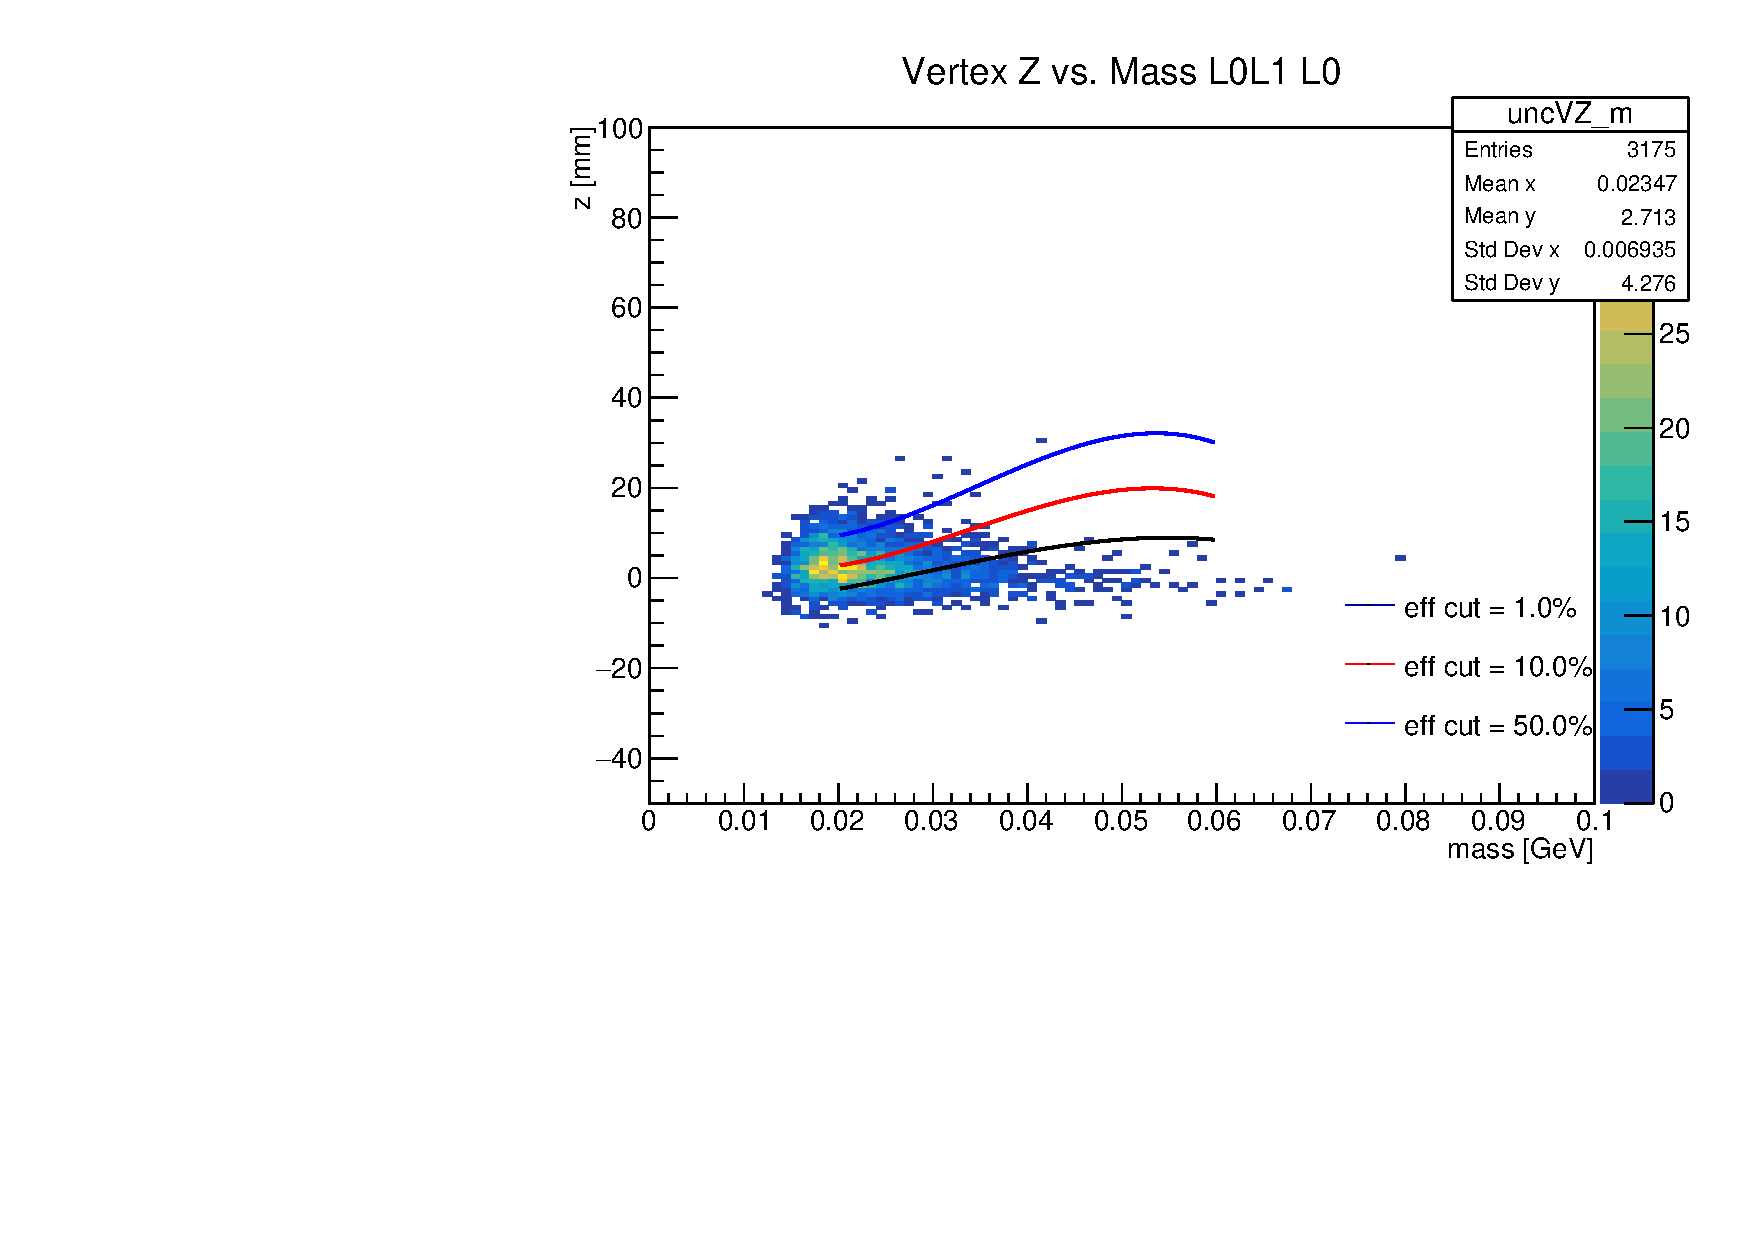
\includegraphics[width=0.4\linewidth]{figs/L0L1_loose.pdf}
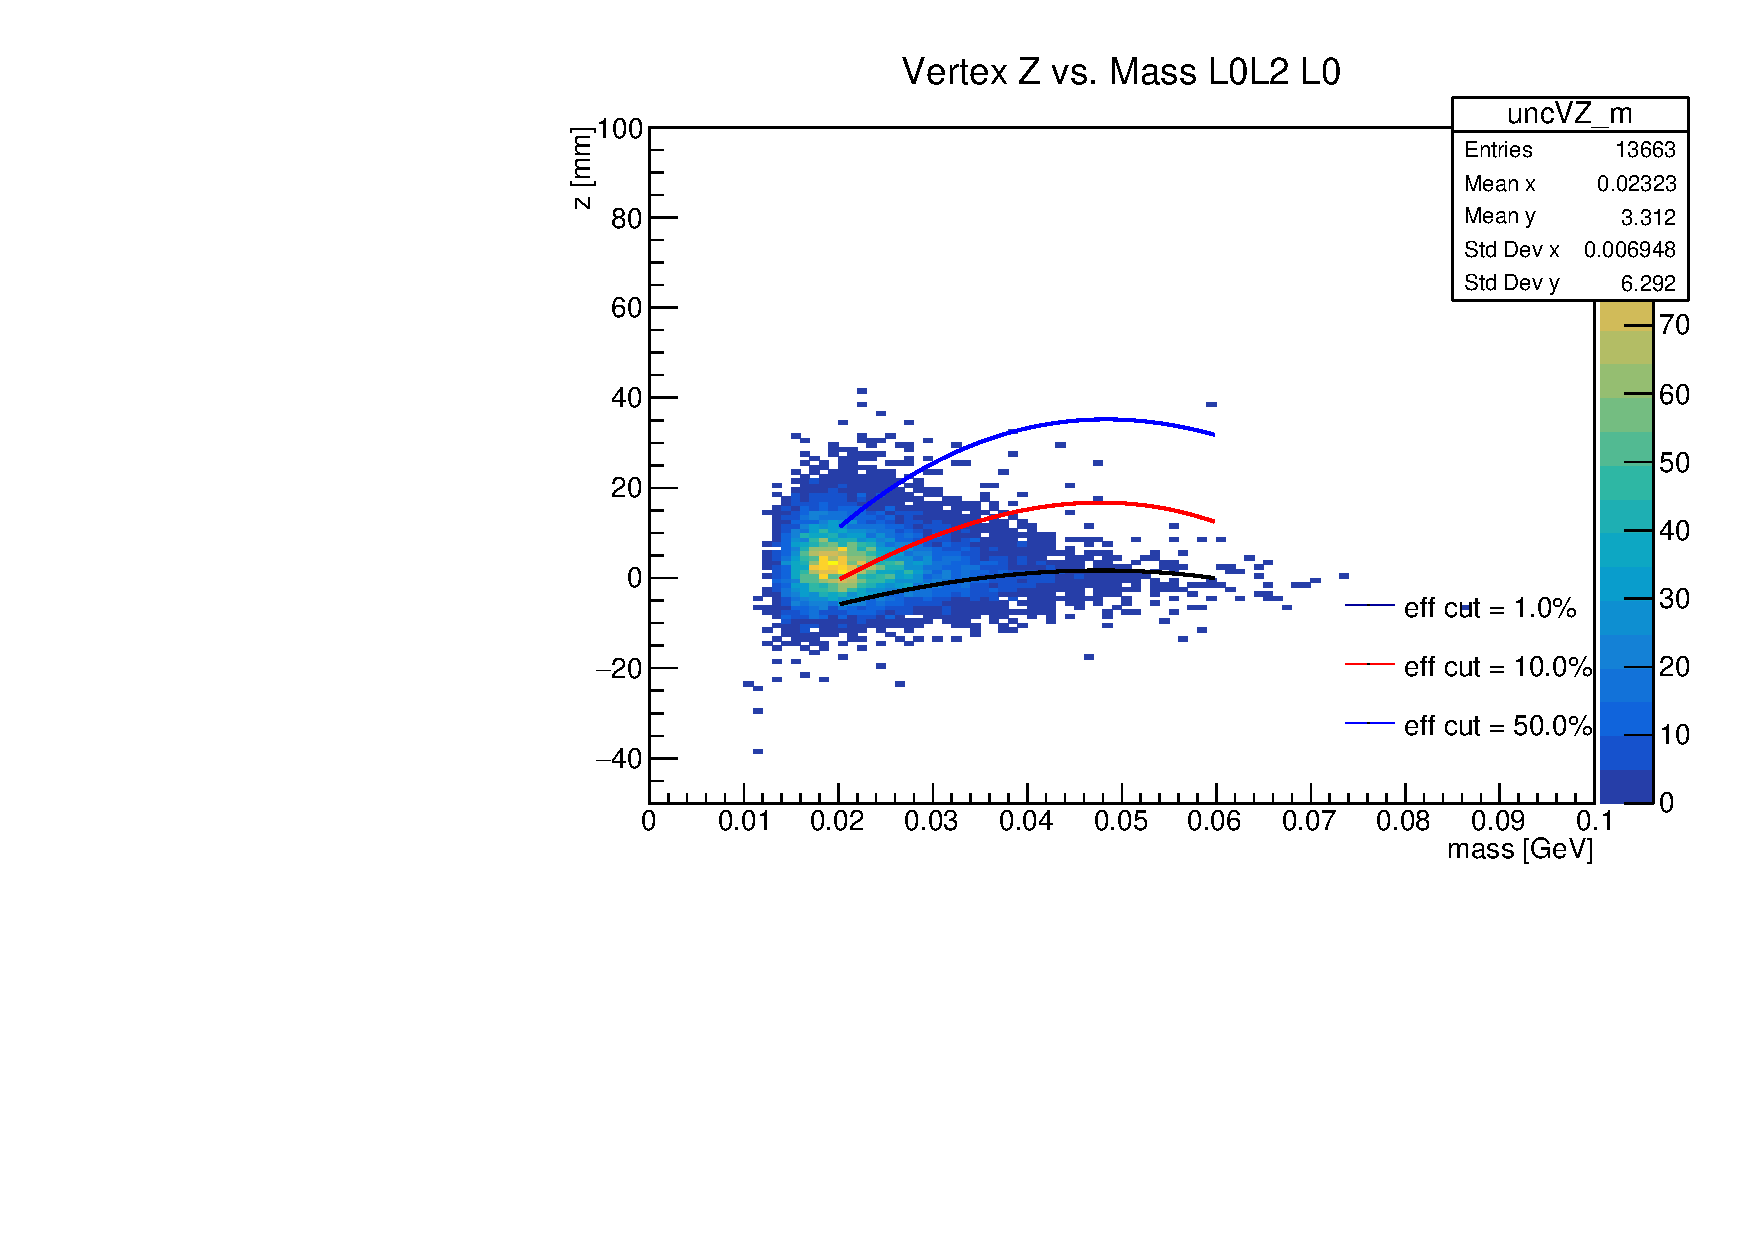
\includegraphics[width=0.4\linewidth]{figs/L0L2_loose.pdf}
\end{figure}
\begin{figure}
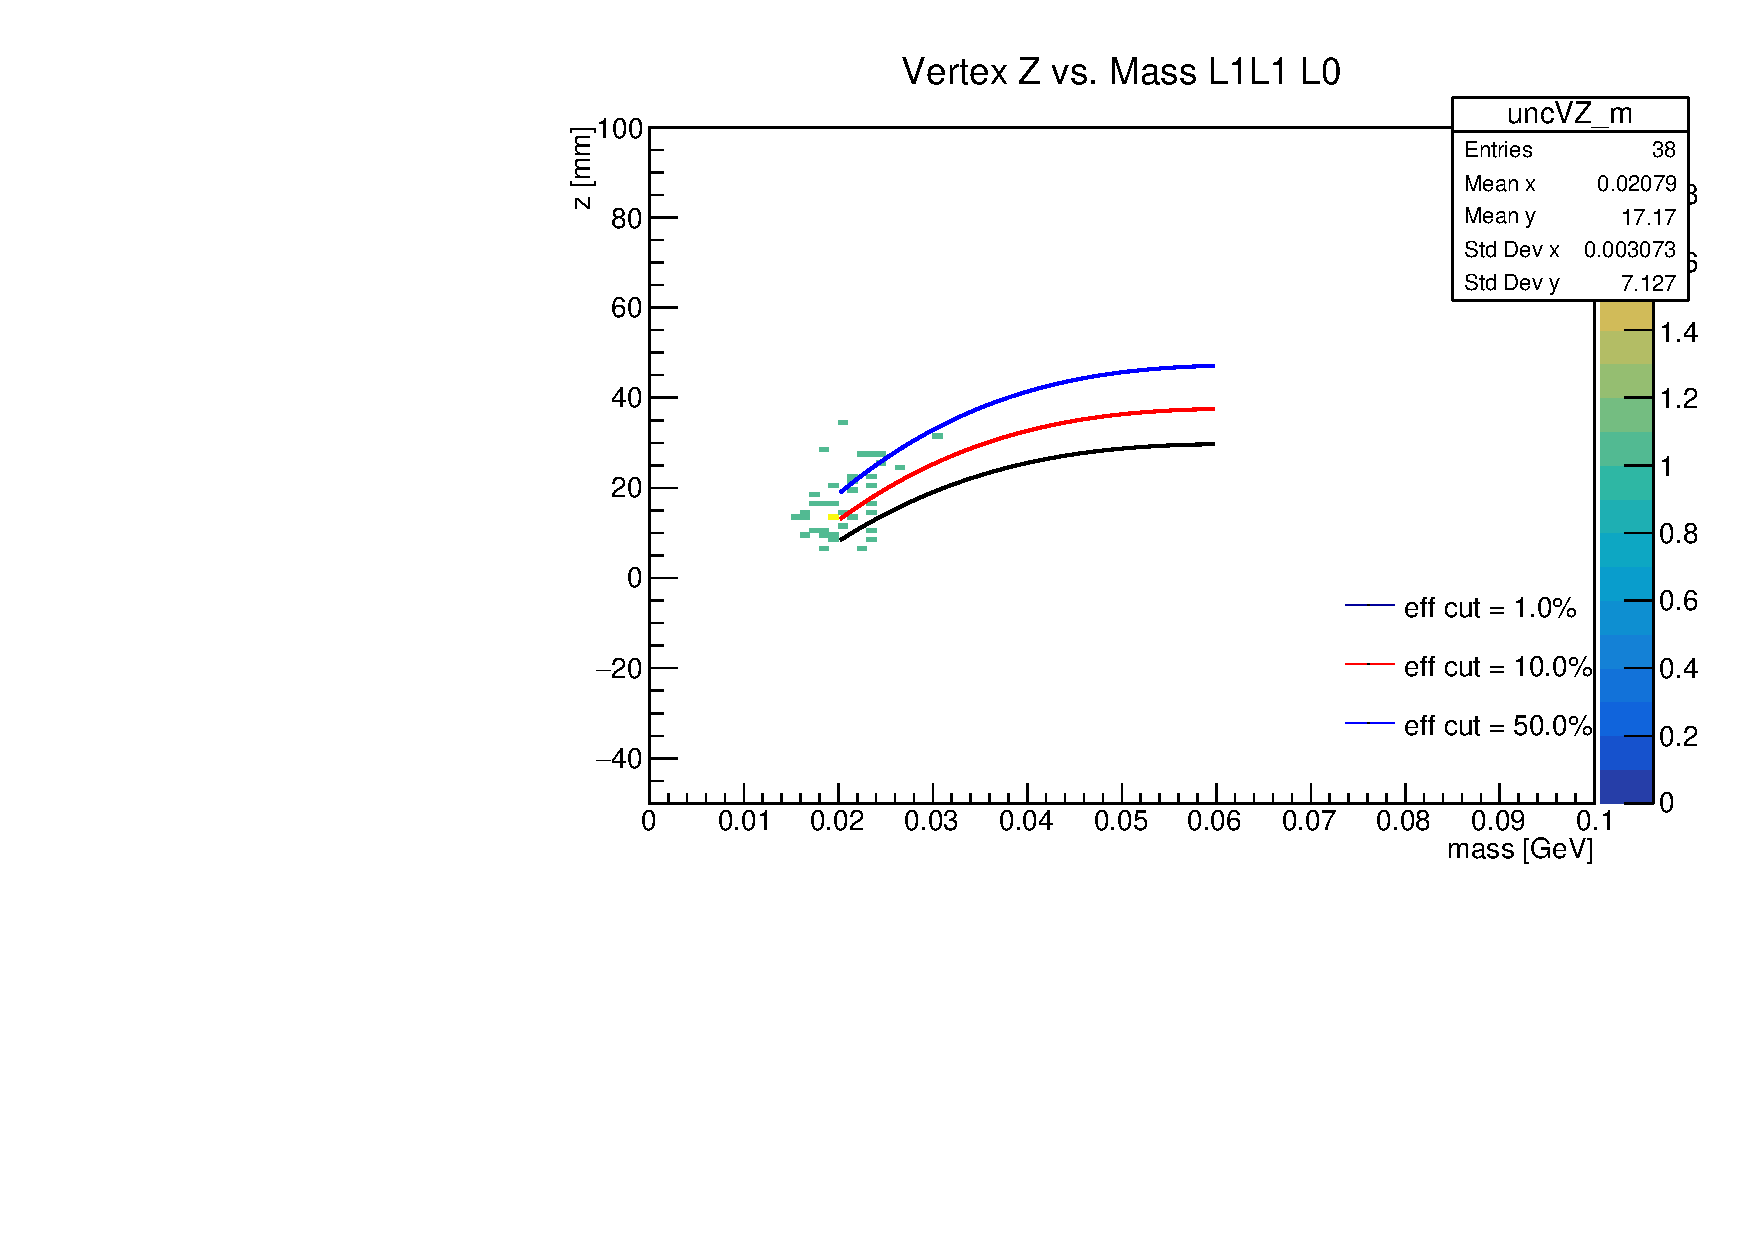
\includegraphics[width=0.4\linewidth]{figs/L1L1_loose.pdf}
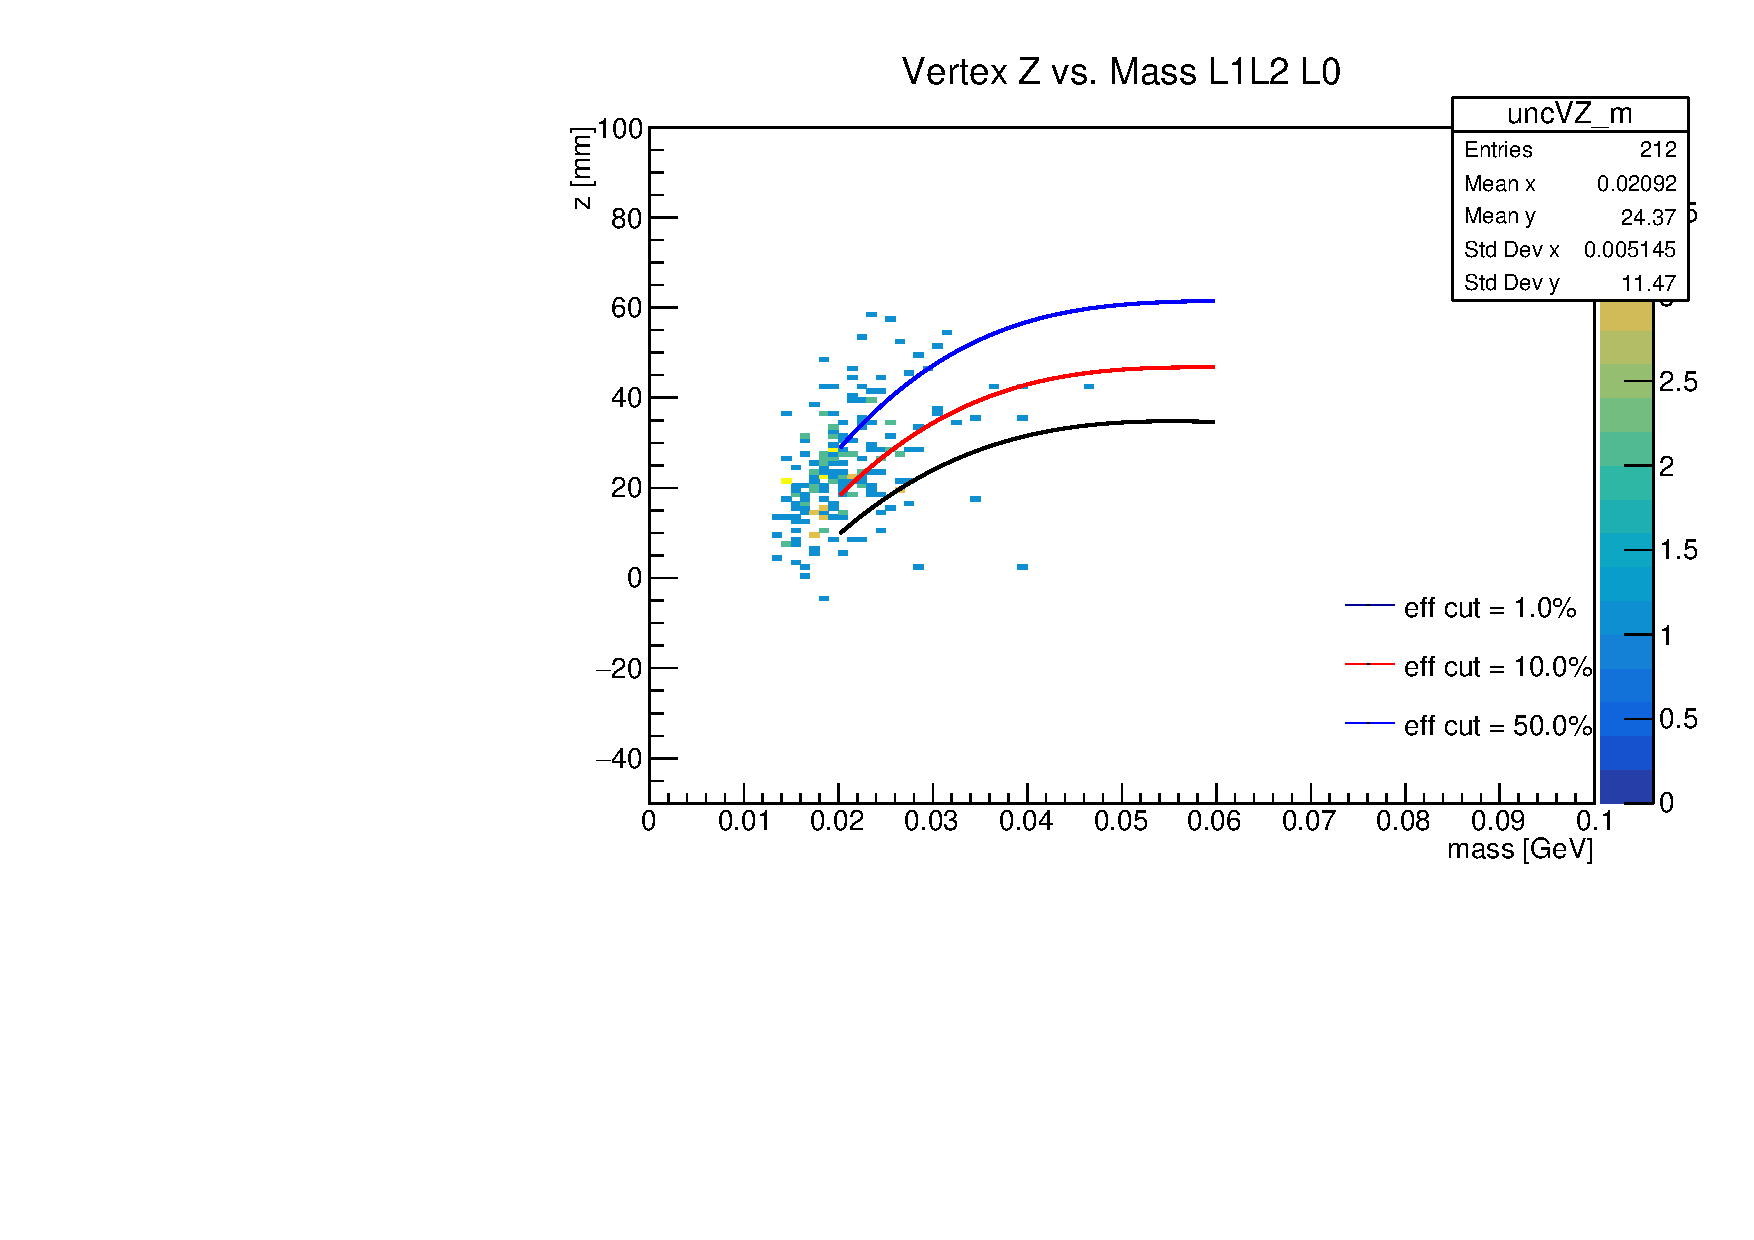
\includegraphics[width=0.4\linewidth]{figs/L1L2_loose.pdf}
\end{figure}

\end{frame}

%------------------------------------------------

\begin{frame}
\frametitle{Backgrounds}
\begin{itemize}
\item Backgrounds produced at the target remain the same in upgrade detector
\item Increased multiple scattering due to silicon (L0) in tracker which is accounted for in the previous analysis
\item \textcolor{darkgray}{\textbf{Increased converted wabs due to extra silicon}} (L0) and moving silicon into \textcolor{darkgray}{\textbf{lower angular acceptance}} (L2 and L3)
\item \textcolor{darkgray}{\textbf{Trigger rate is 30 kHz for L0 and 22 kHz for nominal}}
\end{itemize}
\begin{figure}
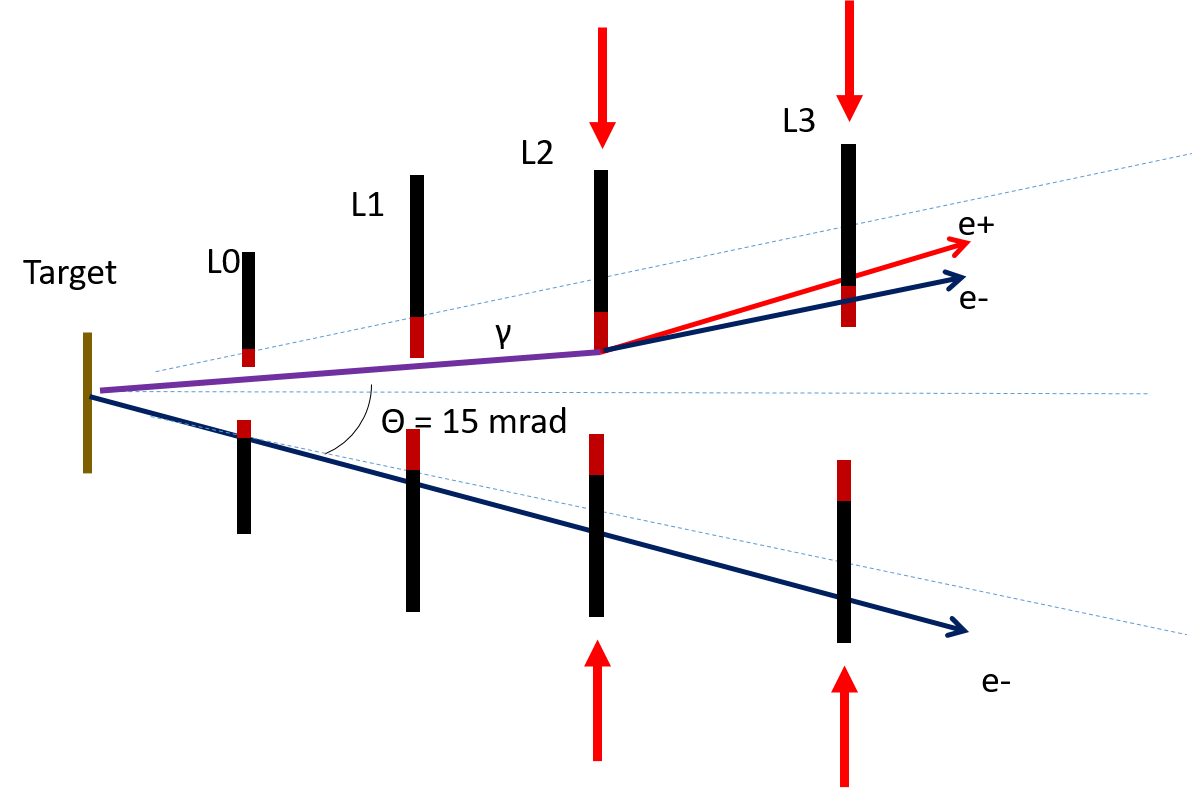
\includegraphics[width=0.5\linewidth]{figs/background_schematic.png}
\end{figure}

\end{frame}

%------------------------------------------------

\begin{frame}
\frametitle{Backgrounds - Increased Wabs due to L0}
\begin{itemize}
\item Only beamspot $\chi^2$ (for bad track fits) and isolation cuts (for mis-hits) are present
\item There is clearly a large rate increase at L0 due to converted wabs
\item The remainder of \textcolor{darkgray}{\textbf{vertexing cuts eliminates these events}}
\end{itemize}
\begin{figure}
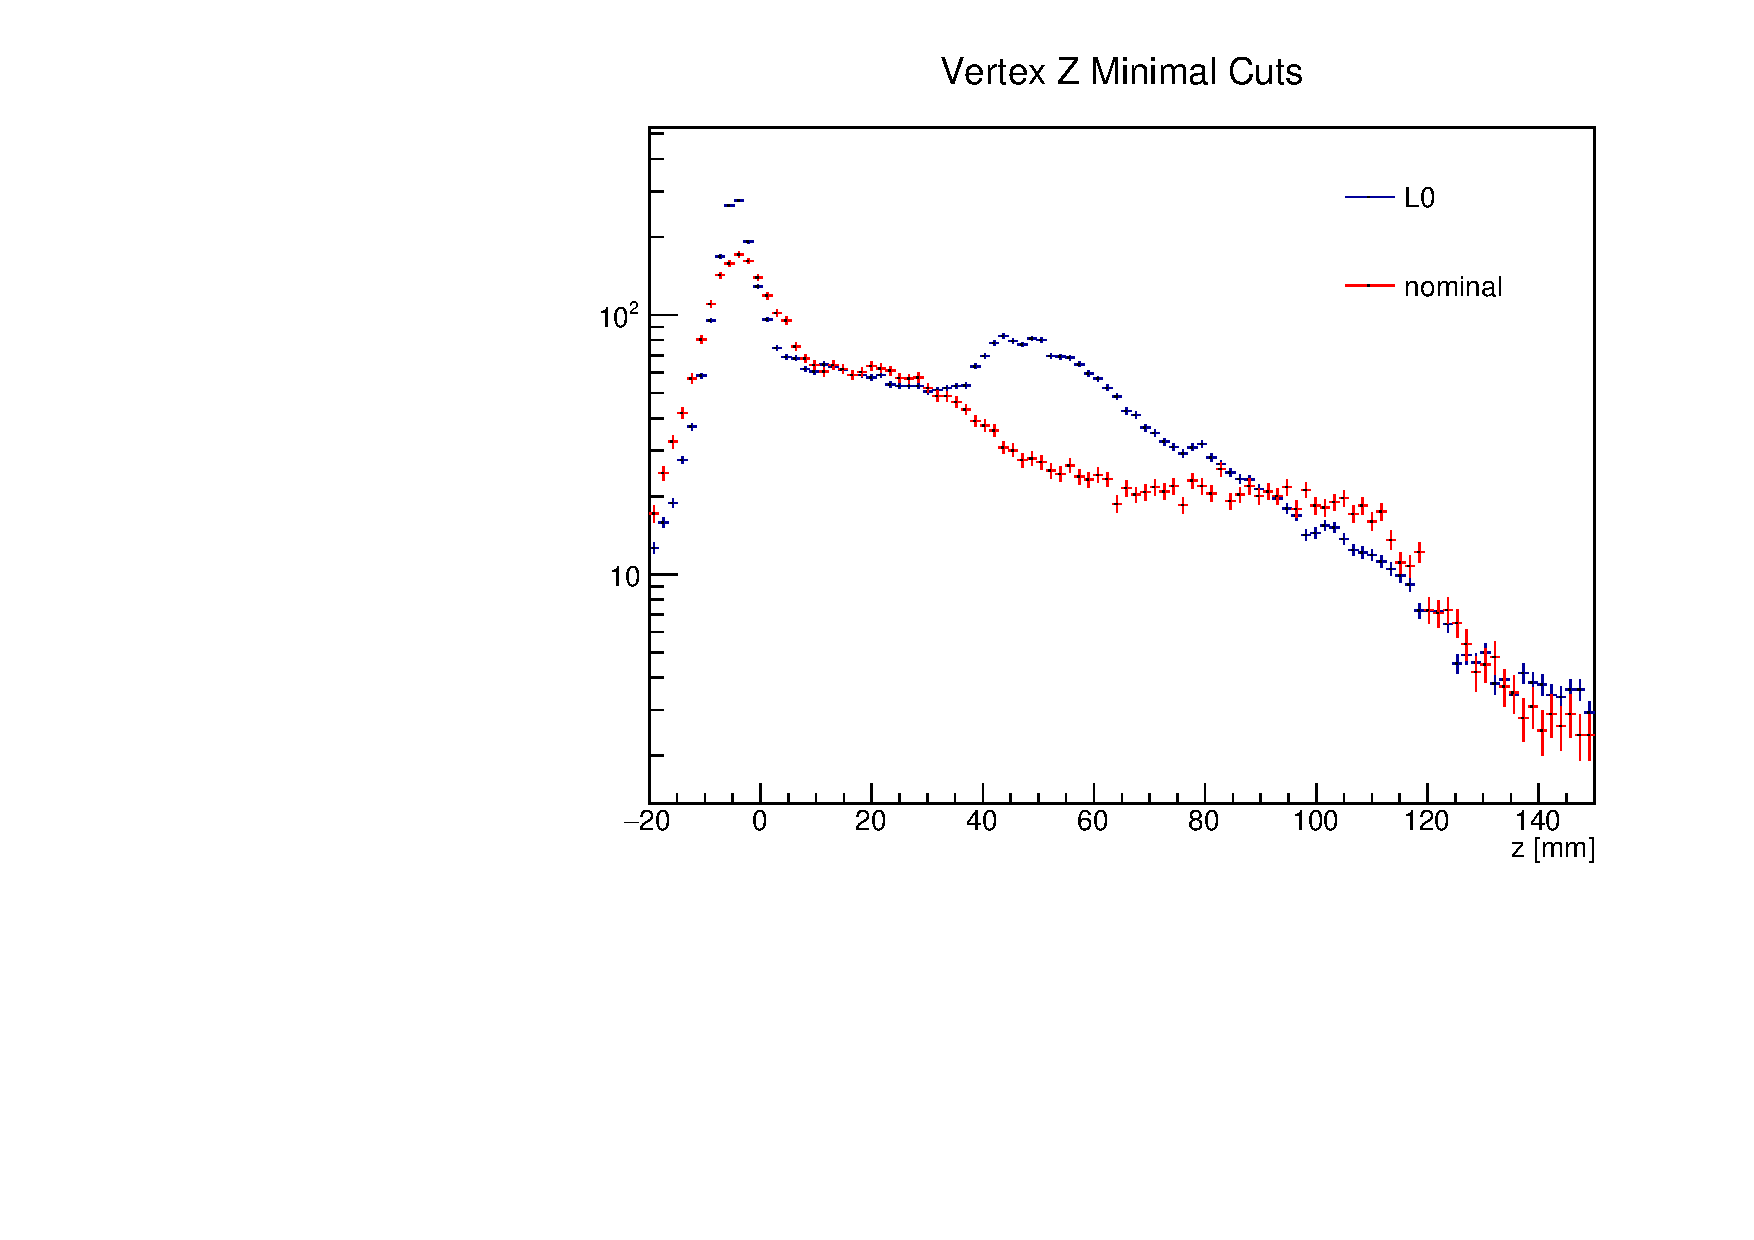
\includegraphics[width=0.4\linewidth]{figs/log_uncVZ.pdf}
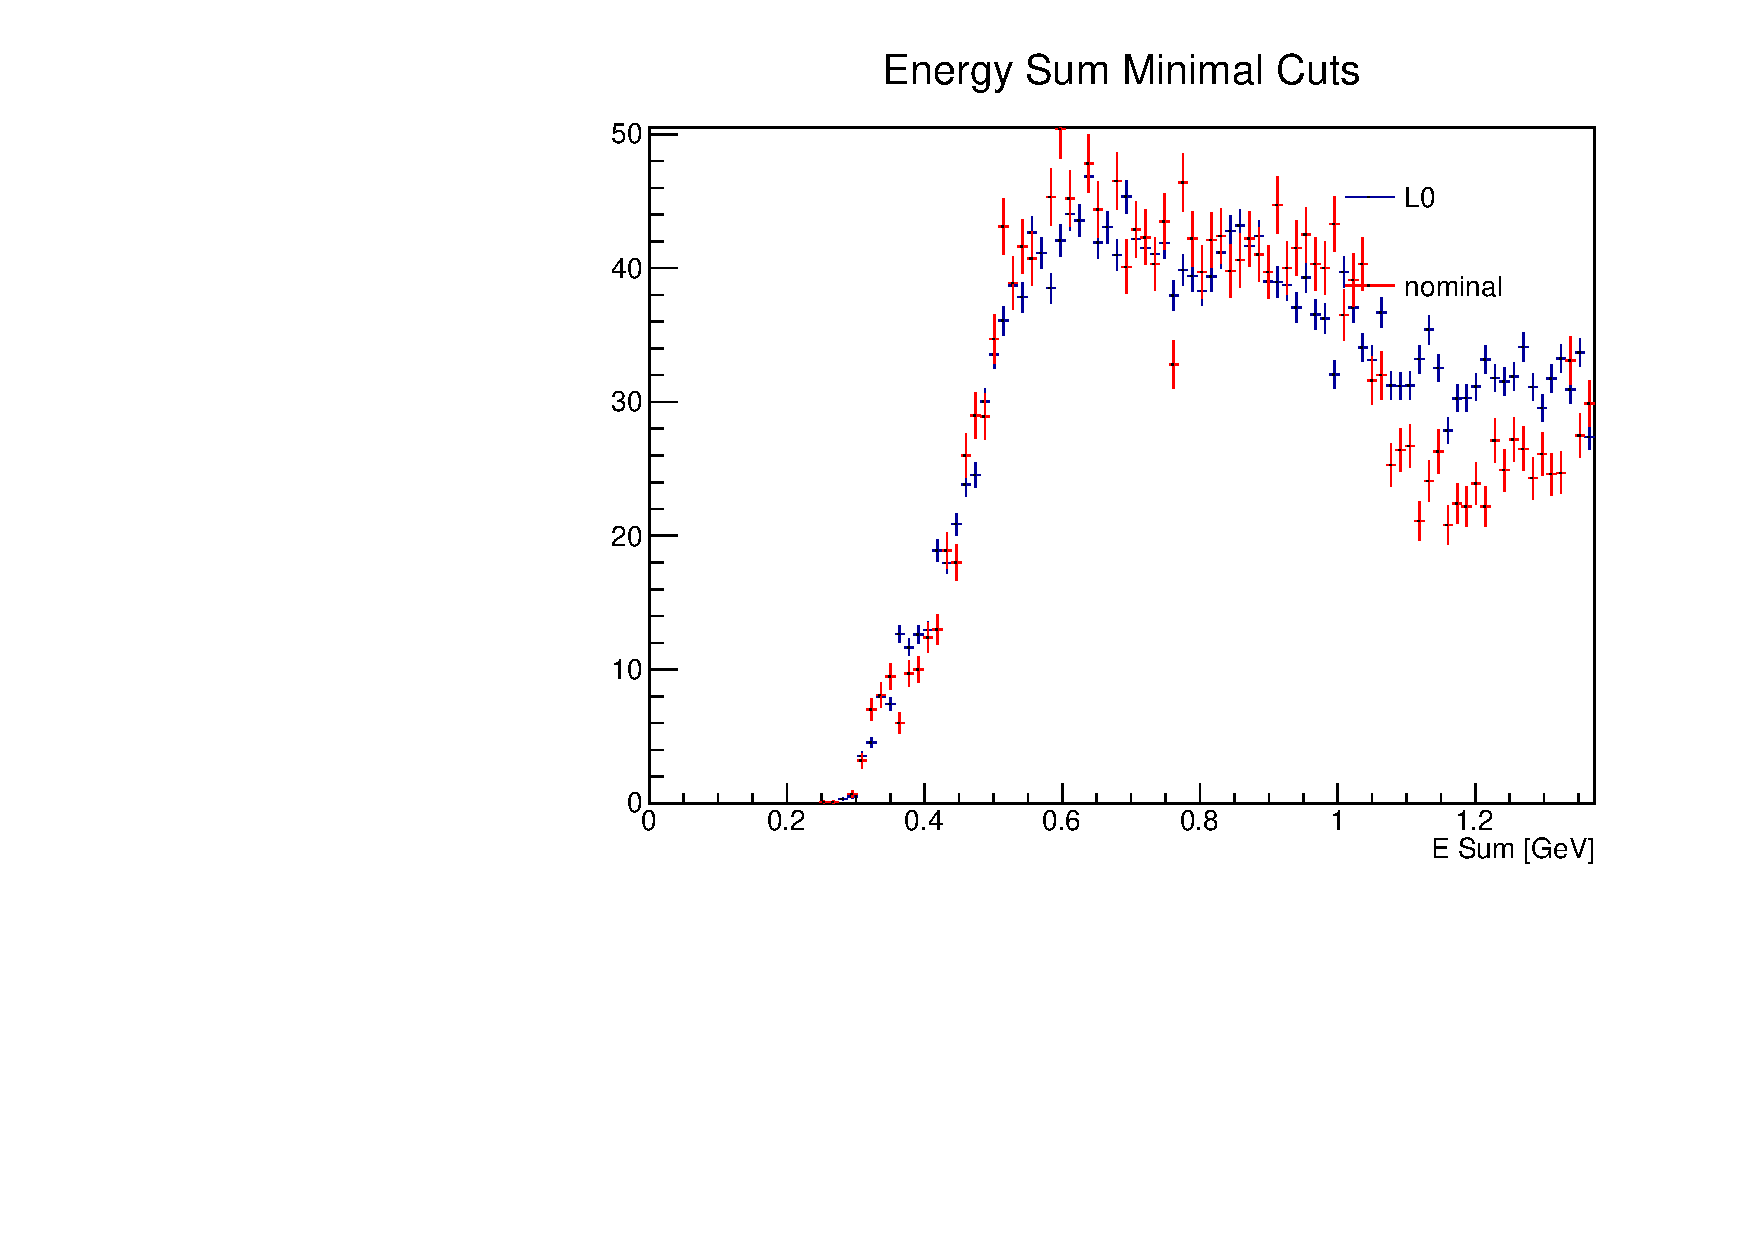
\includegraphics[width=0.4\linewidth]{figs/Esum.pdf}
\end{figure}

\end{frame}

%------------------------------------------------

\begin{frame}
\frametitle{Backgrounds - Increased Wabs due to L2 and L3}
\begin{itemize}
\item Large rate increase for electrons below 15 mrad (due to L2 and L3 moving towards the beam)
\item Requiring opposite volumes of electrons/positrons \textcolor{darkgray}{\textbf{minimizes this rate increase}}
\end{itemize}
\begin{figure}
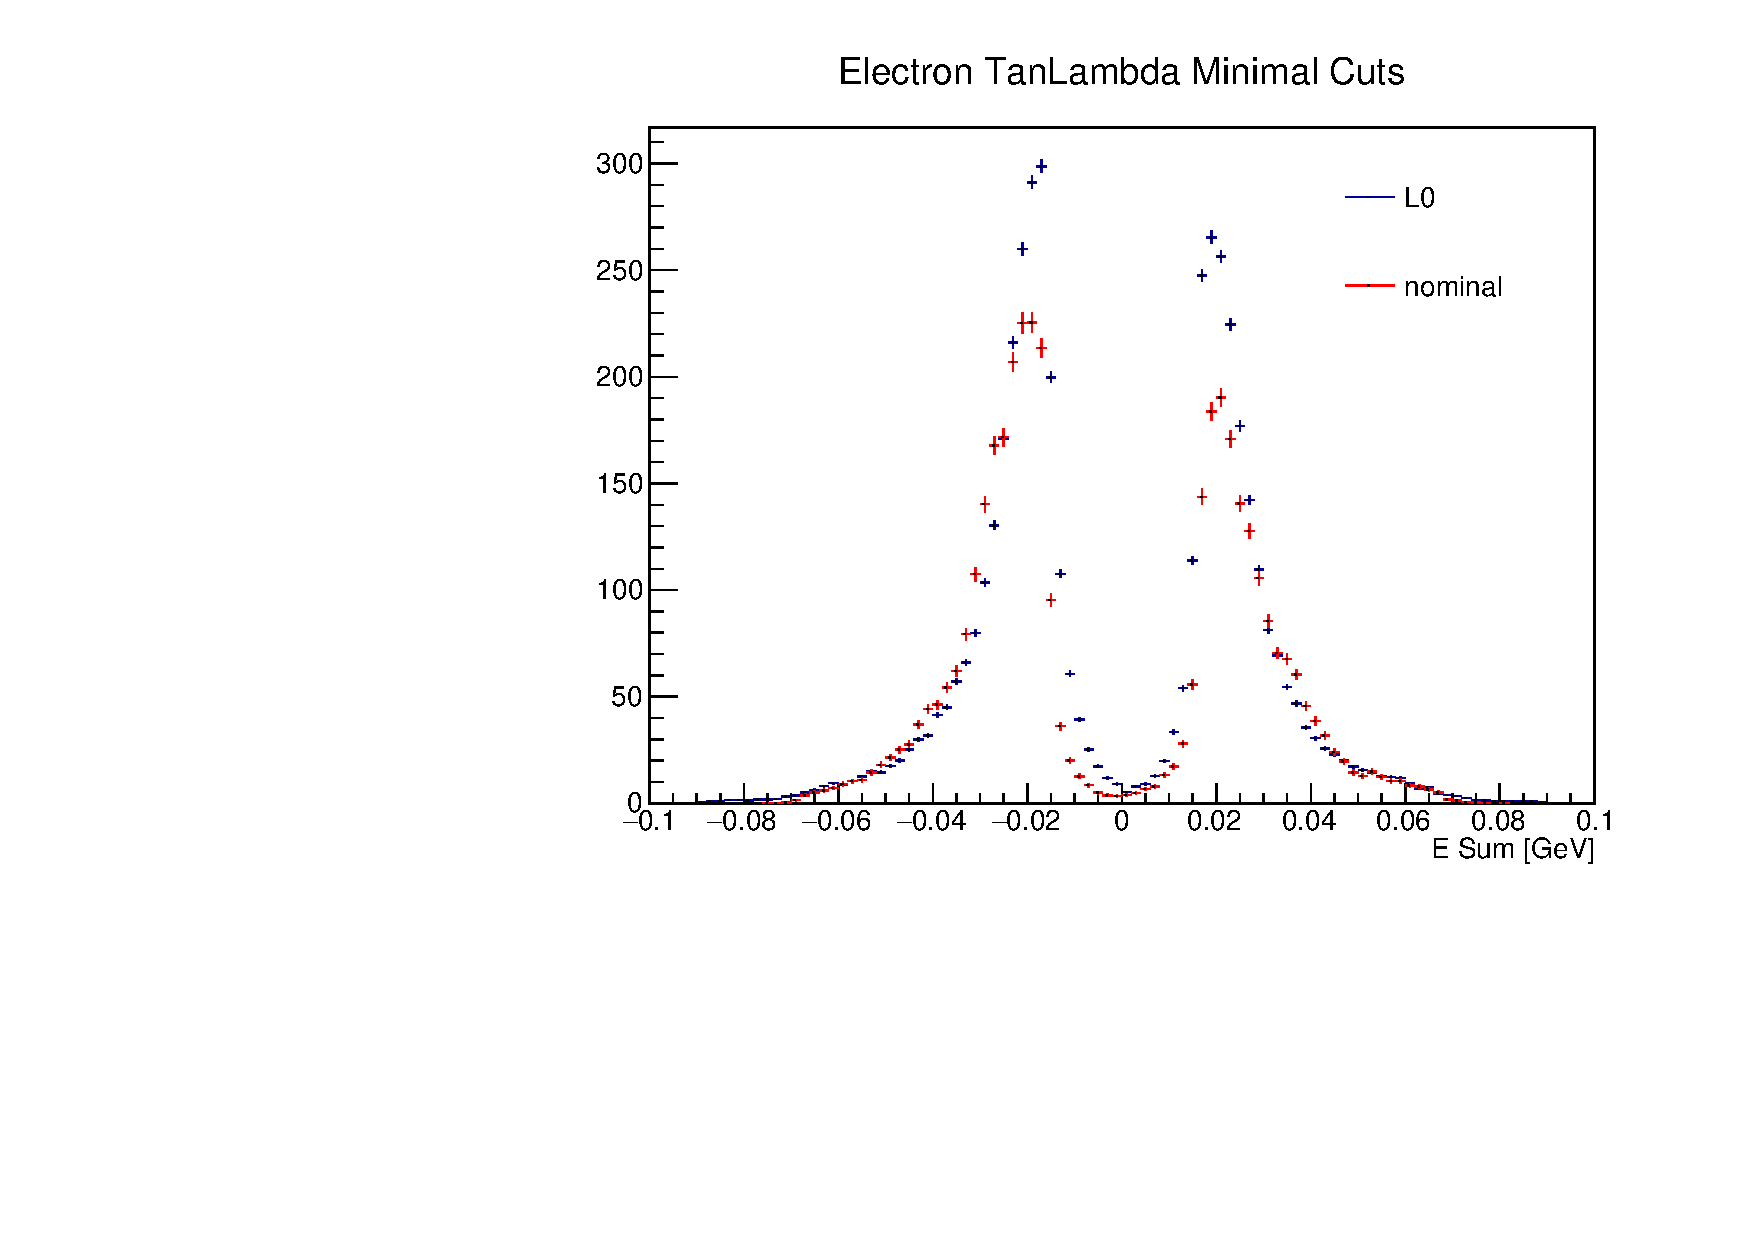
\includegraphics[width=0.5\linewidth]{figs/eleLambda.pdf}
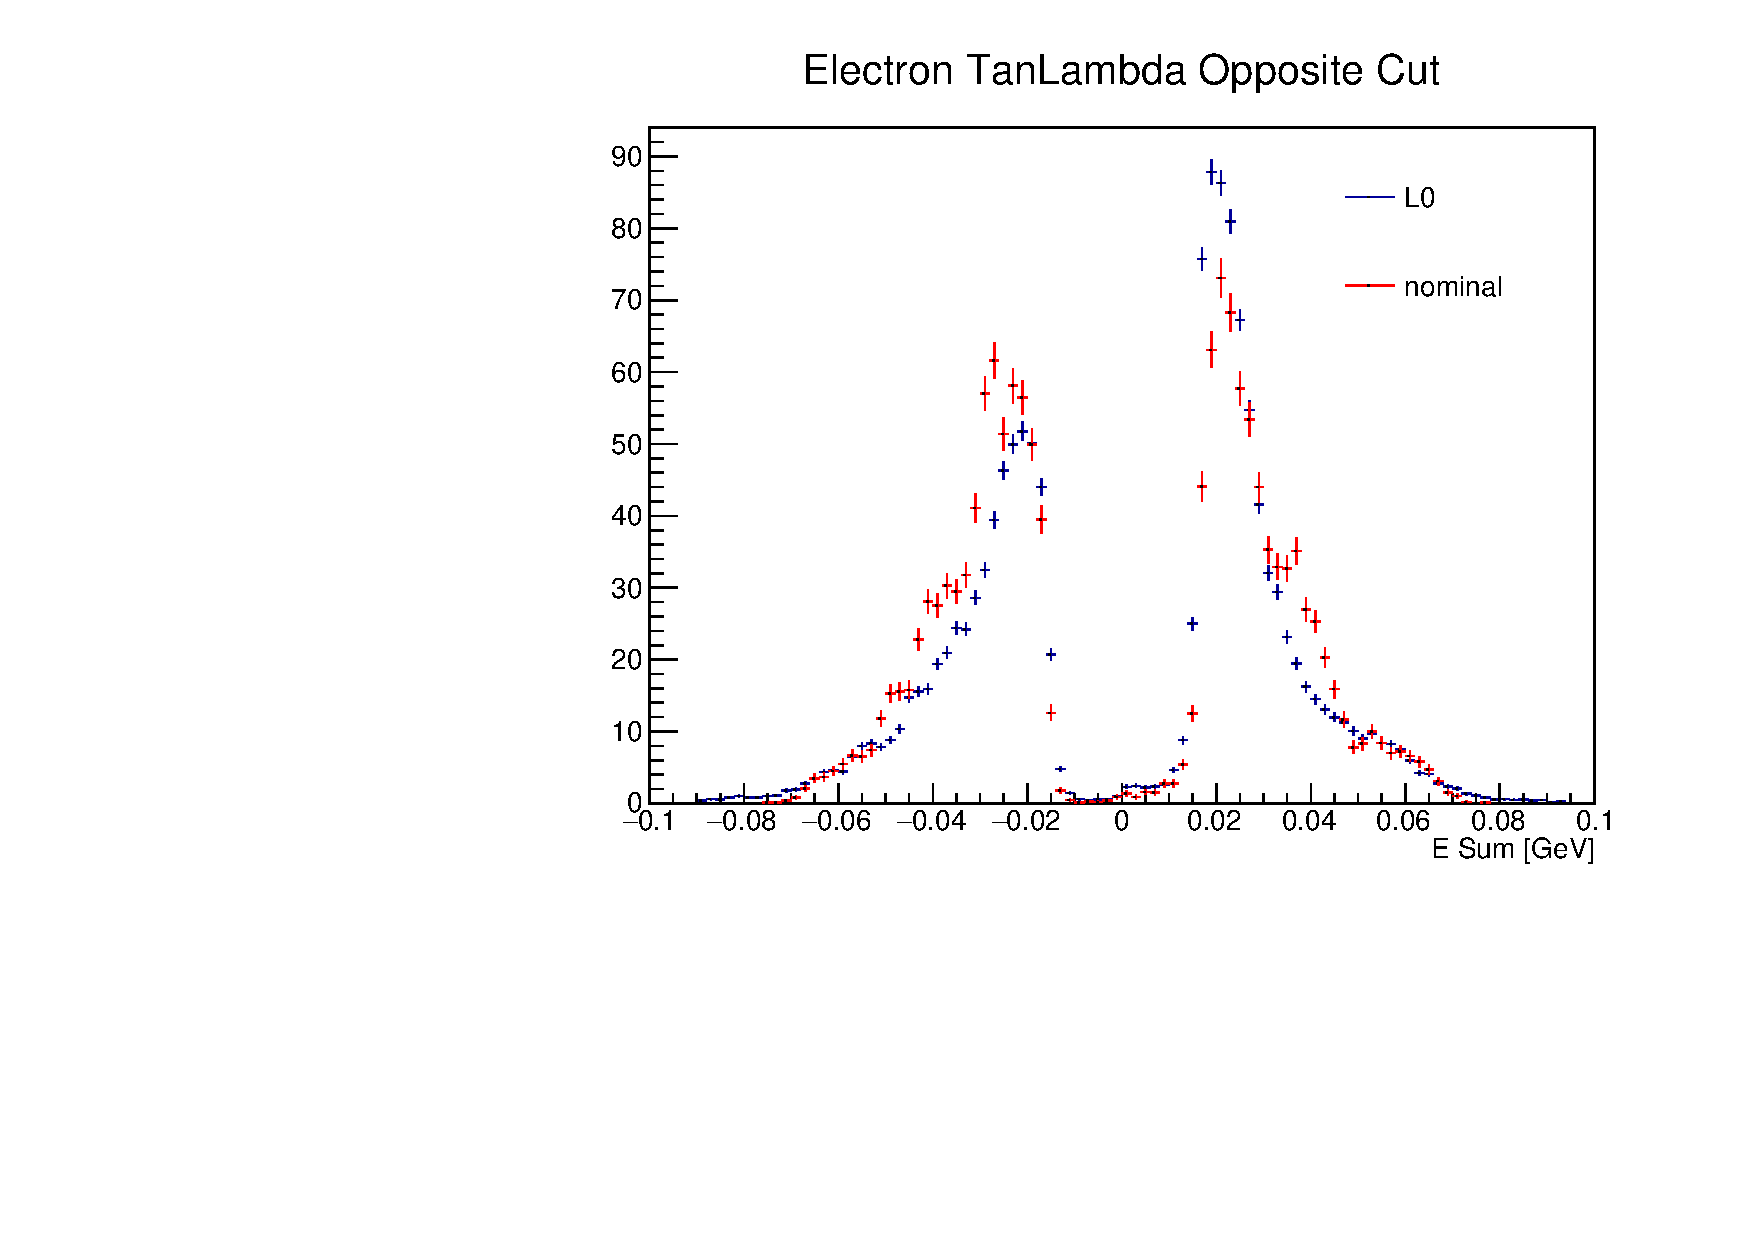
\includegraphics[width=0.5\linewidth]{figs/eleLambda_oppo.pdf}
\end{figure}

\end{frame}

%------------------------------------------------

%\begin{frame}
%\frametitle{Backgrounds - Occupancies}
%\begin{itemize}
%\item Occupancies for Layer 0
%\end{itemize}
%\begin{figure}
%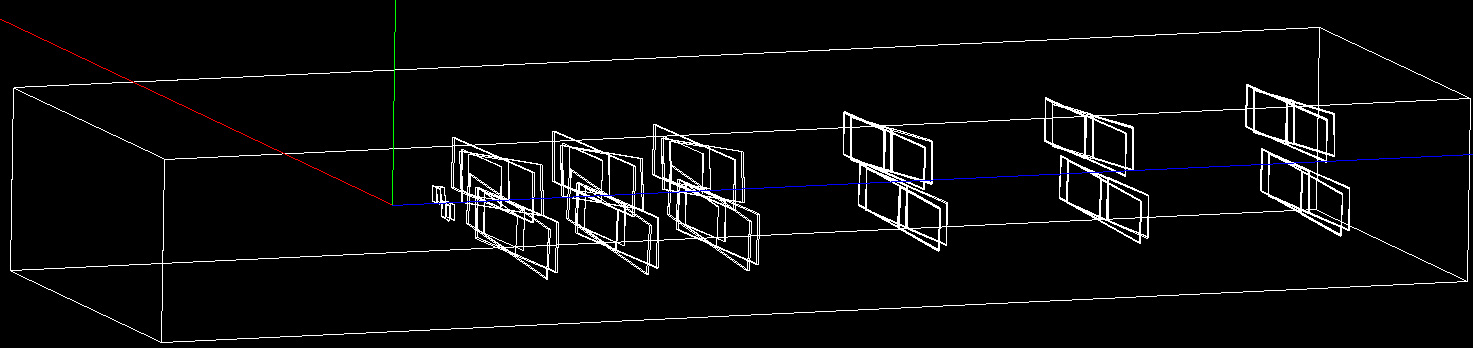
\includegraphics[width=0.4\linewidth]{figs/L0_schematic.png}
%\end{figure}

%\end{frame}

%------------------------------------------------

%\begin{frame}
%\frametitle{Backgrounds - Occupancies (cont.)}
%\begin{itemize}
%\item Comparison of occupancies for top (left) and bottom (right)
%\end{itemize}
%\begin{figure}
%\includegraphics[width=0.4\linewidth]{figs/L0_schematic.png}
%\end{figure}

%\end{frame}

%------------------------------------------------

\begin{frame}
\frametitle{Future Work}
\begin{itemize}
\item \textcolor{darkgray}{\textbf{Mix correct fraction of wabs into the MC}} and solve other MC issues
\item More carefully optimize cuts for L0, currently cutting out too many events (also solve other minor problems)
\item Obtain total reach from all exclusive layer requirements (very challenging)
\begin{itemize}
\item Vertex pulls and impact parameter cuts seem promising
\end{itemize}
\item Recoil electron acceptance studies and occupancy studies
\item \textcolor{darkgray}{\textbf{Do it all again for 2.3 GeV!}}
\item Open for ideas (but not too open...)
\end{itemize}

\end{frame}

%------------------------------------------------

\begin{frame}
\frametitle{Conclusion}
\begin{itemize}
\item Adding a tracking layer between the target and current first layer \textcolor{darkgray}{\textbf{improves vertex resolution by about a factor of 2}} in all relevant beam energies, and hence improves the zcut
\item By simply requiring first layer hits, the \textcolor{darkgray}{\textbf{L0 detector shows a drastic improvement in reach}} compared to the current setup for 1.05 GeV
\item It is reasonable to say that \textcolor{darkgray}{\textbf{reach will improve significantly for other relevant beam energies}}
\item Moving in tracking layers 2 and 3 in by 0.8 mm \textcolor{darkgray}{\textbf{improves displaced A' detection acceptance}}
\item Mass resolution also improves slightly, and \textcolor{darkgray}{\textbf{background rates are manageable}}
\item It is recommended that \textcolor{darkgray}{\textbf{L0 production proceed ASAP}} (Tim)
\end{itemize}
%\begin{figure}
%\includegraphics[width=0.4\linewidth]{figs/L0_180_days.pdf}
%\end{figure}

\end{frame}

%------------------------------------------------

\begin{frame}
\frametitle{Backup Slides}

\begin{itemize}
\item MC Rate Comparisons
\end{itemize}

\begin{figure}
\includegraphics[width=0.55\linewidth]{figs/psum.pdf}
\includegraphics[width=0.55\linewidth]{figs/psum_L0.pdf}
\end{figure}

\end{frame}

%------------------------------------------------

\begin{frame}
\frametitle{Backup Slides}

\begin{itemize}
\item Vertex Z for background simulation using vertexing cuts
\end{itemize}

\begin{figure}
\includegraphics[width=0.55\linewidth]{figs/log_uncVZ_vertcuts.pdf}
\end{figure}

\end{frame}

%------------------------------------------------

\begin{frame}
\frametitle{Backup Slides}

\begin{itemize}
\item Number of A's detectable for 4 weeks for L0 (left) and nominal (right)
\end{itemize}

\begin{figure}
\includegraphics[width=0.5\linewidth]{figs/detectable_4_weeks_L0.png}
\includegraphics[width=0.5\linewidth]{figs/detectable_4_weeks_nom.png}
\end{figure}

\end{frame}

%------------------------------------------------

\begin{frame}
\frametitle{Backup Slides}

\begin{itemize}
\item Number of A's detectable for 10 weeks for L0 (left) and nominal (right)
\end{itemize}

\begin{figure}
\includegraphics[width=0.5\linewidth]{figs/detectable_10_weeks_L0.png}
\includegraphics[width=0.5\linewidth]{figs/detectable_10_weeks_nom.png}
\end{figure}

\end{frame}

%------------------------------------------------

\begin{frame}
\frametitle{Backup Slides}

\begin{itemize}
\item Number of A's detectable for 180 days for L0 (left) and nominal (right)
\end{itemize}

\begin{figure}
\includegraphics[width=0.5\linewidth]{figs/detectable_180_days_L0.png}
\includegraphics[width=0.5\linewidth]{figs/detectable_180_days_nom.png}
\end{figure}

\end{frame}

%------------------------------------------------

\end{document} 
